\section{Uncertainties and Systematics}
\label{sec:systematics}

Our selections are subject to some level of uncertainty, both statistical and systematic. 
The systematic uncertainties are associated to the level of precision of the model used in the simulation of the neutrino interactions (GENIE), knowledge of the neutrino beam (flux), and mis-modeling of the detector response (detector systematics). 
These systematic uncertainties can be calculated for many parameters of the models and measured variables that we use to reconstruct our sample

When treating systematic uncertainties, one wishes to take into account correlations between different bins of the distribution of a given reconstructed variable. For each uncertainty, a covariance matrix correlating the variation in the measured number of events between two bins is calculated. Two approaches are followed to obtain the covariance matrix, depending on the type of uncertainty: unisim or multisim.

Unisim means that a single variation of a given analysis input parameter is performed according to its uncertainty. The difference in the number of selected events between this variation and the central value is taken as the uncertainty in that number of events.

In the multisim procedure, several variations of a given analysis input parameter are performed. These are called universes. These different variations are obtained from a different sampling of the input parameter, which is varied within its uncertainty.
This approach allows to preserve correlations in the various bins of the distributions of selected events. 
The covariance matrix can then be obtained as

\begin{equation}
    E_{ij}^{sys} = \frac{1}{N}\sum_{k}^N (N_i^{CV} - N_i^k)(N_j^{CV} - N_j^k) ,
    \label{eqn:covmatrix}
\end{equation}

where $N$ is the total number of universes, $N_i^k$ is the value in the
$i$-th bin of the $k$-th universe and $N_i^{CV}$ is that of the central value. We utilized the SBNfit framework~\cite{bib:sbnfitgit} to construct the covariance matrices and the associated correlation matrices for our selection.

A summary of the sources of systematic uncertainty and their impact on this analysis is shown in figure~\ref{fig:systsummary}. This figure shows for the \npsel, \zpsel, and $\nu_{\mu}$ constraint selection the level of systematic uncertainty as a function of reconstructed energy. The plots further show the total constrained systematic uncertainty, obtained through the constraint procedure described in sec.~\ref{sec:sensitivity}. It is worth keeping in mind that the electron channel measurements are statistics-dominated in almost all bins, while in the \numu channel statistical errors are negligible.

\begin{figure}[H] 
\begin{center}
    \begin{subfigure}[b]{0.32\textwidth}
    \centering
    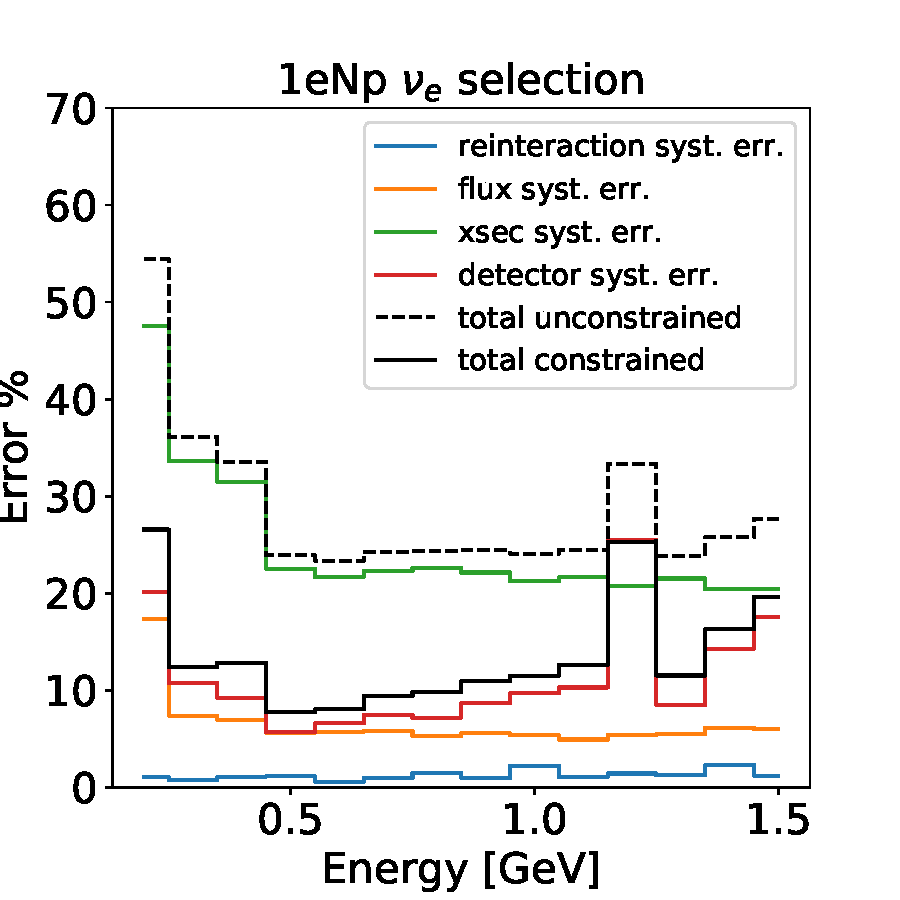
\includegraphics[width=1.00\textwidth]{Systematics/1eNp_syst_summary.pdf}
    \caption{\label{fig:systsummary:np}\npsel}
    \end{subfigure}
    \begin{subfigure}[b]{0.32\textwidth}
    \centering
    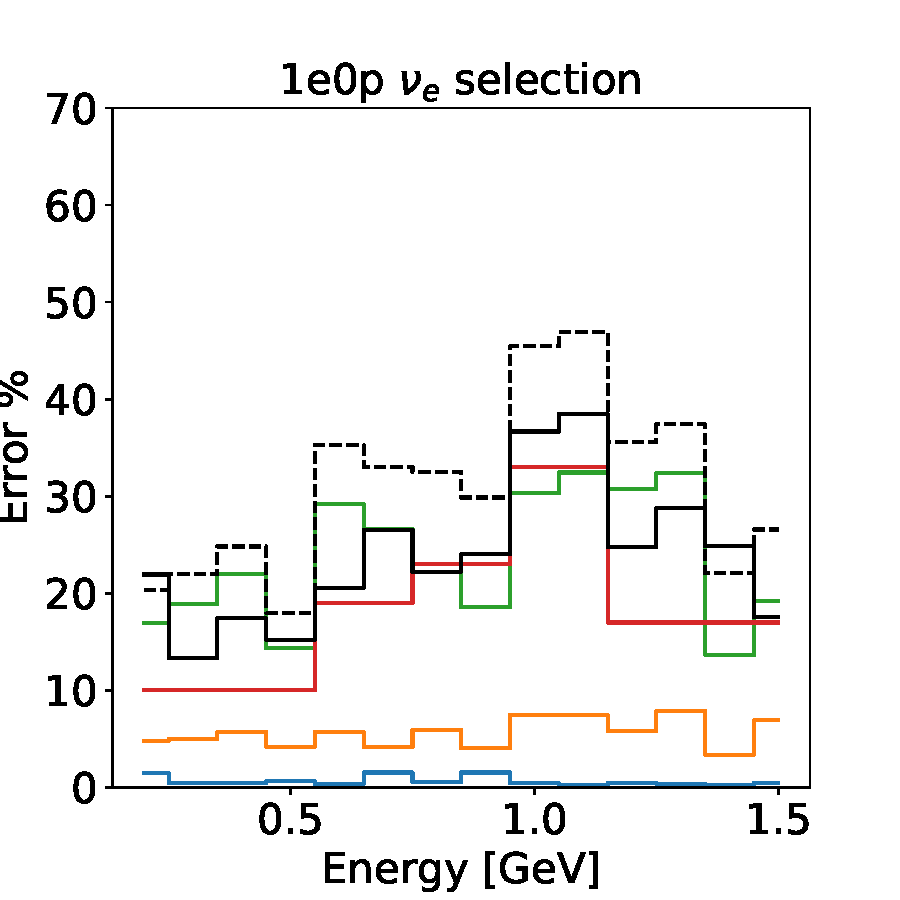
\includegraphics[width=1.00\textwidth]{Systematics/1e0p_syst_summary.pdf}
    \caption{\label{fig:systsummary:zp}\zpsel}
    \end{subfigure}
    \begin{subfigure}[b]{0.32\textwidth}
    \centering
    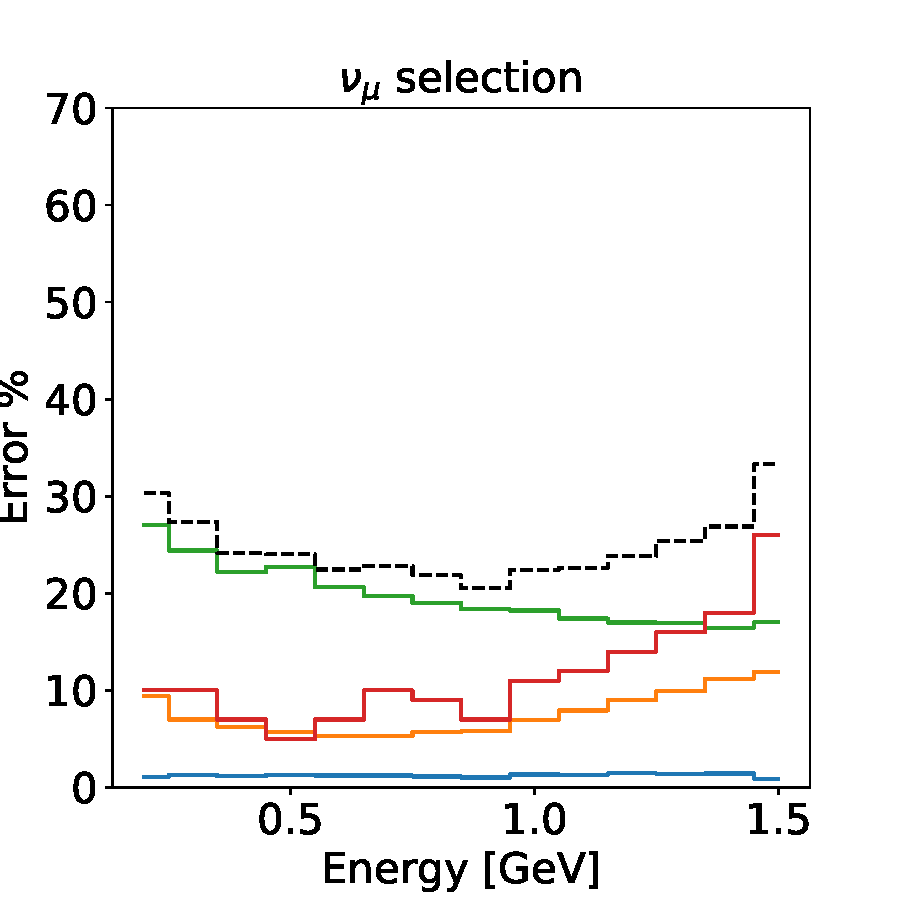
\includegraphics[width=1.00\textwidth]{Systematics/numu_syst_summary.pdf}
    \caption{\label{fig:systsummary:numu}\numu}
    \end{subfigure}
\caption{\label{fig:systsummary}Summary of systematic errors on the analysis.}
\end{center}
\end{figure}

\subsection{Detector Systematics}
\label{sec:detsys}
\par This section discusses both the impact and the treatment of detector systematics in the analysis. Details on MicroBooNE's approach to handling detector systematics can be found in~\cite{bib:detsyssupportnote}. 
\begin{enumerate}
    \item Waveform variations in the examined variables ($x$, $yz$, $\theta_{XZ}$, $\theta_{YZ}$, $dE/dx$). These detector variations are constructed by profiling reconstructed hit variables of charge, amplitude and width as a function of the mentioned variables with data-driven samples, and re-scaling the simulation by the difference between data and simulation. By doing this, the samples cover the difference between data and simulation by construction. 
    \item Light response variations to estimate the light yield (LY) simulation uncertainty. Three variations are envisioned: (1) 25\% uniform drop in LY to account for mis-modeling of the absolute LY in the detector. (2) 120 cm (compared to the simulation's 60 cm) Rayleigh scattering length and (3) 8 meter light attenuation length to account for drift-distance dependent mis-modeling.
    \item Space-Charge variation sample constructed by using an alternative E-field map produced relying more heavily on cosmic muons rather than laser calibration runs. The coverage of the two maps is stronger in different regions of the detector, and the differences between them are believed to cover uncertainties in our E-field mapping. 
    \item Recombination specific variation, built by using a variation of the input parameters to the Modified Box model which are meant to cover the data/mc differences observed at high \dedx for protons in MCC8 analyses. This variation is redundant with respect to the wire-modification \dedx variation, but used as a cross-check. 
\end{enumerate}
\par Detector systematics samples are generated as \emph{uni-sim} variations, meaning that, for each detector effect, a given MC event is re-simulated once with a change to a detector modeling parameter. This produces a new simulation of the same underlying neutrino interactions, which can be used to measure the impact of the detector effect being studied on efficiencies, reconstructed variables, and event pass-rates, factoring out statistical fluctuations.
\par In the context of a sensitivity calculation, detector systematics unisims can be used to calculate a covariance matrix for selected event rates in each bin used in the sensitivity calculation. Only diagonal elements of the covariance matrix are then added to the total uncertainty matrix. 
The main drawback of this approach is the fact that the excursion in the number of measured events in a bin computed from a single variation is taken as the 1$\sigma$ excursion for the error estimation.
\par Sections~\ref{sec:detsys:light},~\ref{sec:detsys:tpc}, and~\ref{sec:detsys:datamc} below summarize the impact that important detector variations have on the analysis in terms of selection efficiencies and reconstructed variable smearing. They are supplemented by several focused presentations described in DocDBs~\href{https://microboone-docdb.fnal.gov/cgi-bin/private/ShowDocument?docid=30373}{30373}, ~\href{https://microboone-docdb.fnal.gov/cgi-bin/private/ShowDocument?docid=30022}{30022},~\href{https://microboone-docdb.fnal.gov/cgi-bin/private/ShowDocument?docid=29938}{DocDB 29938}, and~\href{https://microboone-docdb.fnal.gov/cgi-bin/private/ShowDocument?docid=29299}{29299}. Section~\ref{sec:detsys:selections} presents the quantitative estimation of detector systematics on the \nue and \numu selections which re then fed as input to SBNFit for the constraint and sensitivity calculation.
%\par Below, simple comparisons of distributions relevant to the analysis under different detector variation samples are shown, but the full inclusion of detector systematics in the sensitivity calculation has not been performed. For calorimetric variables such as electron \dedx and $\pi^0$ mass some clear differences, such as shifts in energy scale, are visible, though contained to within a few percent. These initial comparisons are promising in that they seem to suggest a relatively minor impact to the analysis from detector systematics. 

\subsubsection{Impact of Light Modeling on Neutrino ID and Cosmic Rejection} 
\label{sec:detsys:light}
The \texttt{SliceID} (sec.~\ref{sec:sliceID}) tools used to isolate and identify neutrino interactions in each event rely on scintillation light to identify interactions in-time with the beam and thus likely neutrino candidates. The tools developed aim to reject TPC interactions that are incompatible with the in-time optical flash, rather than selecting the most compatible TPC interaction. This allows the \texttt{SliceID} to rely on light information in a conservative manner, and allows the analysis to be impacted minimally by the significant light mismodeling and time-dependence in scintillation light response observed in the detector. 
\par Two variations are used to cover overall light mis-modeling: one accounts for a 25\% lower light-yield across the detector (25 \% LY) and another for the uncertainty in the Rayleigh scattering length, simulated at 60 cm in MicroBooNE's CV and varied to 120 cm in the systematic variation sample. A third variation, specific to Run3 and beyond, accounts for mis-modling in the calibration applied to account for time-dependent light degradation in the detector. The effect these variations have on reconstructed light variables used in the analysis is documented in~\href{https://microboone-docdb.fnal.gov/cgi-bin/private/ShowDocument?docid=29299}{DocDB 29299}.

\par The impact of these significant variations on the \texttt{SliceID} performance is shown in figure~\ref{fig:detsys:light:eff}. The level of variation in efficiency observed is quite small, with larger variations focused on the 200-300 MeV energy bin for $\nu_{\mu}$ interactions.


\begin{figure}[H] 
\begin{center}
    \begin{subfigure}[b]{0.45\textwidth}
    \centering
    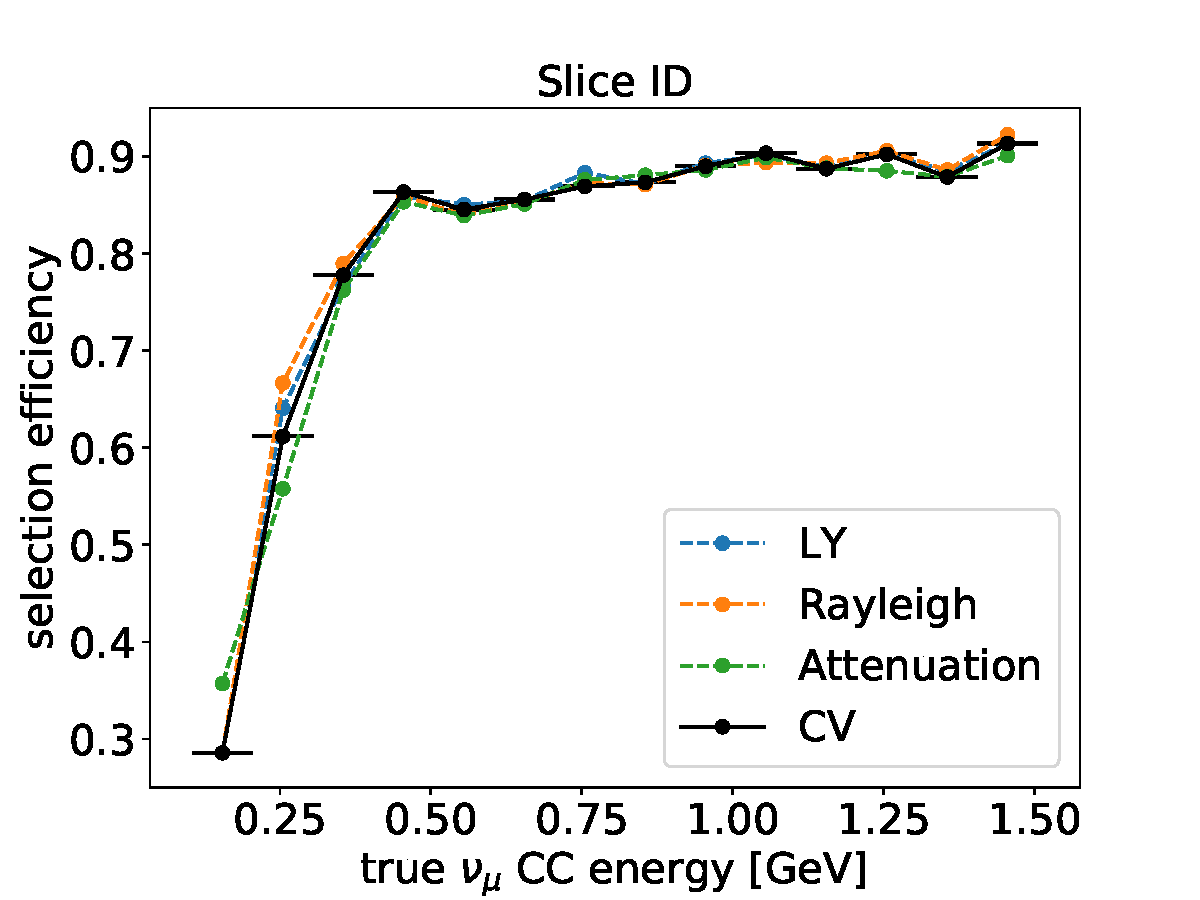
\includegraphics[width=1.00\textwidth]{detsys/light/nu_e_03232020_eff_light_numu.pdf}
    \caption{\label{fig:detsys:light:eff:numu}SliceID on $\nu_{\mu}$}
    \end{subfigure}
    \begin{subfigure}[b]{0.45\textwidth}
    \centering
    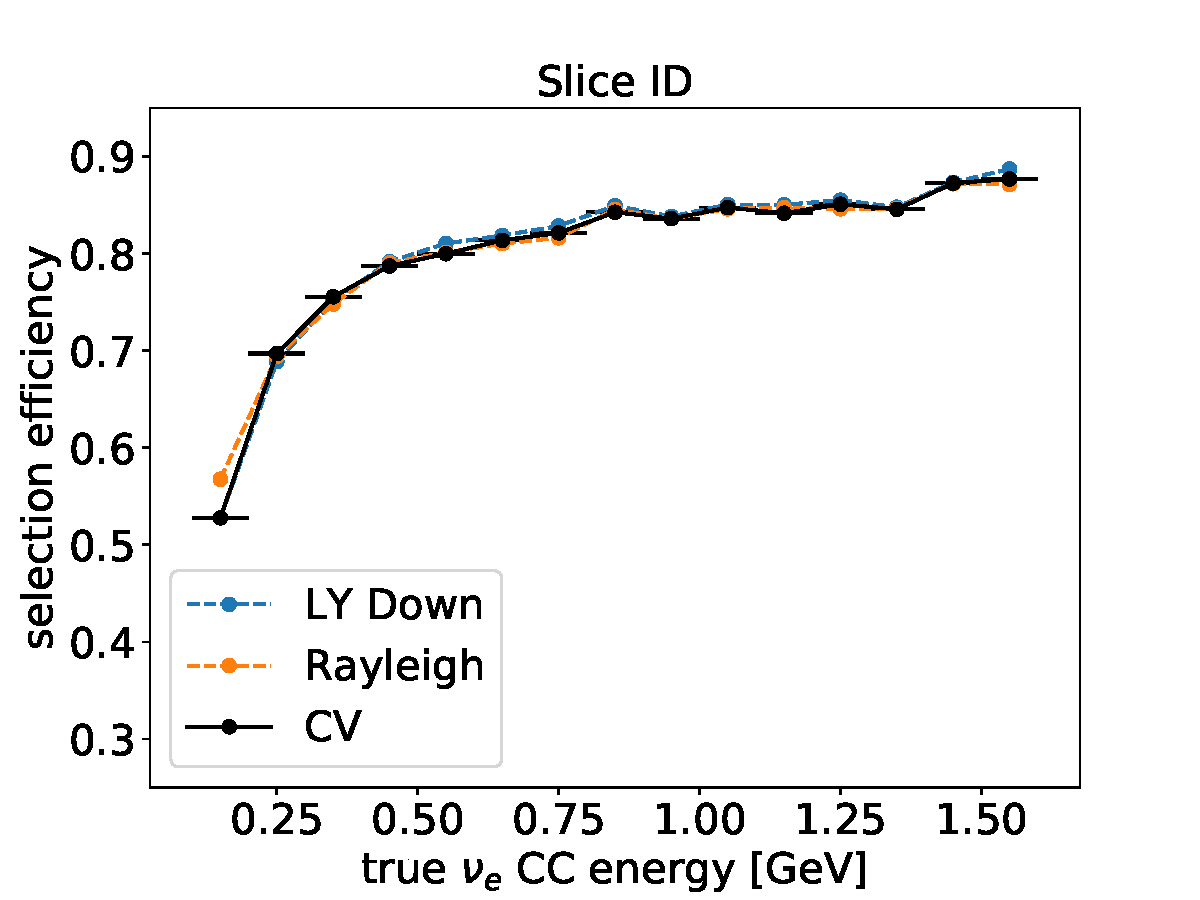
\includegraphics[width=1.00\textwidth]{detsys/light/nu_e_03232020_eff_light_nue.pdf}
    \caption{\label{fig:detsys:light:eff:nue}SliceID on $\nu_{e}$}
    \end{subfigure}
\caption{\label{fig:detsys:light:eff}Impact of light variations on SliceID efficiency for $\nu_{\mu}$ and $\nu_e$ events.}
\end{center}
\end{figure}
\par It is important to note that while the light variations being considered as input to measure the impact of detector systemtatics are substantial, they do not fully cover the data-mc differences in the \textit{flash-PE} variable (which measures the integrated prompt plus late light produced in time with the neutrino beam) at low PE. This can be seen in slide 12 of~\href{https://microboone-docdb.fnal.gov/cgi-bin/private/ShowDocument?docid=29299}{DocDB 29299}. While the robustness of the analysis against light variation is an inherent design of the \texttt{SliceID}~\ref{sec:sliceID}, we further validate susceptibility to light-mismodeling by studying the time-dependence of the neutrino selection tools as a function of reconstructed $x$ position (which impacts light yield considerably). No noticeable change in performance is observed over time.

\begin{figure}[hbt!] 
\begin{center}
    \begin{subfigure}[b]{0.3\textwidth}
    \centering
    %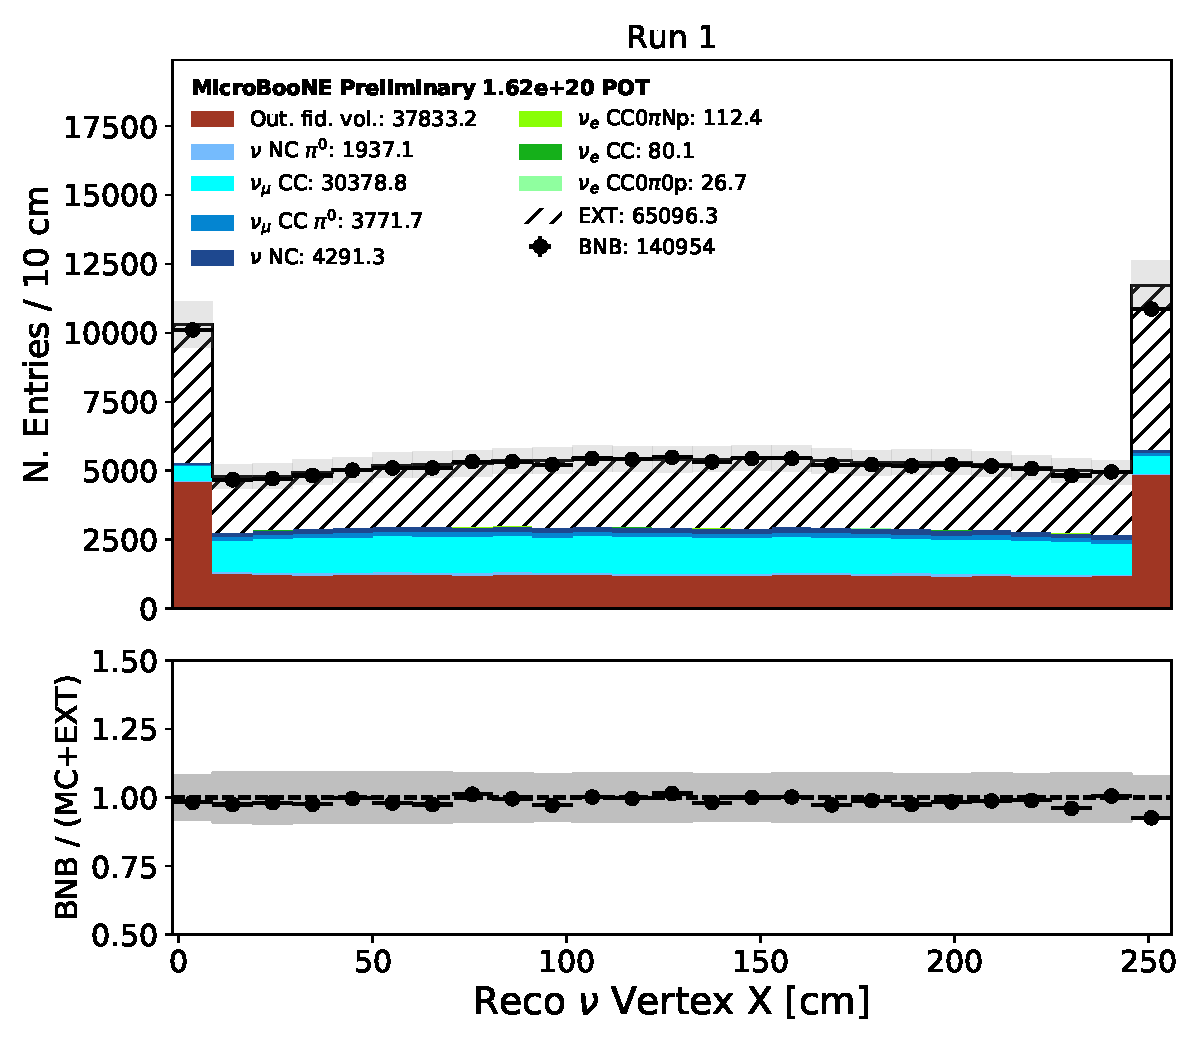
\includegraphics[width=1.00\textwidth]{NuMuCCsel/Images/Ryan/Run1/reco_nu_vtx_sce_x_08062020_samples_longest_noCRT_event_category.pdf}
    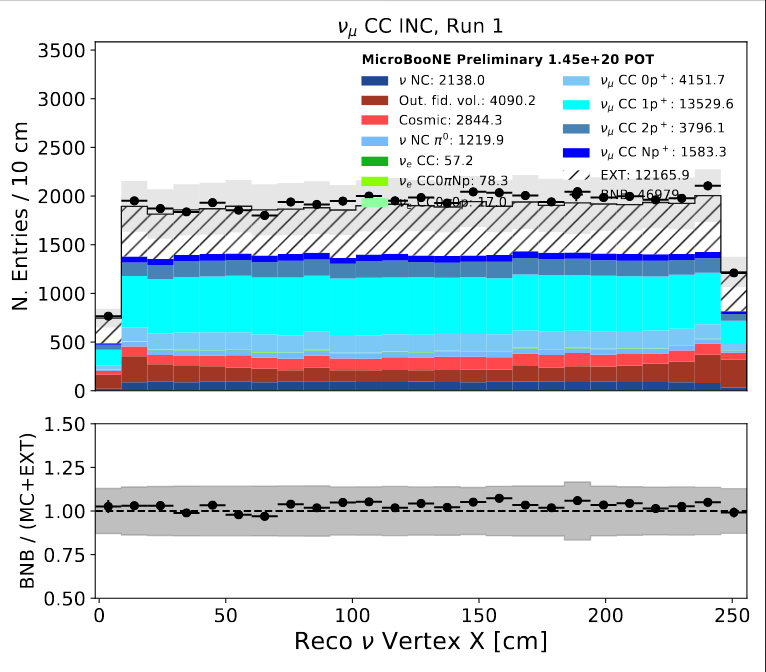
\includegraphics[width=1.00\textwidth]{detsys/light/vtx_x_1.png}
    \caption{\label{fig:systematics:run1:nuvtxx}vertex $x$ - Run 1}
    \end{subfigure}
    \begin{subfigure}[b]{0.3\textwidth}
    \centering
    %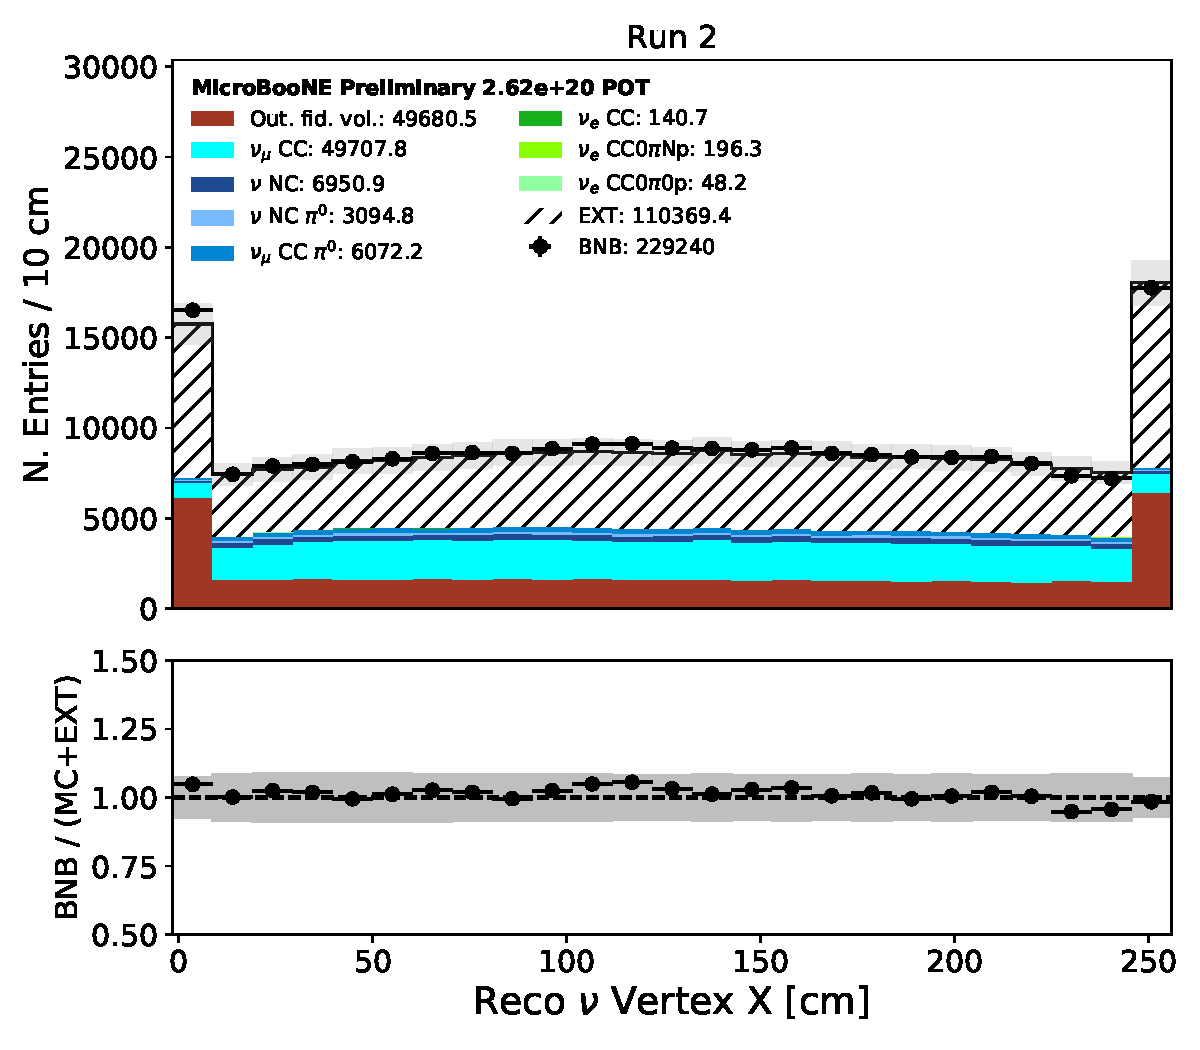
\includegraphics[width=1.00\textwidth]{NuMuCCsel/Images/Ryan/Run2/reco_nu_vtx_sce_x_08062020_samples_longest_noCRT_event_category.pdf}
    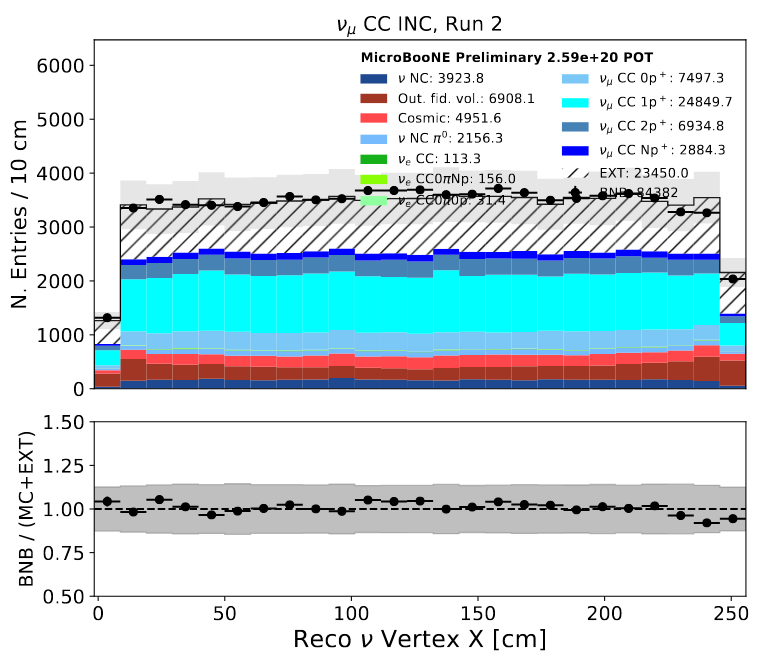
\includegraphics[width=1.00\textwidth]{detsys/light/vtx_x_2.png}
    \caption{\label{fig:systematics:run2:nuvtxx}vertex $x$ - Run 2}
    \end{subfigure} %\newline
    \begin{subfigure}[b]{0.3\textwidth}
    \centering
    %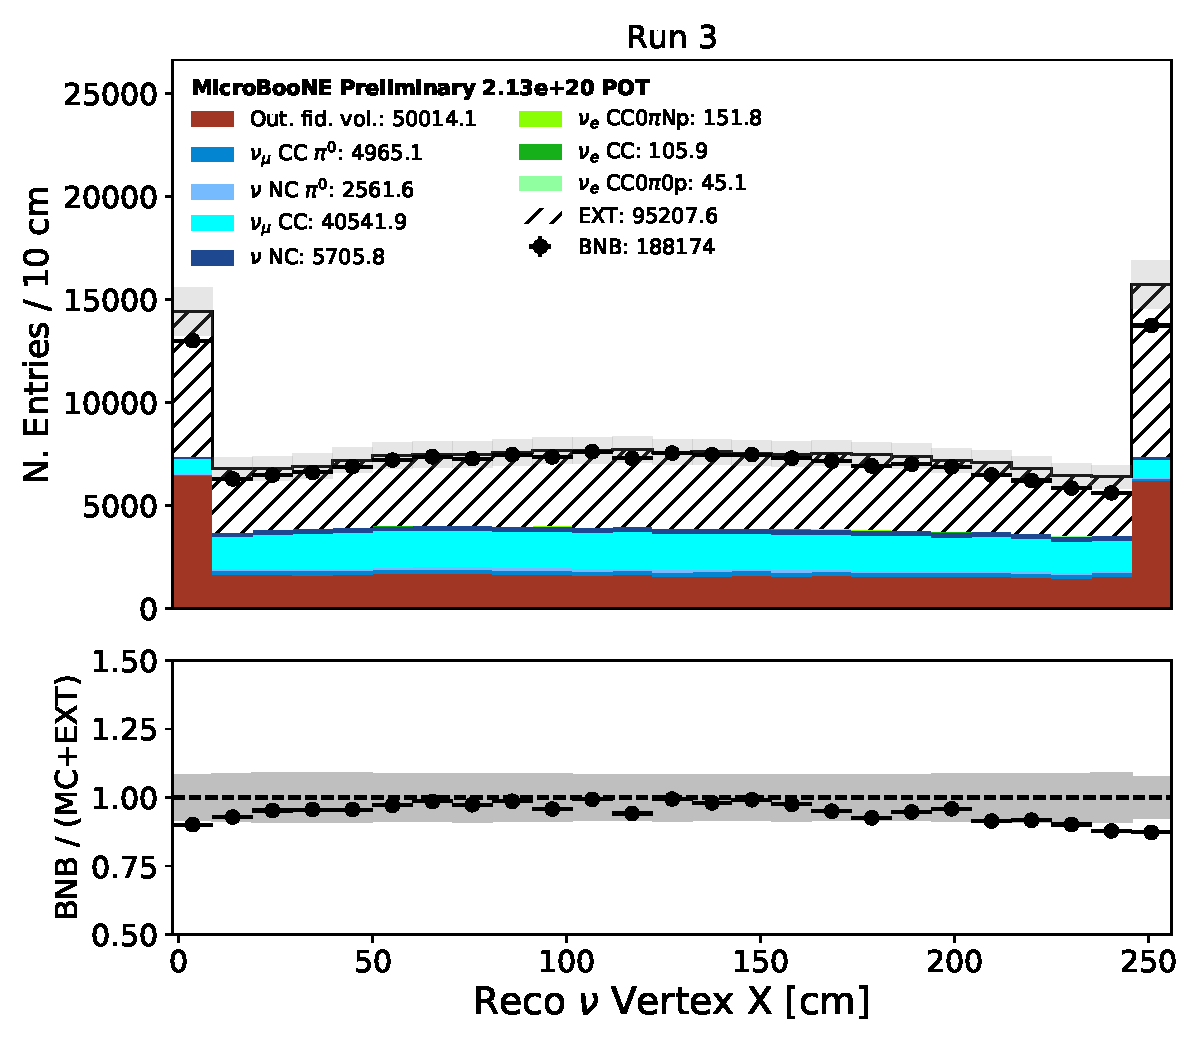
\includegraphics[width=1.00\textwidth]{NuMuCCsel/Images/Ryan/Run3_nocrt/reco_nu_vtx_sce_x_08062020_samples_longest_noCRT_event_category.pdf}
    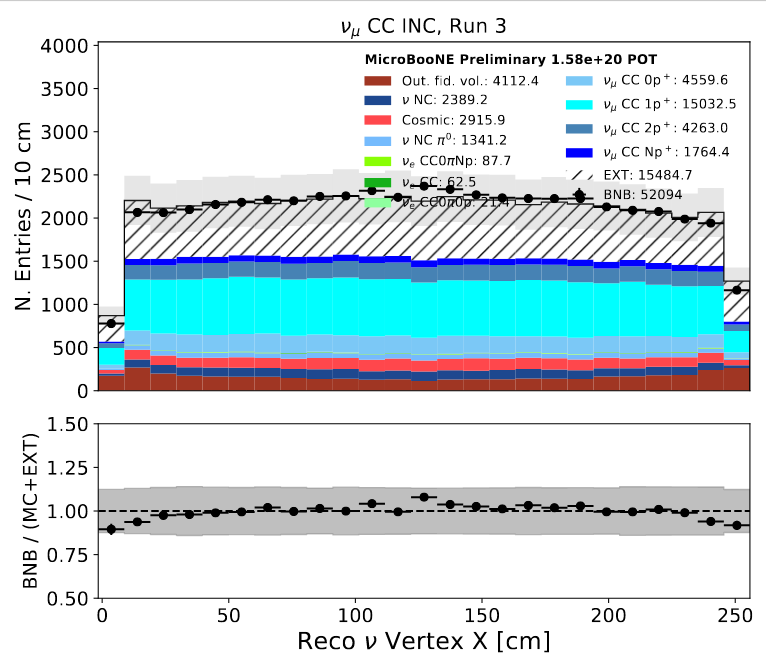
\includegraphics[width=1.00\textwidth]{detsys/light/vtx_x_3.png}
    \caption{\label{fig:systematics:run3:nuvtxx}vertex $x$ - Run 3}
    \end{subfigure}
\caption{X coordinates of reconstructed neutrino vertex for each run. SliceID applied.}
\label{fig:systematics:numu:nuvtxx}
\end{center}
\end{figure}

\subsubsection{Systematics on Energy Scale and Particle ID} 
\label{sec:detsys:tpc}
Systematics which impact the TPC's response can impact calorimetric energy reconstruction important for shower and thus $\nu_e$ event energy reconstruction. Impact on range-based track energy is also expected, though to a lesser extent, and largely confined to systematics related to SCE position reconstruction. This section studies the impact of simulation uncertainties on energy scale reconstruction.
\par The impact of different variation samples on shower energy scale are studied by measuring the variation of the reconstructed $M_{\gamma\gamma}$ for selected $\pi^0$ candidate events. The outcome of these studies is summarized in table~\ref{tab:energyvar}. More details describing these studies is available in ~\href{https://microboone-docdb.fnal.gov/cgi-bin/private/ShowDocument?docid=29299}{DocDB 29299}.


\begin{table}[H]
\centering
\setlength{\tabcolsep}{10pt}
\renewcommand{\arraystretch}{1.25}
 \begin{tabular}{| c | c | c | c | c |} 
 \hline
 variation & $M_{\pi^0}$ bias [\%] & $M_{\pi^0}$ smearing [\%] & $p$ KE bias [\%] & $p$ KE smearing [\%]  \\
 \hline
WireMod X & -2.5 & 0.7 & 0.0 & $<$ 0.1 \\
WireMod YZ & +0.4 & 2.1 & 0.0 & $<$ 0.1 \\
WireMod Angle XZ & +0.3 & 0.3 & 0.0 & $<$ 0.1 \\
WireMod Angle YZ & +2.4 & 0.3 & 0.0 & $<$ 0.1 \\
Space Charge & N.A. & N.A. & 0.0 & $<$ 0.4 \\
 \hline
 \end{tabular}
 \caption{\label{tab:energyvar} Impact of TPC detector systematic variations on reconstructed calorimetric shower energy and range-based proton energy. The impact of these systematics is rather contained, generally at the percent or sub-percent level.}
\end{table}


TPC variations which impact spatial and calorimetric reconstruction can impact particle ID discriminant variables such as the \texttt{LLR trkpid} used for $\mu$/$p$ separation and \dedx used for $e$/$\gamma$ separation. Studies specific to the impact of detector variations on PID reconstructed quantities are described in DocDBs~\href{https://microboone-docdb.fnal.gov/cgi-bin/private/ShowDocument?docid=31444}{31444} and~\href{https://microboone-docdb.fnal.gov/cgi-bin/private/ShowDocument?docid=29070}{29070}. These are summarized by the impact that the variations have on the selection efficiency for protons and electrons spectively, calculated with the cuts as defined in the \npsel Box-Cut selection. The impact overall is small and contained to a few percent variation, as shown in figure~\ref{fig:syst:detsys:pid}.

\begin{figure}[H] 
\begin{center}
    \begin{subfigure}[b]{0.4\textwidth}
    \centering
    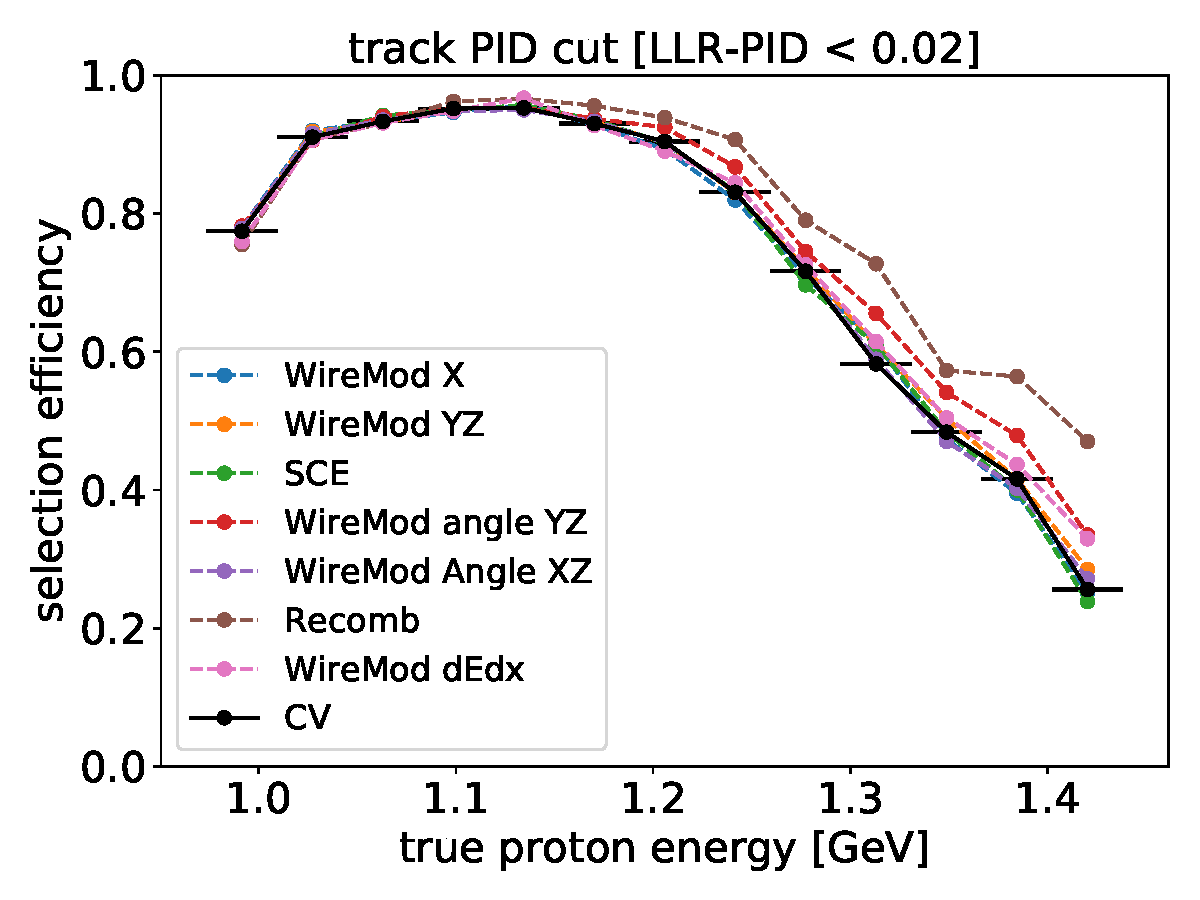
\includegraphics[width=1.00\textwidth]{detsys/PID/proton_e_03292020_eff_trkpid_nues.pdf}
    \caption{\label{fig:detsys:pid:proton} Proton PID eff. variation}
    \end{subfigure}
    \begin{subfigure}[b]{0.4\textwidth}
    \centering
    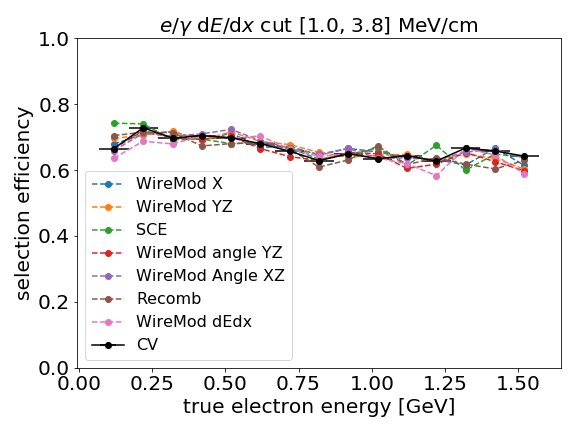
\includegraphics[width=1.00\textwidth]{detsys/PID/elec_e_03312020_eff_11_nue_pdf.png}
    \caption{\label{fig:detsys:pid:electron}Electron PID eff. variation}
    \end{subfigure}
\caption{\label{fig:syst:detsys:pid}Impact of TPC detector variations (after \npsel pre-selection) on proton and electron PID cuts in \npsel box-cuts. Left, cut on track PID for true backtracked protons. Right: cut on \dedx for true backtracked electrons.}
\end{center}
\end{figure}

\subsubsection{Validation of Detector Systematic Coverage of Detector Uncertainties}
\label{sec:detsys:datamc}
\par This section presents key distributions with the inclusion of detector systematics to understand if the detector systematics samples employed are sufficient to cover discrepancies observed in detector modeling. We focus on distributions that are relevant to understanding detector modeling and that are most impactful for the analysis' performance. Additional data-mc comparisons are included in ~\href{https://microboone-docdb.fnal.gov/cgi-bin/private/ShowDocument?docid=29299}{DocDB 29299}.
%\par For light modeling, we focus on the distribution of \texttt{flash PE} after the Slice ID and a basic fiducialization cut of neutrino candidates. The distribution is shown for Run1 in figure~\ref{fig:detsys:datamc:flashpe:run1} and for Run3 in figure~\ref{fig:detsys:datamc:flashpe:run3}. On the left hand side, only statistical errors re include, and a significant discrepancy in data-MC is evident. On the right hand side, the same comparison including detector systematics are included. For Run1 these include a 25\% LY quenching and the Rayleigh scattering variation. For Run3 the modeling of x-dependent attenuation is also included. While the systematics cover a significant amount of the data-mc differences, they do not cover the full discrepancy, especially at low PE.
\par First we show the distributions of $M_{\gamma\gamma}$ and \dedx from $\pi^0$ candidate events, produced using $6.78e20$ POT of BNB data. 
The plots show the distributions with statistical errors only plus all detector systematics. No flux, crss-section, or re-interaction systematics are included in this area-normalized data/mc comparison. Detector systematics are computed using the relevant variations from CC $\pi^0$ monte-carlo and calculating the fractional event variation in each relevant distribution. This fractional error, bin-by-bin, is applied as an additional uncertainty and summed in quadrature to statistical errors for all the MC contributions in the plot. These studies indicate that current TPC systematics do a good job covering the level of discrepancy observed in relevant data-mc comparisons. In particular, we see tht the $M_{\gamma\gamma}$, showing good agreement out of the box, is subject to small detector uncertainties, while the \dedx distribution which shows  a clear shift in the peak at 4 MeV/cm presents a significant uncertainty which covers this discrepancy. We are confident given these studies that detector uncertainties on shower kinematics and variables are adequately covered in the analysis.

\begin{figure}[H] 
\begin{center}
    \begin{subfigure}[b]{0.4\textwidth}
    \centering
    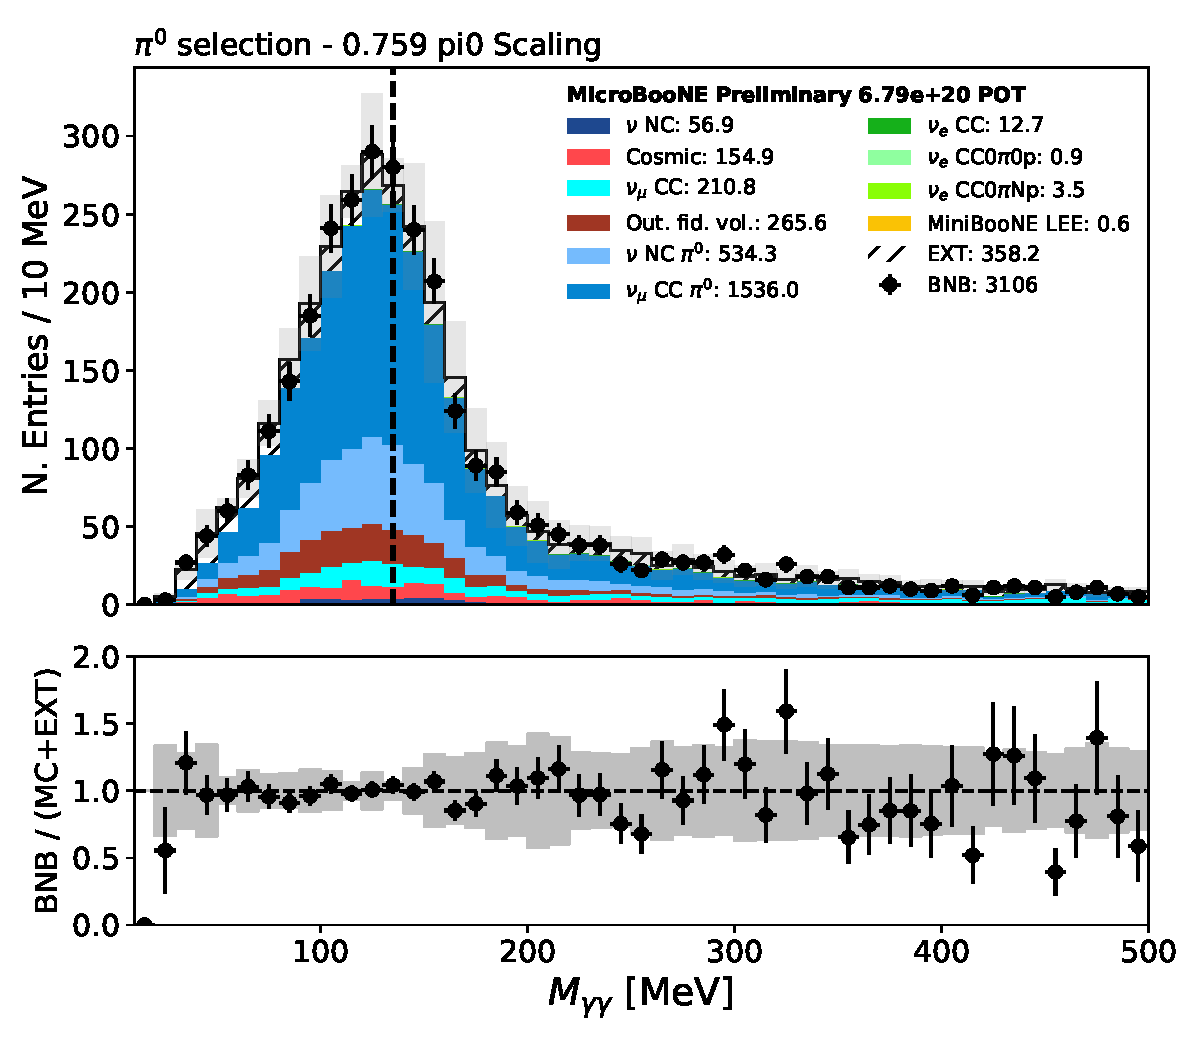
\includegraphics[width=1.00\textwidth]{detsys/datamc/pi0_mass_Y_corr_run123.pdf}
    \caption{\label{fig:detsys:datamc:pi0mass} $\pi^0$ mass}
    \end{subfigure}
    \begin{subfigure}[b]{0.4\textwidth}
    \centering
    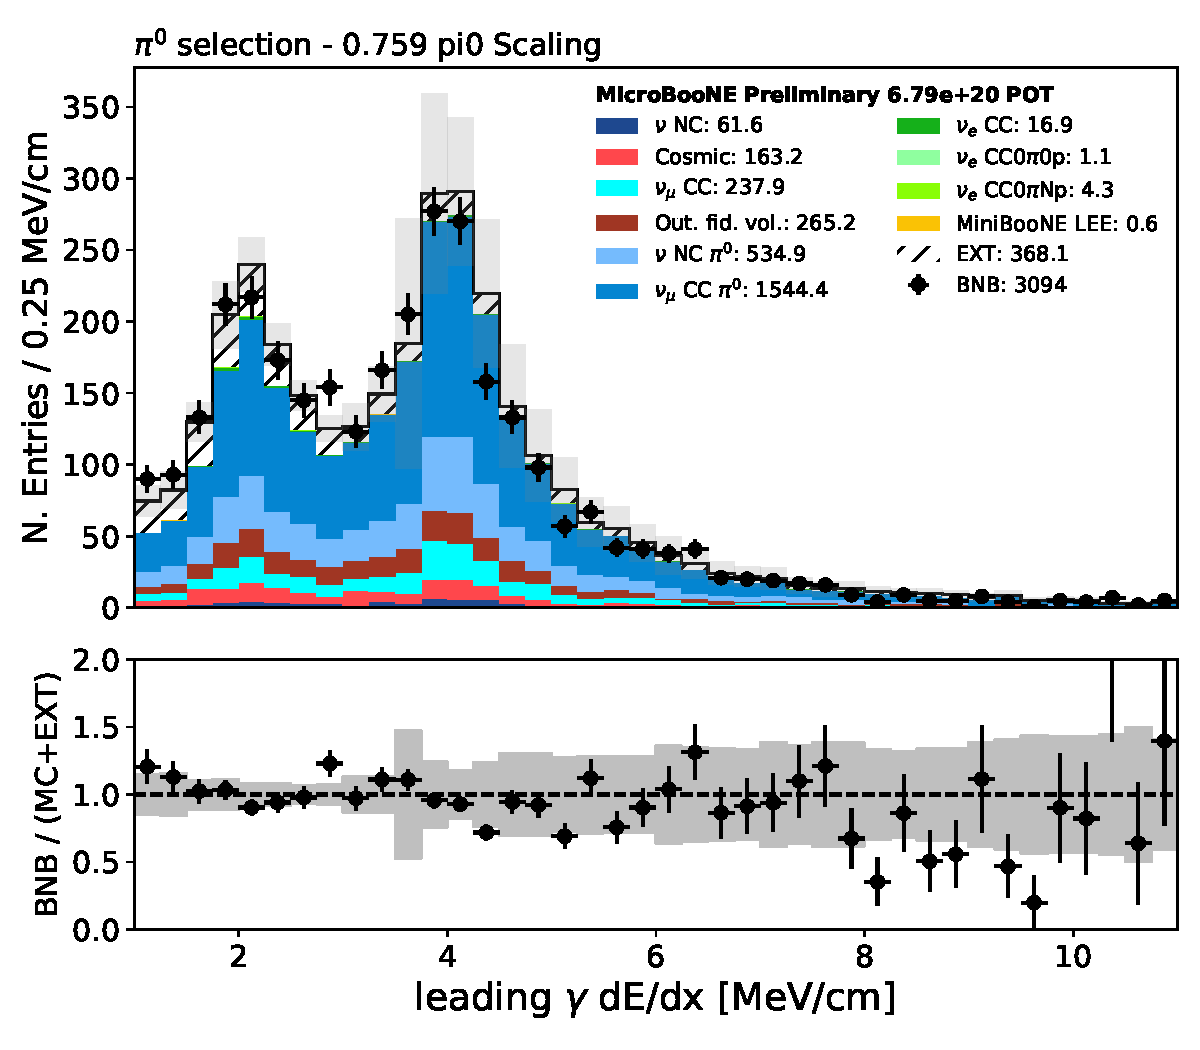
\includegraphics[width=1.00\textwidth]{detsys/datamc/pi0_dedx1_fit_Y_run123.pdf}
    \caption{\label{fig:detsys:datamc:pi0dedx}leading $\gamma$ \dedx}
    \end{subfigure}
\caption{\label{fig:detsys:datamc:dedx} area-normalized $\pi^0$ mass and \dedx distributions from the $\pi^0$ sideband with statistical plus detector systematic errors. The mass distribution has a $\chi^2$ of 52.3/48 and 14.4/48 before/after the inclusion of detector systematics, corresponding to p-values of 0.31 and 1.00 respectively. For the \dedx distribution these values are 89.9/40 and 16.9/40 translating to 0.00 and 1.00 respectively.}
\end{center}
\end{figure}

\begin{comment}
\begin{figure}[H] 
\begin{center}
    \begin{subfigure}[b]{0.4\textwidth}
    \centering
    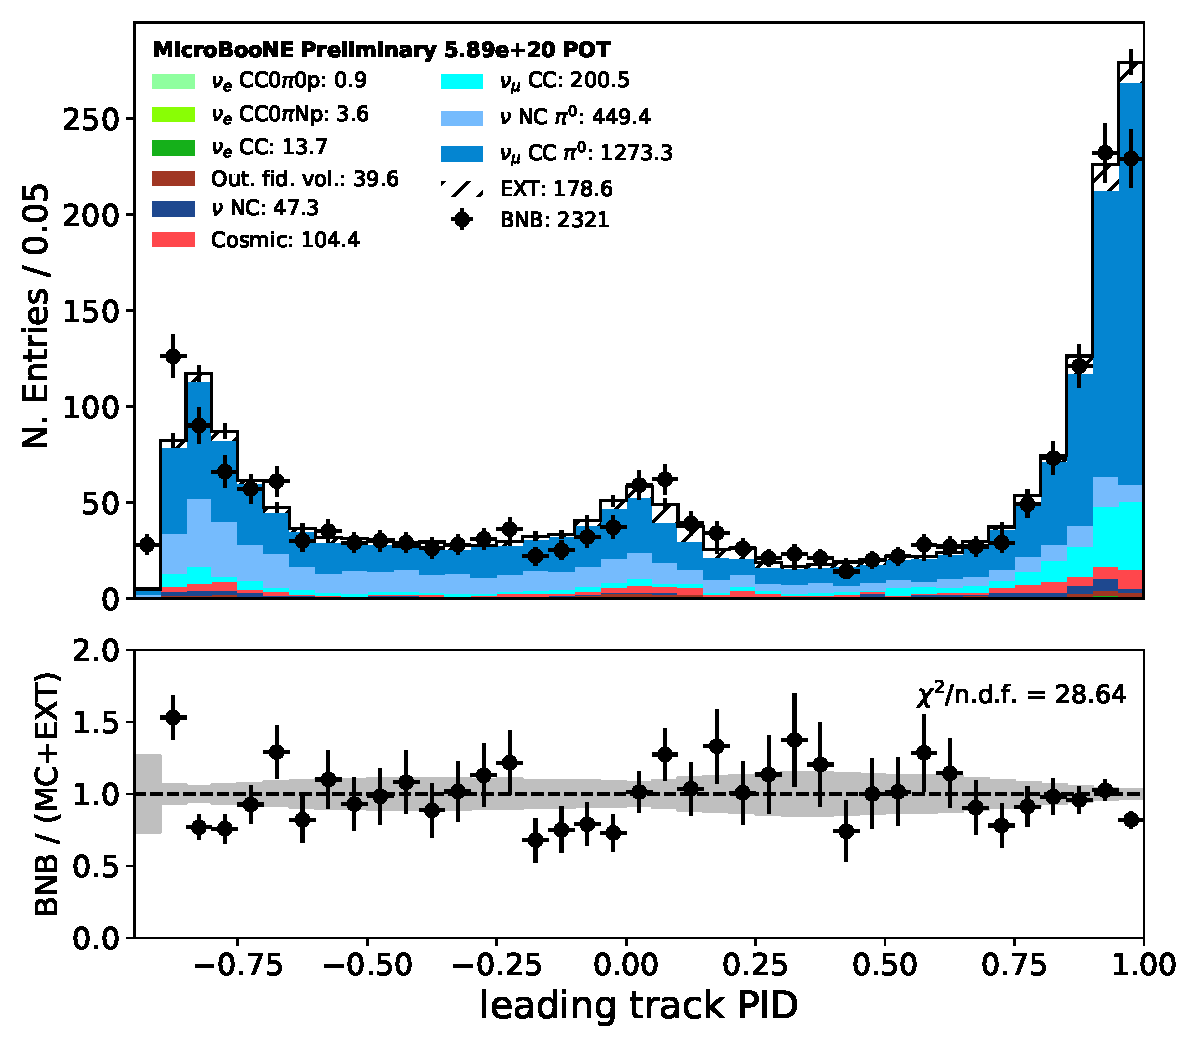
\includegraphics[width=1.00\textwidth]{detsys/datamc/trkpid_03292020_statonly.pdf}
    \caption{\label{fig:detsys:datamc:trkpid:stat} stat-only}
    \end{subfigure}
    \begin{subfigure}[b]{0.4\textwidth}
    \centering
    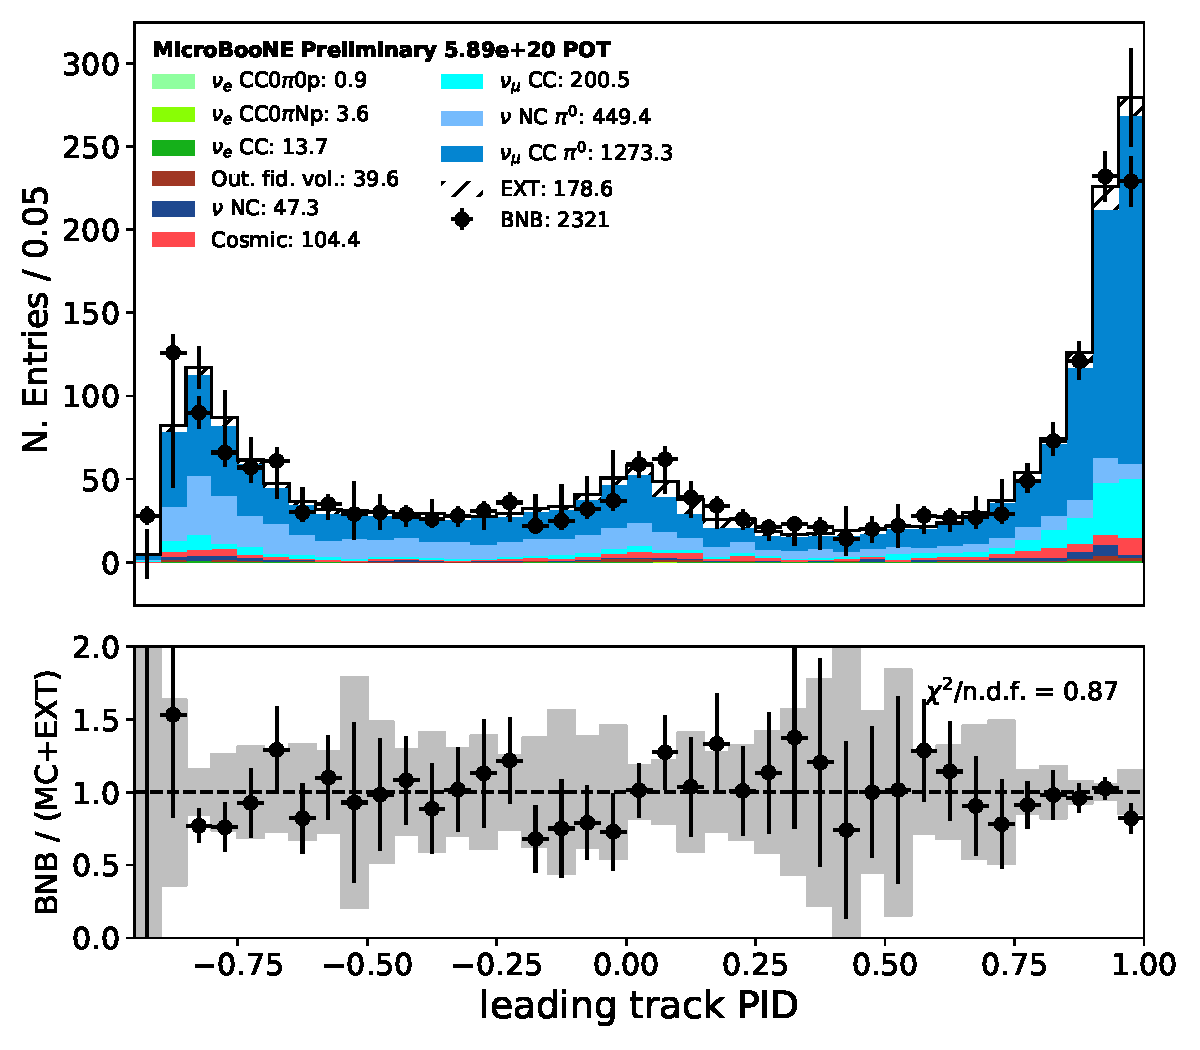
\includegraphics[width=1.00\textwidth]{detsys/datamc/trkpid_03292020_detsys.pdf}
    \caption{\label{fig:detsys:datamc:trkpid:all}All Wire-Mod}
    \end{subfigure}
\caption{\label{fig:detsys:datamc:trkpid}Track PID score for longest track in selected $\pi^0$ candidate events without (left) and with (right) wire-modification detector systematics.}
\end{center}
\end{figure}
\end{comment}


In order to better study the data/simulation discrepancies in calorimetric reconstruction for tracks, the selection of contained protons shown in section \ref{sec:sideband:stopping_muons_protons} has been used, comparing the data with the central value and with the WireMod \dedx variation sample, to test in particular the impact of recombination uncertainties.
The two plots in figure \ref{fig:syst:dedx_1d} show an example of the comparison of the \dqdx distribution, performed in bins of residual range and pitch, differently for every plane.
The discrepancy between the data and the central value of the simulation is significantly corrected after applying the WireMod \dedx variation.
The entire set of comparisons in every bin of residual range and pitch is available in \cite{bib:pid_internal_note}.

\begin{figure}[H] 
\begin{center}
    \begin{subfigure}[b]{0.4\textwidth}
    \centering
    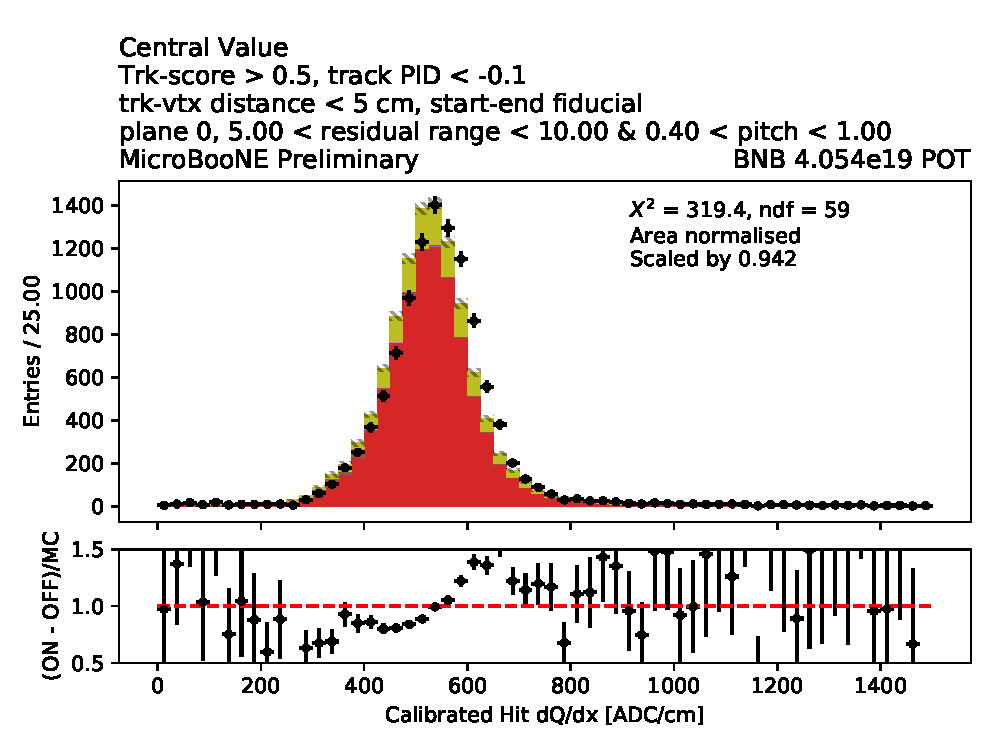
\includegraphics[width=1.00\textwidth]{detsys/calorimetry_dqdx/bnb_nu_mod_0005_rr_0010_004_pitch_010_noleg.pdf}
    \caption{\label{fig:syst:dedx_1d:cv} Central value.}
    \end{subfigure}
    \begin{subfigure}[b]{0.4\textwidth}
    \centering
    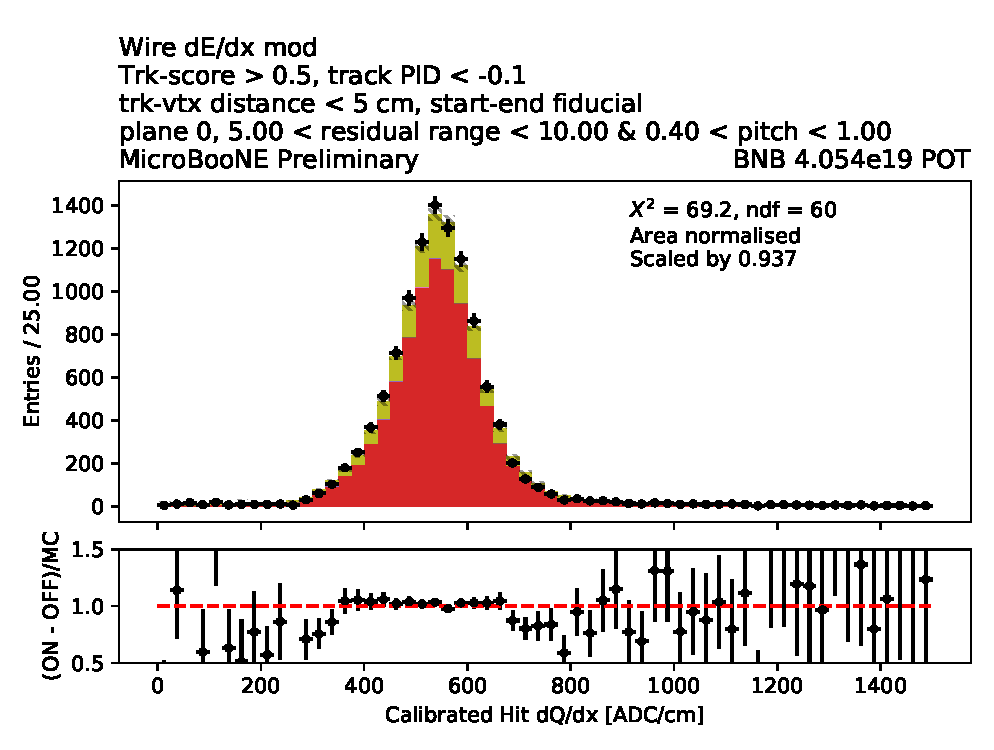
\includegraphics[width=1.00\textwidth]{detsys/calorimetry_dqdx/bnb_nu_wire_dedx_mod_0005_rr_0010_004_pitch_010_noleg.pdf}
    \caption{\label{fig:syst:dedx_1d:wiremod_dedx} WireMod \dedx variation.}
    \end{subfigure}
\caption{\label{fig:syst:dedx_1d}The WireMod \dedx sample improves the accuracy of the simulation with respect to the central value in the \dqdx distribution. 
Here is shown one example of the relevant data/simulation comparison, for a given bin of residual range and pitch, on the first induction plane, using the contained proton selection described in section \ref{sec:sideband:stopping_muons_protons}
The red component of the histogram corresponds to proton hits, while the brown to neutrino-induced muons and the yellow to cosmic-induced tracks.}
\end{center}
\end{figure}

The three plots in figure \ref{fig:syst:dedx_vs_rr} summarise the information displayed in the \dqdx data/simulation comparison, by showing a 2-dimensional histogram of \dqdx and residual range, for the data, the central value of the simulation, and the WireMod \dedx sample.
In order to reduce possible biases due to the underlying distributions, these histograms are produced in bins of pitch, and they are normalised as estimates of p(\dqdx|residual range), rather than p(\dqdx, residual range).
This ensures that the probability of every vertical slice sums up to unity, making it less sensitive to the underlying distribution of the track length.
The curve showing the theoretical most probable value is superimposed over the histogram to facilitate the comparison between the data and the simulation.
%It is important to keep in mind that what matters for the analysis is the agreement between the data and the simulation, and not the agreement between the data and the theoretical curve, or between the simulation and the theoretical curve.
The qualitative conclusion derived earlier, i.e. that the WireMod \dedx sample improves the accuracy of the simulation, remains unchanged even after looking these 2-dimensional plots. These studies also given an indication that the analysis is roust against \dedx mis-modeling.

\begin{figure}[H] 
\begin{center}
    \begin{subfigure}[b]{0.32\textwidth}
    \centering
    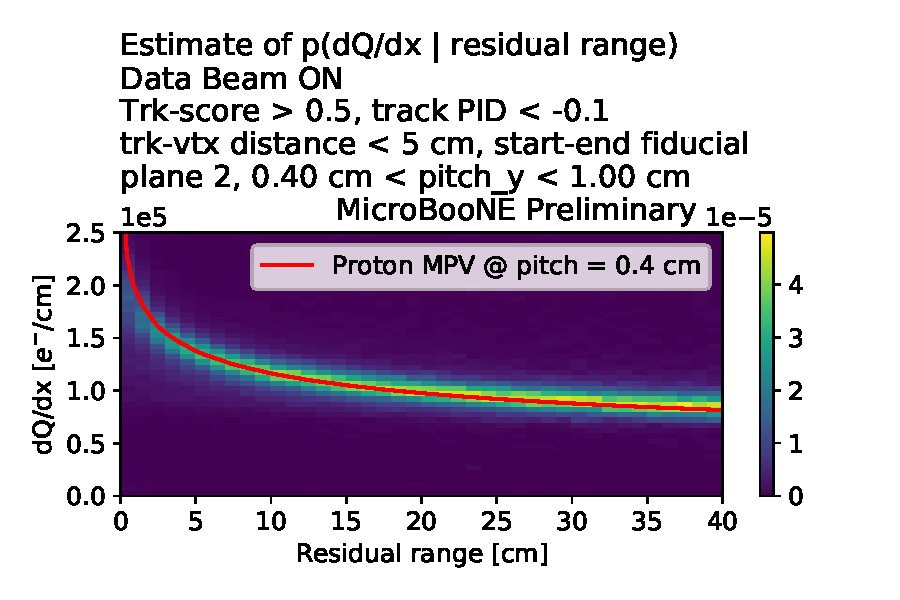
\includegraphics[width=1.00\textwidth]{detsys/calorimetry_dqdx/beam_on_04_pitch_y_10.pdf}
    \caption{\label{fig:syst:dedx_vs_rr:data} Data.}
    \end{subfigure}
    \begin{subfigure}[b]{0.32\textwidth}
    \centering
    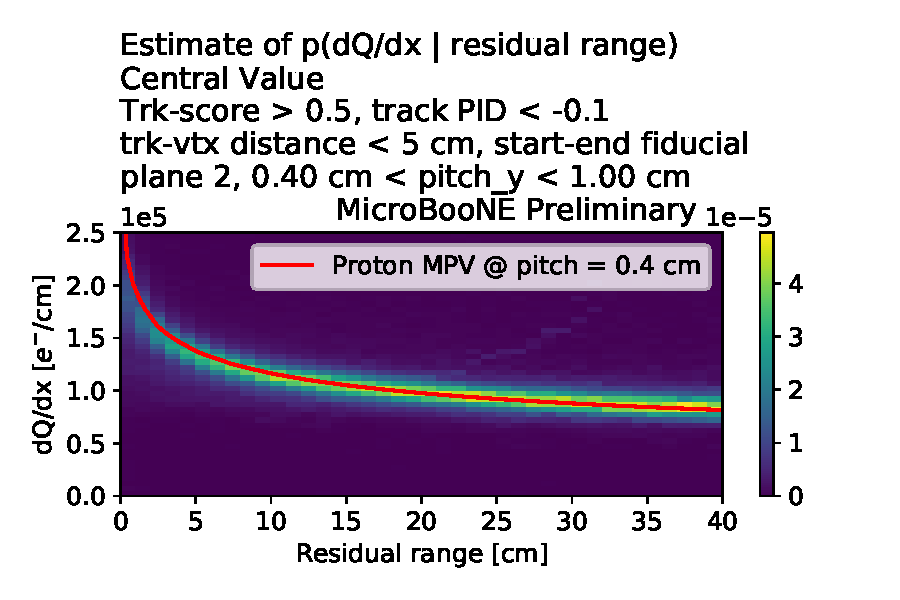
\includegraphics[width=1.00\textwidth]{detsys/calorimetry_dqdx/bnb_nu_mod_04_pitch_y_10.pdf}
    \caption{\label{fig:syst:dedx_vs_rr:cv} Simulation central value.}
    \end{subfigure}
    \begin{subfigure}[b]{0.32\textwidth}
    \centering
    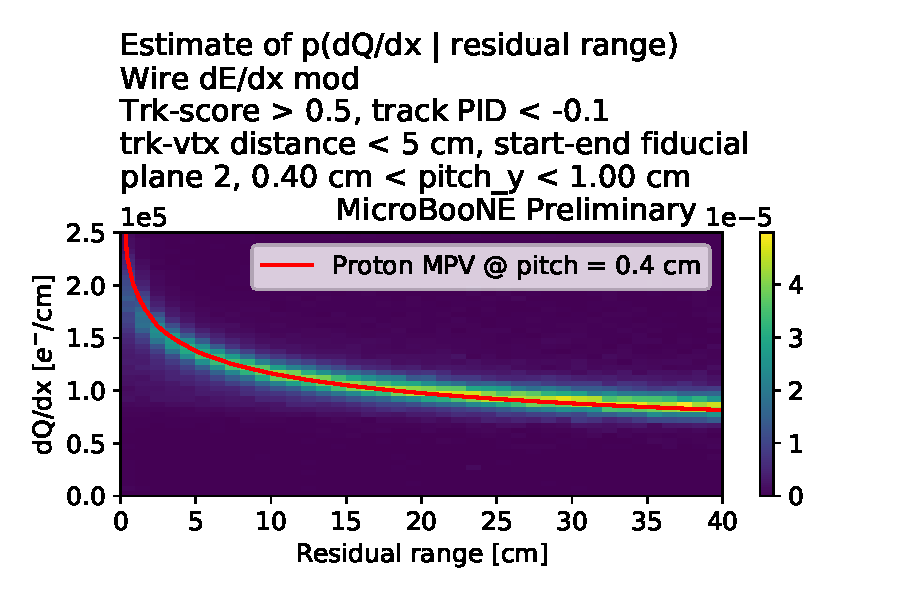
\includegraphics[width=1.00\textwidth]{detsys/calorimetry_dqdx/bnb_nu_wire_dedx_mod_04_pitch_y_10.pdf}
    \caption{\label{fig:syst:dedx_vs_rr:wire_mod} WireMod \dedx sample.}
    \end{subfigure}
\caption{\label{fig:syst:dedx_vs_rr}2-dimensional histogram of \dqdx and residual range for the same contained proton selection in data, simulation central value, and WireMod \dedx sample, respectively.
Only hits with pitch between 0.4 cm and 1 cm are used for this comparison, and every vertical slice is normalised to one in order to reduce the dependence of these comparisons on the track kinematics.
The red theoretical curves are helpful in guiding the eye in the comparisons between the data and the two simulations.}
\end{center}
\end{figure}

\subsubsection{Impact of sample statistics on detector systematics evaluation}
\par Limited sample statistics make it difficult to estimate detector systematics with the full selections. This is particularly true for the \zpsel and for the assessment of detector systematics on backgrounds for which sample statistics are particularly low. The impact that sample statistics have on assessing accurate detector systematics is illustrated by figure~\ref{fig:detsysstatlimitation} where, for a fixed bin and fixed selection cuts, the detector systematic uncertainty is estimated with progressively a larger fraction of total available MC events. On the image on the left the computed fractional uncertainty is shown as a function of sample statistics used. The spread in results becomes increasingly large as the sample statistics decrease. In the image on the right the mean uncertainty obtained by averaging results from each of the sub-samples in a vertical band are highlighted. While the mean computed uncertainty shows a stable behavior for any choice of sample statistics (roughly a 2\% uncertainty), when the spread in results is larger than the magnitude of the underlying detector uncertainty, the method used to assess detector systematics tends to significantly over-estimate the systematic uncertainty. 

\begin{figure}[ht] 
\begin{center}
    \begin{subfigure}[b]{0.35\textwidth}
    \centering
    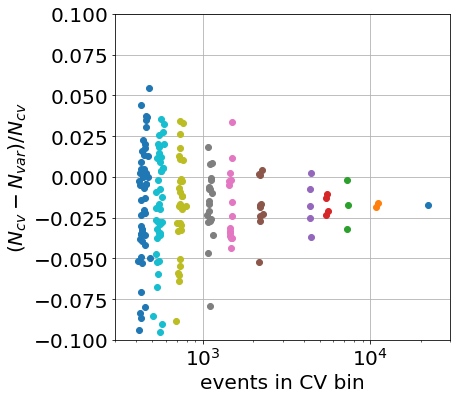
\includegraphics[width=1.00\textwidth]{detsys/detsysstats00.png}
    \caption{Box Cut selection}
    \end{subfigure}
    \begin{subfigure}[b]{0.35\textwidth}
    \centering
    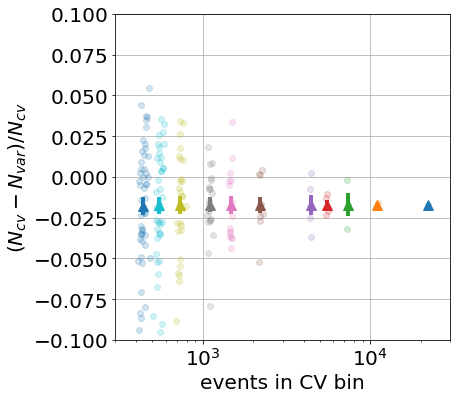
\includegraphics[width=1.00\textwidth]{detsys/detsysstats01.png}
    \caption{BDT selection}
    \end{subfigure}
\caption{\label{fig:detsysstatlimitation} Impact of sample statistics on the evaluation of detector systematic uncertainties. Further details in the text.}
\end{center}
\end{figure}
\par This observation leads to the following practical consequences for the analysis:
\begin{enumerate}
    \item For $\nu_e$ events the full Run1-2-3 $\nu_e$ intrinsic and Run1-3 eLEE low (0-400 MeV) and high (400-800) MeV samples are used to obtain as high statistics as possible over the entire $\nu_e$ energy spectrum.
    \item Detector systematics are evaluated using bins that have at least $\mathcal{O}$(100) raw events in orer to not be sensitive to statistical fluctuations that are too large. For the \npsel we are able to maintain 100 MeV bins while satisfying this requirement, while for the \zpsel we choose 200 MeV bins up to 1.05 GeV in reconstructed energy, and compute detector systematic uncertainties for events in the 1.05-2.05 GeV range in a single bin.
    \item Sample statistics for \numu CC and NC backgrounds to the exclusive \nue selections are too low once final selection cuts are applied, making it impossible to assess detector systematics on these events. Currently a flat 20\% detector systematic is assigned to these background events. Because of the high purity of the analysis, backgrounds are subject to $\mathcal{O}$(100\%) statistical fluctuations making detector uncertainties negligible in comparison.
\end{enumerate}

\subsubsection{Detector systematics on the \npsel, \zpsel, and \numu selections}
\label{sec:detsys:selections}

\par Detector systematics are evaluated by applying the full event selections on identically overlapping sets of events simulated with the CV simulation and the various detector-variation simulations. The event count in each bin under these different variations is evaluated, as shown in figure~\ref{fig:detsys:selection}. Bin to bin variations are then used to construct a covariance matrix (right in figure~\ref{fig:detsys:selection}). The square root of diagonal entries (displayed with their numerical value in the matrix) are then taken as the systematic uncertainty associated to any given variation. Off-diagonal correlations in detector variations are not utilized in this analysis, in part due to the limitation of the uni-sim approach. The impact of different detector variations is finally added in quadrature for all variations to assess the final detector systematic uncertainty for each bin for each selection. The result for the \npsel, \zpsel BDT-based, and \numu selections are shown in tables~\ref{tab:detsys:nue:np:BDT},~\ref{tab:detsys:nue:zp:BDT},  and~\ref{tab:detsys:numu} respectively. Systematics are of order 10-20\% depending on the bin. %Figures showing the bin-to-bin systematic uncertainty for various selections, and at different stages in the selections, are in appendix~\ref{app:detsys:selections}.
FIgure~\ref{fig:detsys:numu} shows the final event kinematics distributions with all systematics, including detector uncertainties, for selected \numu events used in the \numu constraint.



\begin{figure}[H]
    \centering
    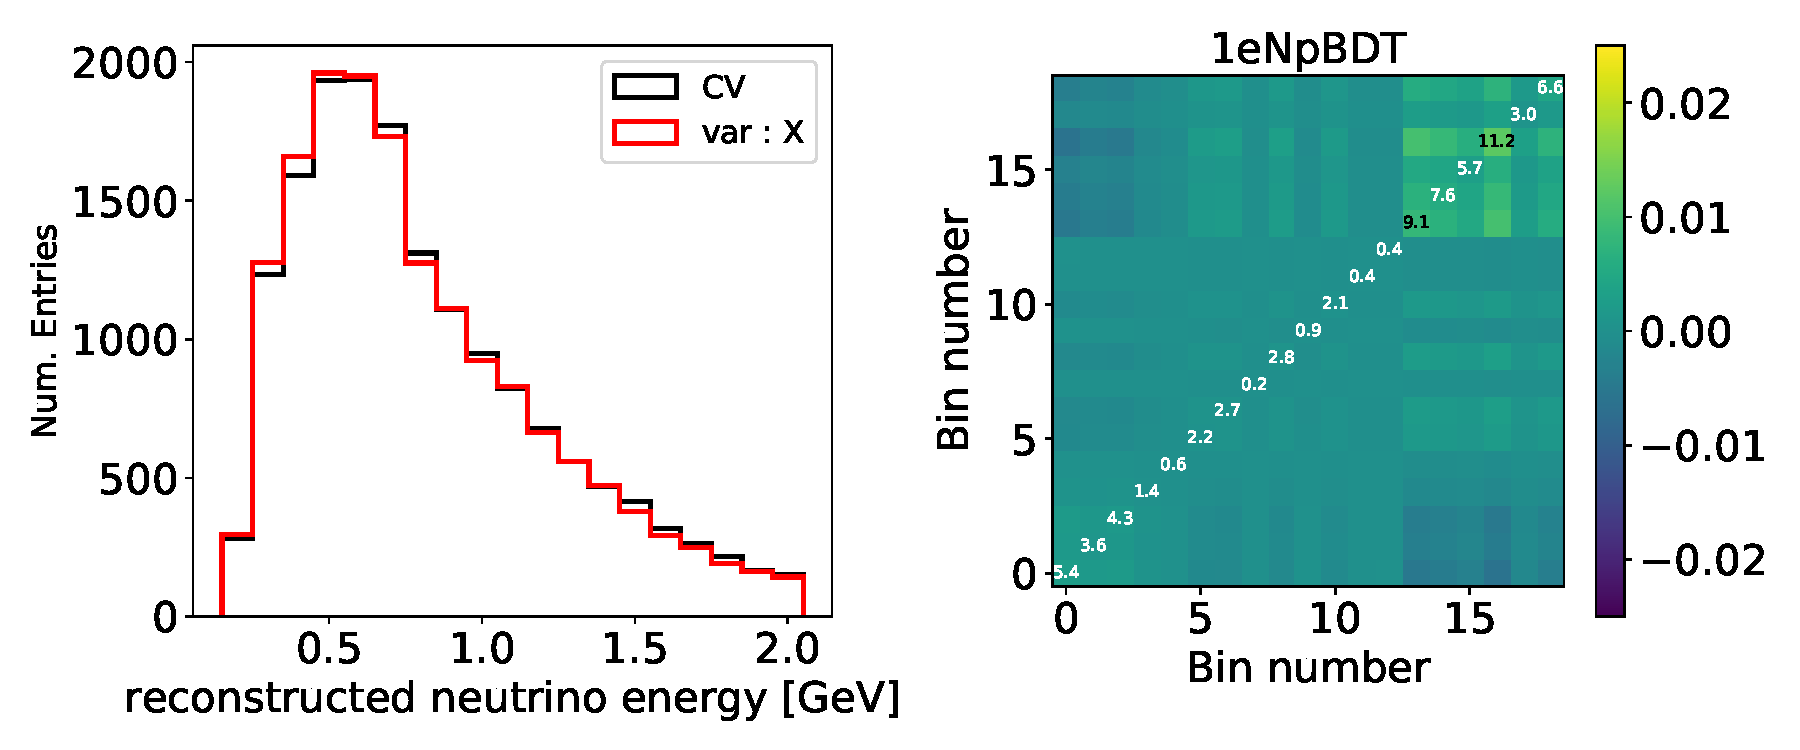
\includegraphics[width=0.7\textwidth]{detsys/reco_e_07252020_1eNpBDT_X.pdf}
\caption{\label{fig:detsys:selection}Example of the impact of the \texttt{WireMod X} variation on the \npsel BDT selection. Left: comparison of selected events in the CV (black) vs. variation (red). The y-scale shows the raw event statistics in the samples, without POT scaling. Right: covariance matrix for this variation with diaognal entries marked by the square-root of the covariance, representative of each bin's percent uncertainty. Sample statistics impact significantly the ability to compute detector systematic uncertainties, with bins with less than a few hundred entries leading to large statistical fluctuations as can be seen in the upper right quadrant of the covariance matrix.}
\end{figure}


\par Tables~\ref{tab:detsys:nue:np:BDT} and~\ref{tab:detsys:nue:zp:BDT} shows the magnitude of detector systematic effects on the and BDT-based \npsel and \zpsel selections. %The impact on the box-cut selection, with very similar results, is available in appendix.~\ref{app:detsys} in table~\ref{tab:detsys:nue:box}.


\begin{table}[H]
\centering
\small
\setlength{\tabcolsep}{3pt}
\renewcommand{\arraystretch}{1.25}
 \begin{tabular}{| c | c | c | c | c | c | c | c | c | c | c | c |} 
 \hline
E [GeV] & scale X & scale YZ & angle YZ & angle XZ & dEdX & SCE & LY down & Rayleigh & LY Attn. & $\Sigma$ \\ \hline
0.15-0.25 & 0.054 & 0.092 & 0.099 & 0.022 & 0.047 & 0.123 & 0.000 & 0.014 & 0.032 &  0.201 \\
0.25-0.35 & 0.036 & 0.036 & 0.059 & 0.000 & 0.060 & 0.044 & 0.000 & 0.000 & 0.000 &  0.108 \\
0.35-0.45 & 0.042 & 0.000 & 0.014 & 0.000 & 0.042 & 0.069 & 0.000 & 0.000 & 0.000 &  0.092 \\
0.45-0.55 & 0.014 & 0.014 & 0.037 & 0.000 & 0.033 & 0.010 & 0.000 & 0.000 & 0.017 &  0.057 \\
0.55-0.65 & 0.000 & 0.020 & 0.010 & 0.014 & 0.010 & 0.059 & 0.010 & 0.000 & 0.000 &  0.066 \\
0.65-0.75 & 0.022 & 0.000 & 0.014 & 0.014 & 0.036 & 0.058 & 0.000 & 0.000 & 0.010 &  0.075 \\
0.75-0.85 & 0.028 & 0.000 & 0.030 & 0.000 & 0.014 & 0.053 & 0.000 & 0.000 & 0.022 &  0.072 \\
0.85-0.95 & 0.000 & 0.042 & 0.010 & 0.010 & 0.028 & 0.062 & 0.020 & 0.000 & 0.022 &  0.087 \\
0.95-1.05 & 0.028 & 0.022 & 0.073 & 0.010 & 0.017 & 0.044 & 0.010 & 0.000 & 0.020 &  0.097 \\
1.05-1.15 & 0.010 & 0.014 & 0.026 & 0.022 & 0.091 & 0.010 & 0.000 & 0.000 & 0.028 &  0.103 \\
1.15-1.25 & 0.020 & 0.010 & 0.096 & 0.040 & 0.032 & 0.227 & 0.000 & 0.000 & 0.032 &  0.255 \\
1.25-1.35 & 0.000 & 0.039 & 0.036 & 0.051 & 0.037 & 0.000 & 0.000 & 0.000 & 0.020 &  0.085 \\
1.35-1.45 & 0.000 & 0.065 & 0.108 & 0.020 & 0.052 & 0.032 & 0.000 & 0.010 & 0.017 &  0.143 \\
1.45-1.55 & 0.091 & 0.000 & 0.041 & 0.039 & 0.122 & 0.060 & 0.010 & 0.010 & 0.030 &  0.176 \\
1.55-1.65 & 0.076 & 0.041 & 0.130 & 0.066 & 0.017 & 0.042 & 0.000 & 0.010 & 0.040 &  0.181 \\
1.65-1.75 & 0.057 & 0.058 & 0.000 & 0.033 & 0.000 & 0.173 & 0.010 & 0.000 & 0.063 &  0.204 \\
1.75-1.85 & 0.112 & 0.022 & 0.058 & 0.081 & 0.036 & 0.065 & 0.000 & 0.000 & 0.074 &  0.184 \\
1.85-1.95 & 0.030 & 0.010 & 0.131 & 0.014 & 0.030 & 0.082 & 0.020 & 0.000 & 0.047 &  0.169 \\
1.95-2.05 & 0.066 & 0.053 & 0.024 & 0.067 & 0.053 & 0.125 & 0.010 & 0.000 & 0.046 &  0.181 \\
 \hline
 \end{tabular}
 \caption{\label{tab:detsys:nue:np:BDT} Detector systematics for BDT \npsel selection. The final column is the quadrature sum of all systematic variations.}
\end{table}



\begin{table}[H]
\centering
\small
\setlength{\tabcolsep}{3pt}
\renewcommand{\arraystretch}{1.25}
 \begin{tabular}{| c | c | c | c | c | c | c | c | c | c | c | c |} 
 \hline
E [GeV] & scale X & scale YZ & angle YZ & angle XZ & dEdX & SCE & LY down & Rayleigh & LY Attn. & $\Sigma$ \\ \hline
0.15-0.35 & 0.000 & 0.039 & 0.089 & 0.000 & 0.000 & 0.000 & 0.010 & 0.010 & 0.000 &  0.098 \\
0.35-0.55 & 0.000 & 0.014 & 0.028 & 0.037 & 0.061 & 0.057 & 0.010 & 0.000 & 0.030 &  0.101 \\
0.55-0.75 & 0.030 & 0.000 & 0.022 & 0.020 & 0.000 & 0.185 & 0.010 & 0.017 & 0.026 &  0.193 \\
0.75-0.95 & 0.040 & 0.010 & 0.010 & 0.042 & 0.000 & 0.214 & 0.014 & 0.014 & 0.065 &  0.233 \\
0.95-1.15 & 0.042 & 0.053 & 0.057 & 0.071 & 0.052 & 0.302 & 0.010 & 0.022 & 0.024 &  0.329 \\
1.15-2.15 & 0.037 & 0.014 & 0.010 & 0.066 & 0.045 & 0.143 & 0.017 & 0.014 & 0.024 & 0.172 \\
 \hline
 \end{tabular}
 \caption{\label{tab:detsys:nue:zp:BDT} Detector systematics for BDT \zpsel selection. The final column is the quadrature sum of all systematic variations.}
\end{table}



\par The impact of detector systematics on the $\nu_{\mu}$ selection can be found in table~\ref{tab:detsys:numu}. Figure~\ref{fig:detsys:numu} shows the primary kinematics distributions for the $\nu_{\mu}$ selection, including detector systematics.

\begin{table}[H]
\centering
\small
\setlength{\tabcolsep}{3pt}
\renewcommand{\arraystretch}{1.25}
 \begin{tabular}{| c | c | c | c | c | c | c | c | c | c | c | c | c | c | } 
 \hline
    E [GeV] & LY attn & LY Down & Rayleigh & SCE & X & YZ & Angle XZ & Angle YZ & dEdX & Recomb & $\Sigma$ \\ \hline
0.15-0.25 & 0.034 & 0.006 & 0.018 & 0.027 & 0.049 & 0.003 & 0.043 & 0.031 & 0.041 & 0.064 & 0.096 \\
0.25-0.35 & 0.026 & 0.004 & 0.0 & 0.045 & 0.035 & 0.061 & 0.04 & 0.009 & 0.012 & 0.016 & 0.097 \\
0.35-0.45 & 0.001 & 0.009 & 0.009 & 0.039 & 0.02 & 0.016 & 0.042 & 0.013 & 0.011 & 0.042 & 0.066 \\
0.45-0.55 & 0.006 & 0.003 & 0.003 & 0.015 & 0.017 & 0.002 & 0.003 & 0.005 & 0.045 & 0.03 & 0.051 \\
0.55-0.65 & 0.014 & 0.005 & 0.009 & 0.002 & 0.009 & 0.045 & 0.018 & 0.02 & 0.032 & 0.014 & 0.065 \\
0.65-0.75 & 0.008 & 0.008 & 0.006 & 0.017 & 0.024 & 0.033 & 0.051 & 0.022 & 0.059 & 0.118 & 0.093 \\
0.75-0.85 & 0.025 & 0.005 & 0.002 & 0.044 & 0.0 & 0.045 & 0.012 & 0.008 & 0.041 & 0.003 & 0.081 \\
0.85-0.95 & 0.009 & 0.013 & 0.006 & 0.01 & 0.016 & 0.016 & 0.016 & 0.031 & 0.053 & 0.012 & 0.07 \\
0.95-1.05 & 0.034 & 0.017 & 0.008 & 0.023 & 0.008 & 0.067 & 0.072 & 0.013 & 0.005 & 0.043 & 0.109 \\
1.05-1.15 & 0.031 & 0.019 & 0.006 & 0.034 & 0.064 & 0.025 & 0.062 & 0.006 & 0.062 & 0.015 & 0.122 \\
1.15-1.25 & 0.05 & 0.025 & 0.0 & 0.053 & 0.075 & 0.017 & 0.058 & 0.008 & 0.07 & 0.05 & 0.142 \\
1.25-1.35 & 0.031 & 0.03 & 0.015 & 0.119 & 0.015 & 0.031 & 0.061 & 0.046 & 0.043 & 0.019 & 0.158 \\
1.35-1.45 & 0.0 & 0.022 & 0.0 & 0.048 & 0.064 & 0.085 & 0.021 & 0.064 & 0.118 & 0.059 & 0.18 \\
1.45-1.55 & 0.054 & 0.028 & 0.054 & 0.03 & 0.162 & 0.054 & 0.135 & 0.081 & 0.08 & 0.1 & 0.261 \\
 \hline
 \end{tabular}
 \caption{\label{tab:detsys:numu} Detector systematics for $\nu_{\mu}$ selection.}
\end{table}

\begin{figure}[H] 
\begin{center}
    \begin{subfigure}[b]{0.3\textwidth}
    \centering
    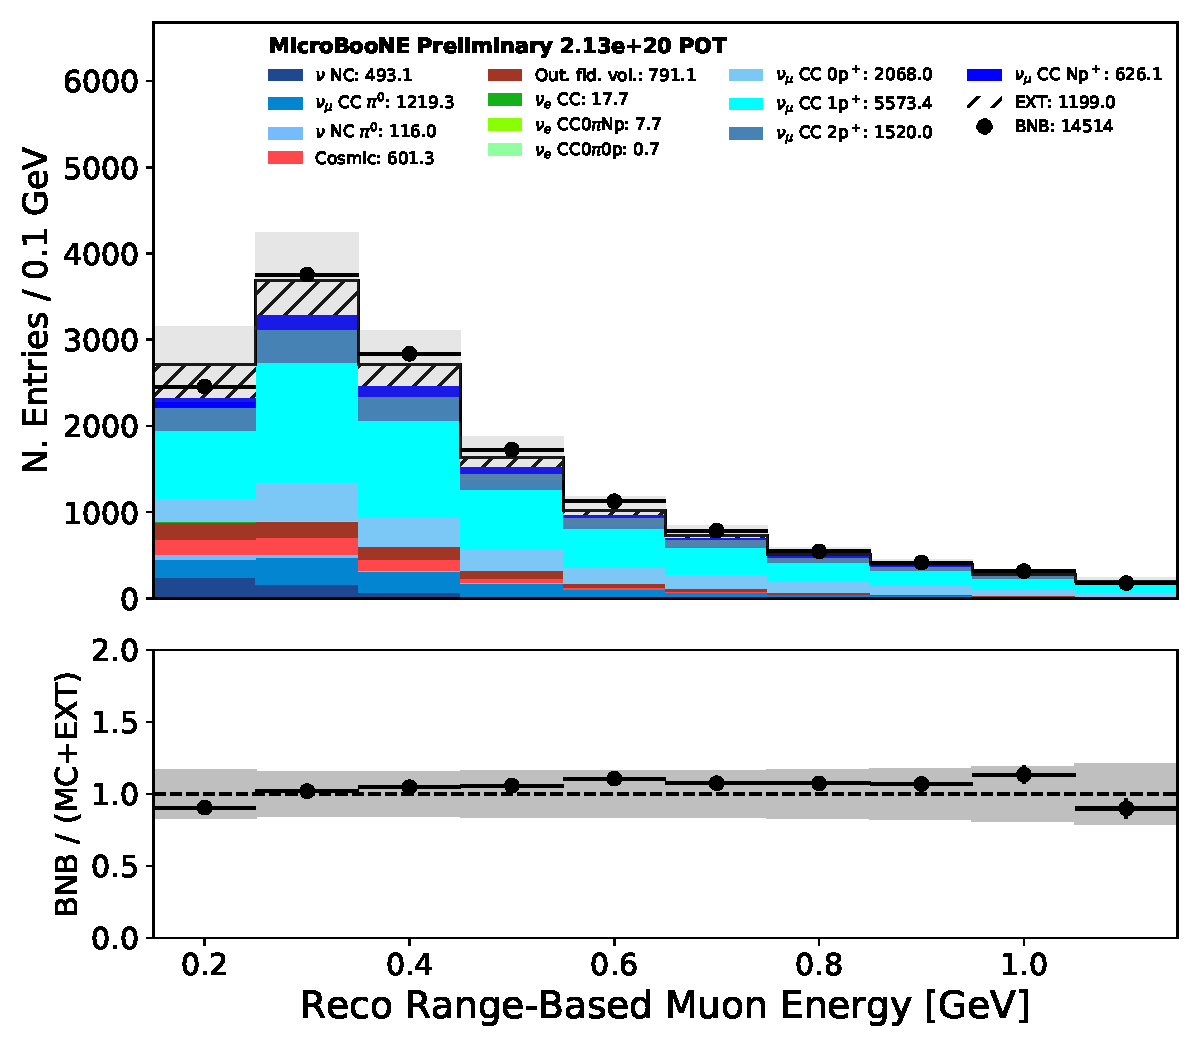
\includegraphics[width=1.00\textwidth]{NuMuCCsel/Images/Ryan/fullselection_run3_fullsystematics/trk_range_muon_e_v_07232020_fullsel_samples_detsys_event_category.pdf}
    \caption{\label{fig:detsys:numu:muonrange} muon range KE}
    \end{subfigure}
        \begin{subfigure}[b]{0.3\textwidth}
    \centering
    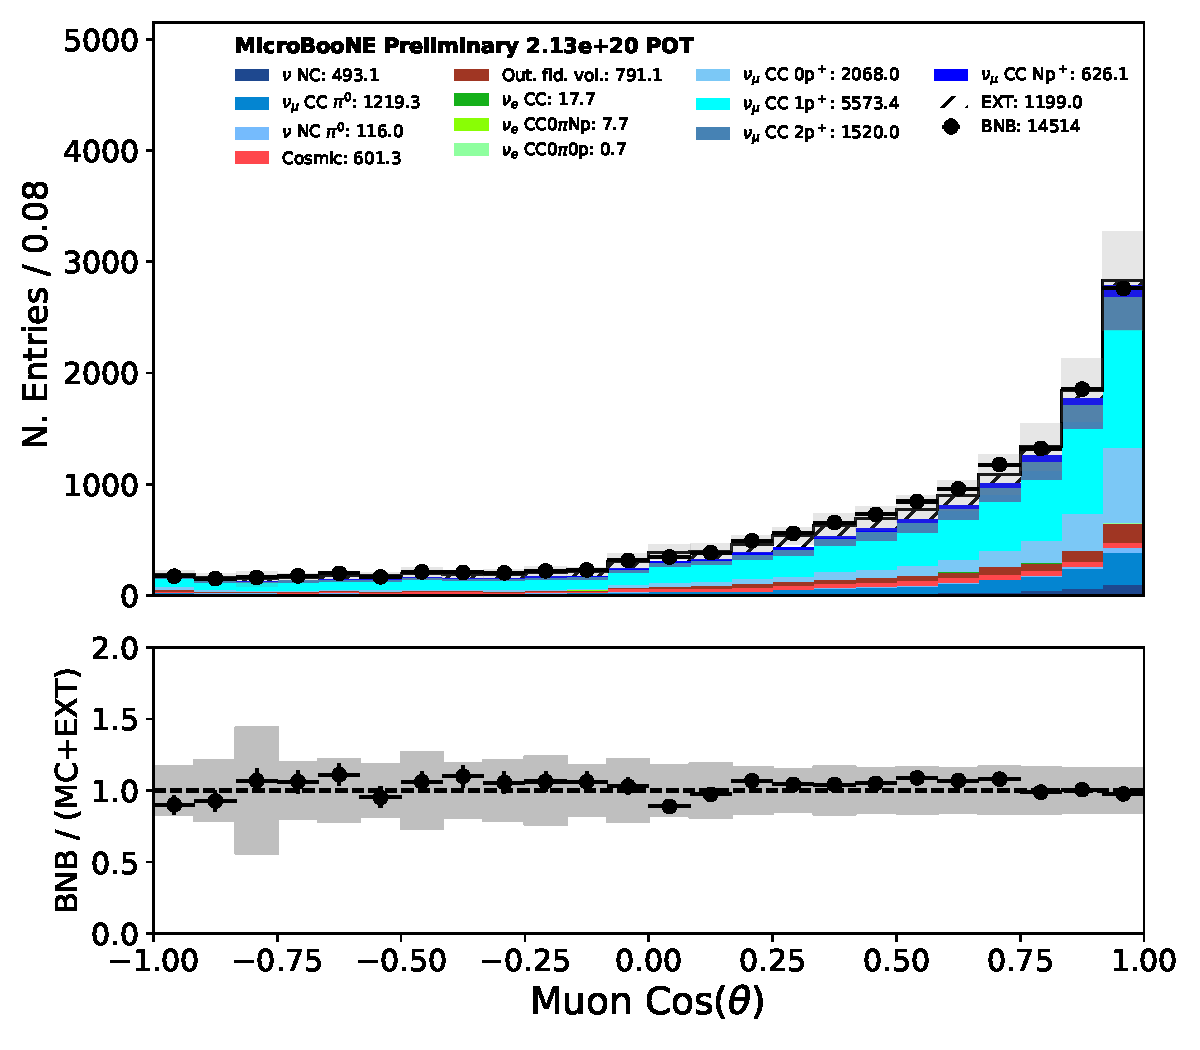
\includegraphics[width=1.00\textwidth]{NuMuCCsel/Images/Ryan/fullselection_run3_fullsystematics/trk_cos_theta_v_07232020_fullsel_samples_detsys_event_category.pdf}
    \caption{\label{fig:detsys:numu:muontheta} muon cos$(\theta)$}
    \end{subfigure}
        \begin{subfigure}[b]{0.3\textwidth}
    \centering
    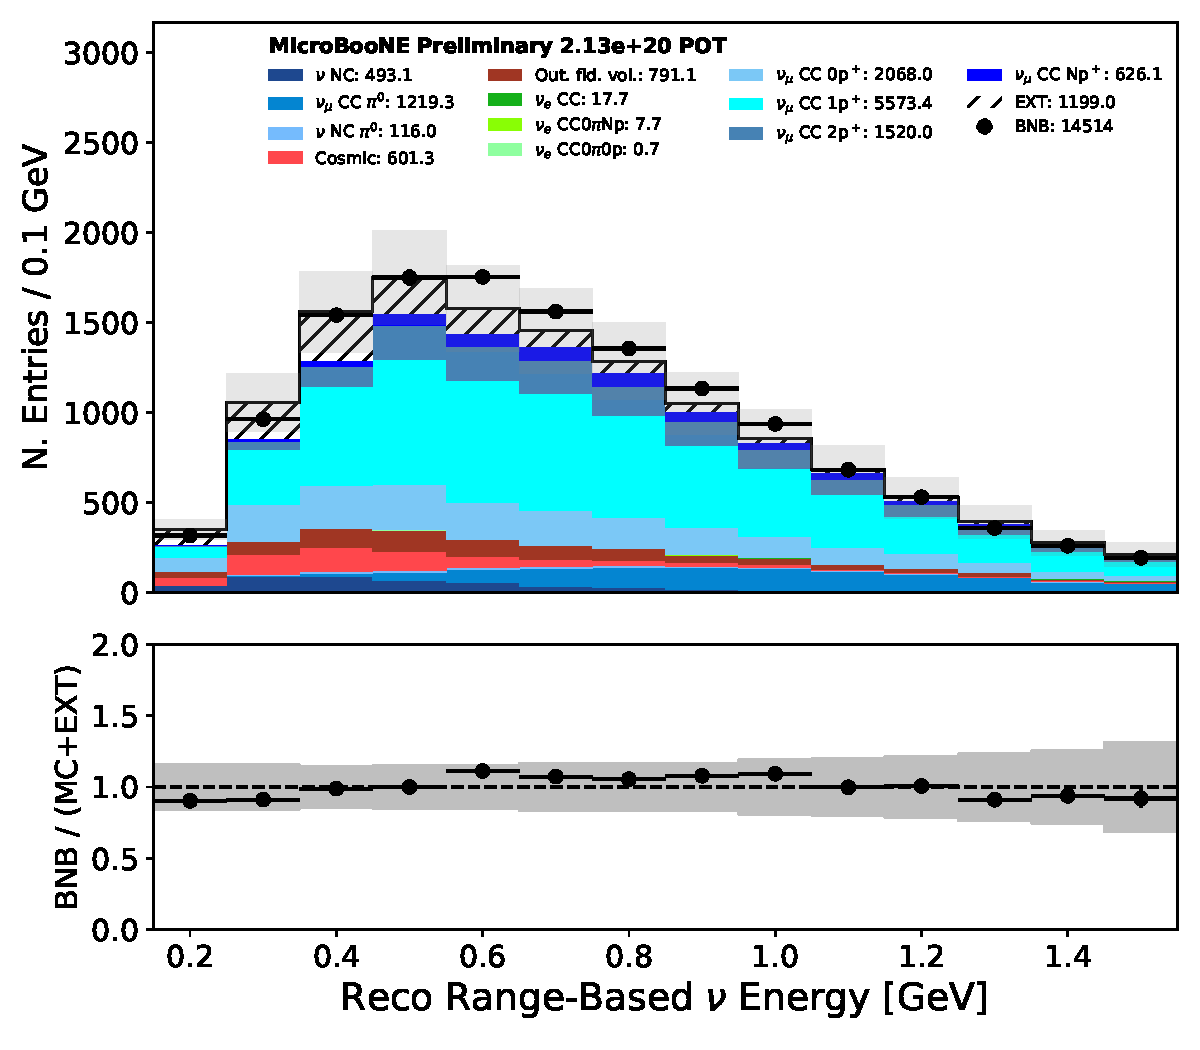
\includegraphics[width=1.00\textwidth]{NuMuCCsel/Images/Ryan/fullselection_run3_fullsystematics/reco_nu_e_range_v_07232020_fullsel_samples_detsys_event_category.pdf}
    \caption{\label{fig:detsys:numu:nurange} range-based $\nu$ energy}
    \end{subfigure}
\caption{\label{fig:detsys:numu}Run3 $2.13E20$ POT $\nu_{\mu}$ distributions with detector systematics.}
\end{center}
\end{figure}


\subsection{Flux Uncertainties }
\label{sec:systematics:flux}
%
%The flux \textcolor{blue}{model} and \textcolor{blue}{its} uncertainties for MCC9~\cite{bib:fluxmcc9,bib:fluxtechnote} are largely the same as MCC8~\cite{bib:fluxtechnote}. We use the multisim technique to estimate the flux uncertainties. The various sources of uncertainties are taken as independent and are varied individually around the central value. They are listed in Table~\ref{tab:fluxsyst} along the number of universes considered for each. The fractional covariance matrix and correlation matrix for the 1eNp selection are presented in Figure~\ref{fig:fluxmatrices} which amount to 2\% in flux uncertainties. Meanwhile, Figure~\ref{fig:fluxsystvars} displays the effects of reweighting central value in each universe of an individual parameter of flux.

The flux model and its uncertainties for MCC9~\cite{bib:fluxmcc9,bib:fluxtechnote} are largely the same as MCC8~\cite{bib:fluxtechnote} and originate from the implementation performed in MiniBooNE~\cite{bib:MBflux}. We use the many universes method to estimate the flux uncertainties. The various sources of uncertainties are taken as independent and  are individually varied by drawing from a Gaussian of width $\pm 1 \sigma$ of their measured uncertainties. The excursion of the variations from each such draw is commonly referred to as a universe. The sources of uncertainty considered are listed in Table~\ref{tab:fluxsyst}. In this analysis, the 13 flux parameter variations are varied simultaneously according to a Gaussian distribution for 1000 universes.
Figure~\ref{fig:fluxsystvars} displays the effects of reweighting central value in each universe for individual parameters of the flux model. The systematic error is calculated from the difference of the expected events in the various universes with respect to the central value. Therefore the width of the variations in the plots represents the size of systematic uncertainty expected for each individual parameter of the flux model.
The fractional covariance matrix for the \npsel and \zpsel selections are presented in Figure~\ref{fig:fluxmatrices} and show about 17\% uncertainty in the lowest visible energy bin (0.15 - 0.25 GeV) for the \npsel selection and 7\% for the \zpsel selection. %@cThe flux systematics are calculated only for the background-only hypothesis, where we do not assign any uncertainties to the LEE signal model. 

\begin{table}[H]
\centering
 \begin{tabular}{| c | m{6cm} | c |} 
    \hline
\hline
Parameter Name & Description & Universes \\
\hline
expskin\_FluxUnisim         &  skin-depth electric currents penetrate conductor & --\\ 
horncurrent\_FluxUnisim           &  horn current in magnetic focusing horns & --\\ 
kminus\_PrimaryHadronNormalization        &  Primary hadron normalization & --\\ 
kplus\_PrimaryHadronFeynmanScaling       & Primary Hadron Feynman Scaling & --\\ 
kzero\_PrimaryHadronSanfordWang        &  Primary Hadron Sanford Wang & --\\ 
nucleoninexsec\_FluxUnisim       &  nucleon total inelastic cross section on Be & --\\  
nucleonqexsec\_FluxUnisim      &  nucleon total quasi-elastic cross section on Be & --\\ 
nucleontotxsec\_FluxUnisim   &  nucleon total cross section on Be & --\\ 
piminus\_PrimaryHadronSWCentralSplineVariation      &  Primary Hadron Sanford Wang Central Spline Variation & --\\ 
pioninexsec\_FluxUnisim   &  pion total inelastic cross section on Be & --\\ 
pionqexsec\_FluxUnisim     &  pion total quasi-elastic cross section on Be & --\\ 
piontotxsec\_FluxUnisim       &  pion total cross section on Be & --\\ 
piplus\_PrimaryHadronSWCentralSplineVariation     &  Primary Hadron Sanford Wang Central Spline Variation & --\\
\hline
flux\_all               &       13 flux parameters varied randomly and simultaneously according to Gaussian distributions, with 1$\sigma$ uncertainties     & 1000 \\
\hline
\end{tabular}
\caption{List of flux systematic variations used in the Pandora eLEE analysis}
\label{tab:fluxsyst}
\end{table}

\begin{figure}[ht] 
\begin{center}
    \begin{subfigure}[b]{0.48\textwidth}
    \centering
    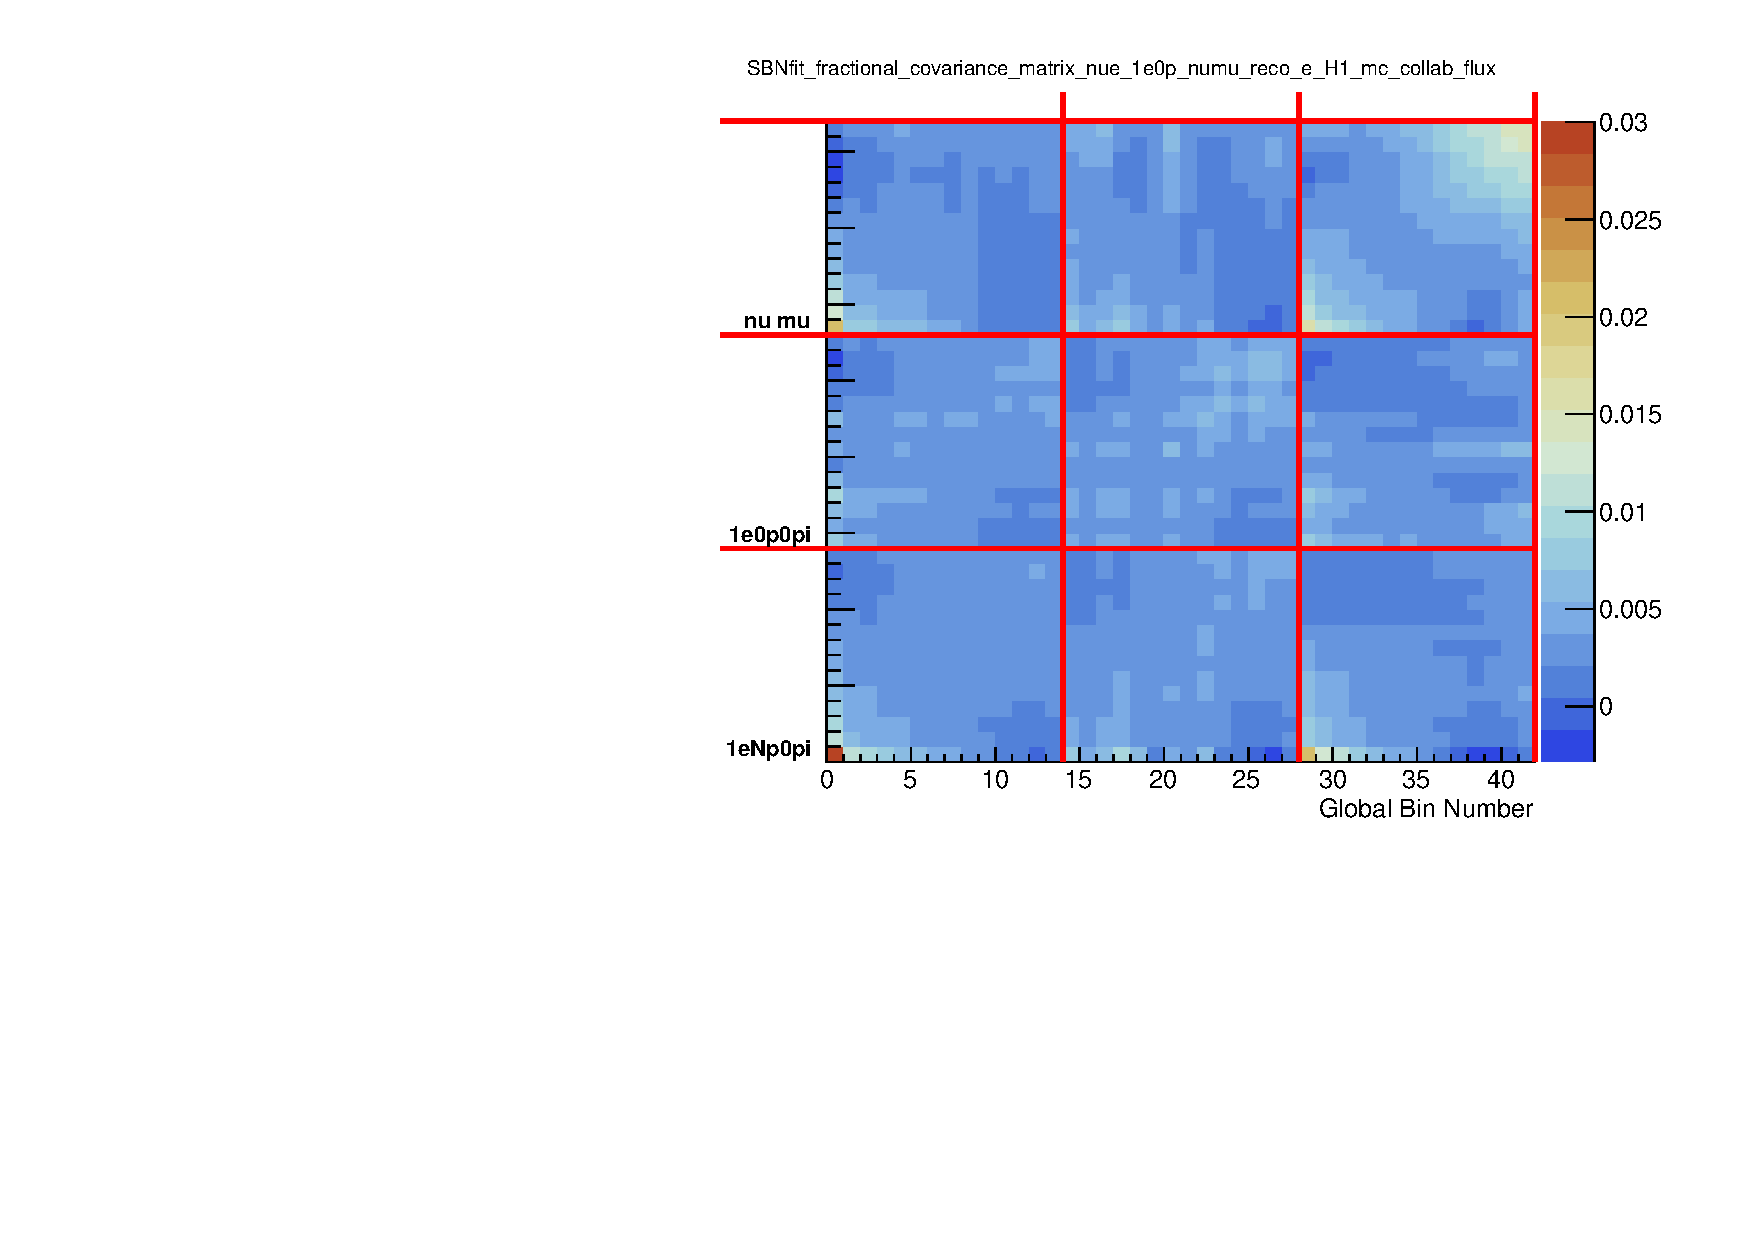
\includegraphics[width=1.00\textwidth]{Systematics/CovarianceMatrices/SBNfit_fractional_covariance_matrix_nue_1e0p_numu_reco_e_H1_mc_collab_flux_collapsed.pdf}
    \caption{flux uncertainty fractional covariance matrix}
    \end{subfigure}
    \begin{subfigure}[b]{0.48\textwidth}
    \centering
    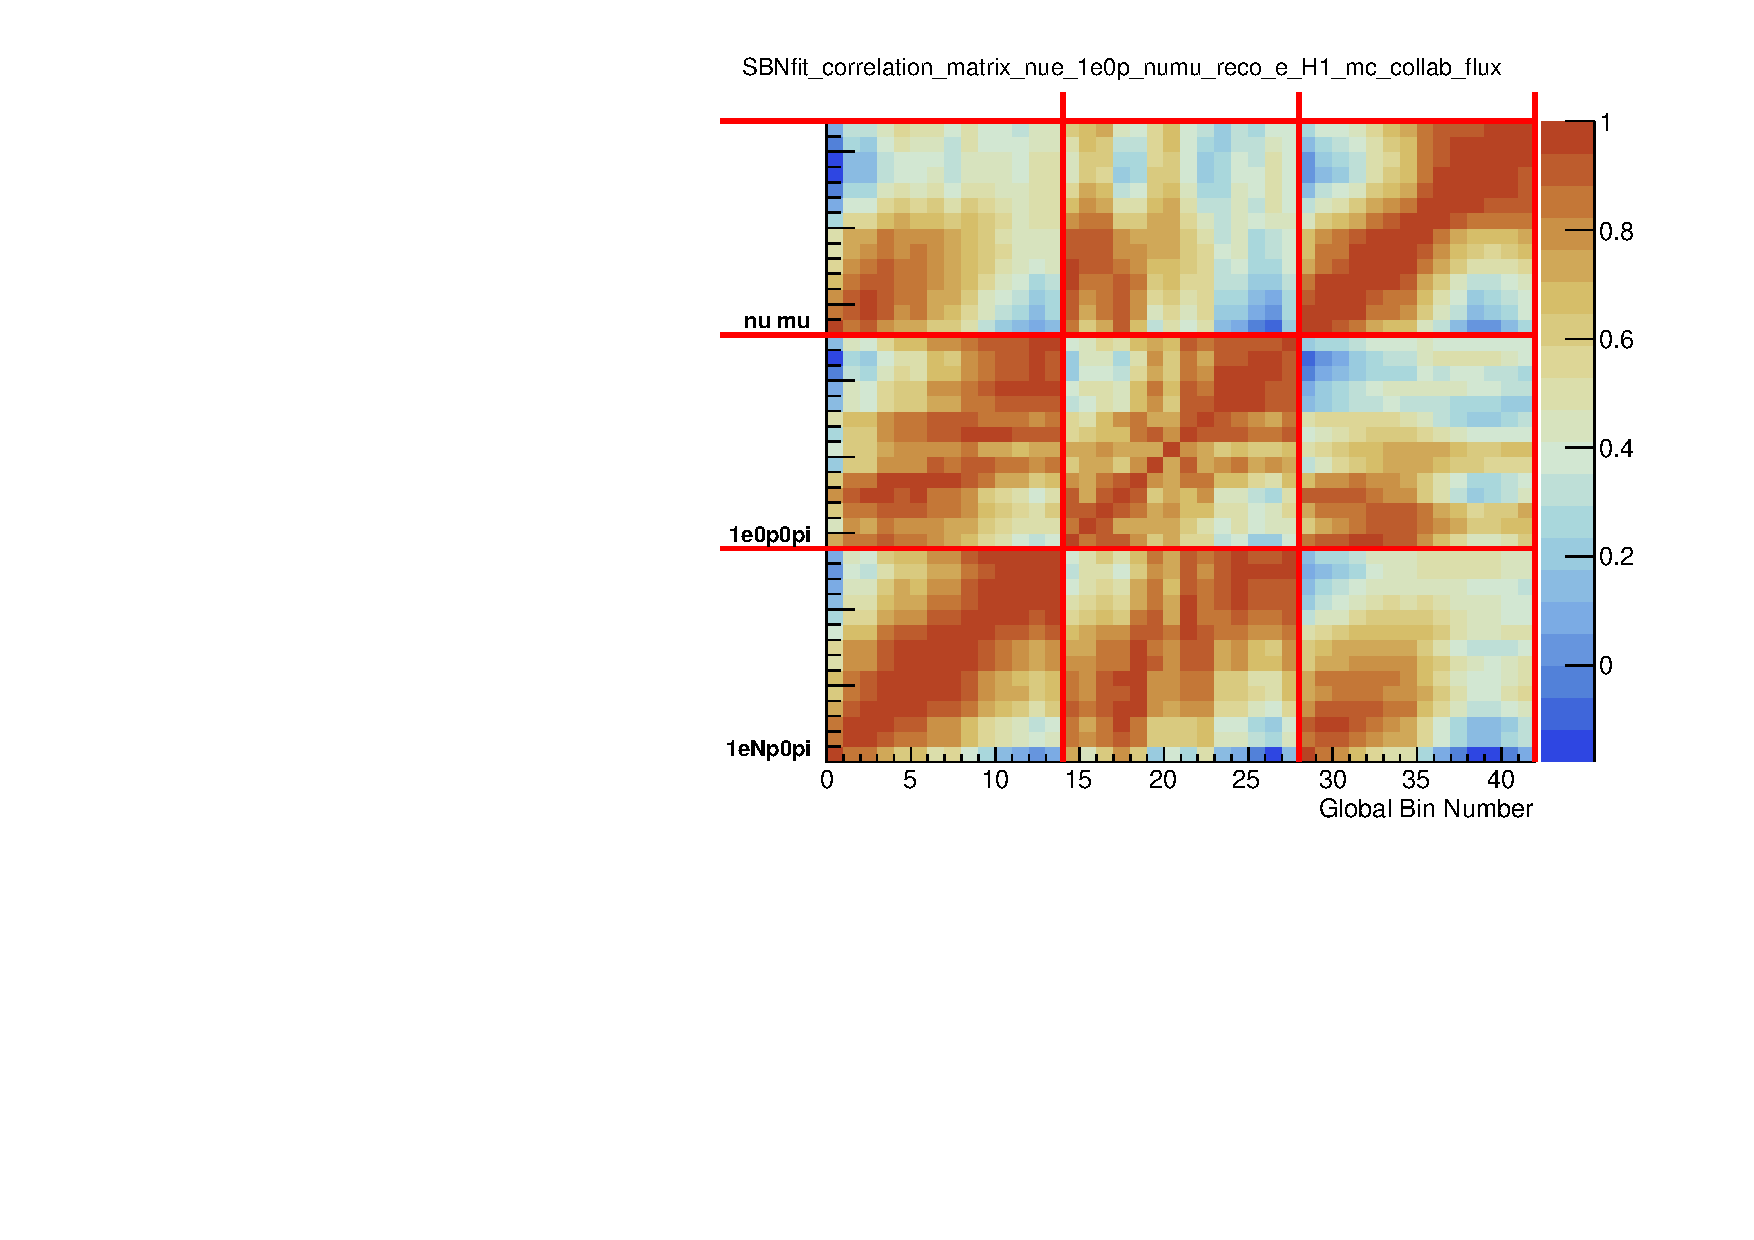
\includegraphics[width=1.00\textwidth]{Systematics/CovarianceMatrices/SBNfit_correlation_matrix_nue_1e0p_numu_reco_e_H1_mc_collab_flux_collapsed.pdf}
    \caption{flux uncertainty correlation matrix}
    \end{subfigure}
\caption{\label{fig:fluxmatrices} Flux only fractional covariance matrix and correlation matrix for the combined \npsel, \zpsel, and \numu selection as a function of reconstructed neutrino energy. The global bin number starts from 0.15 GeV up to 1.55 GeV, in bins of 0.1 GeV.}
\end{center}
\end{figure}

\begin{figure}[H] 
    \centering
    \begin{subfigure}[b]{0.45\textwidth}
    \centering
    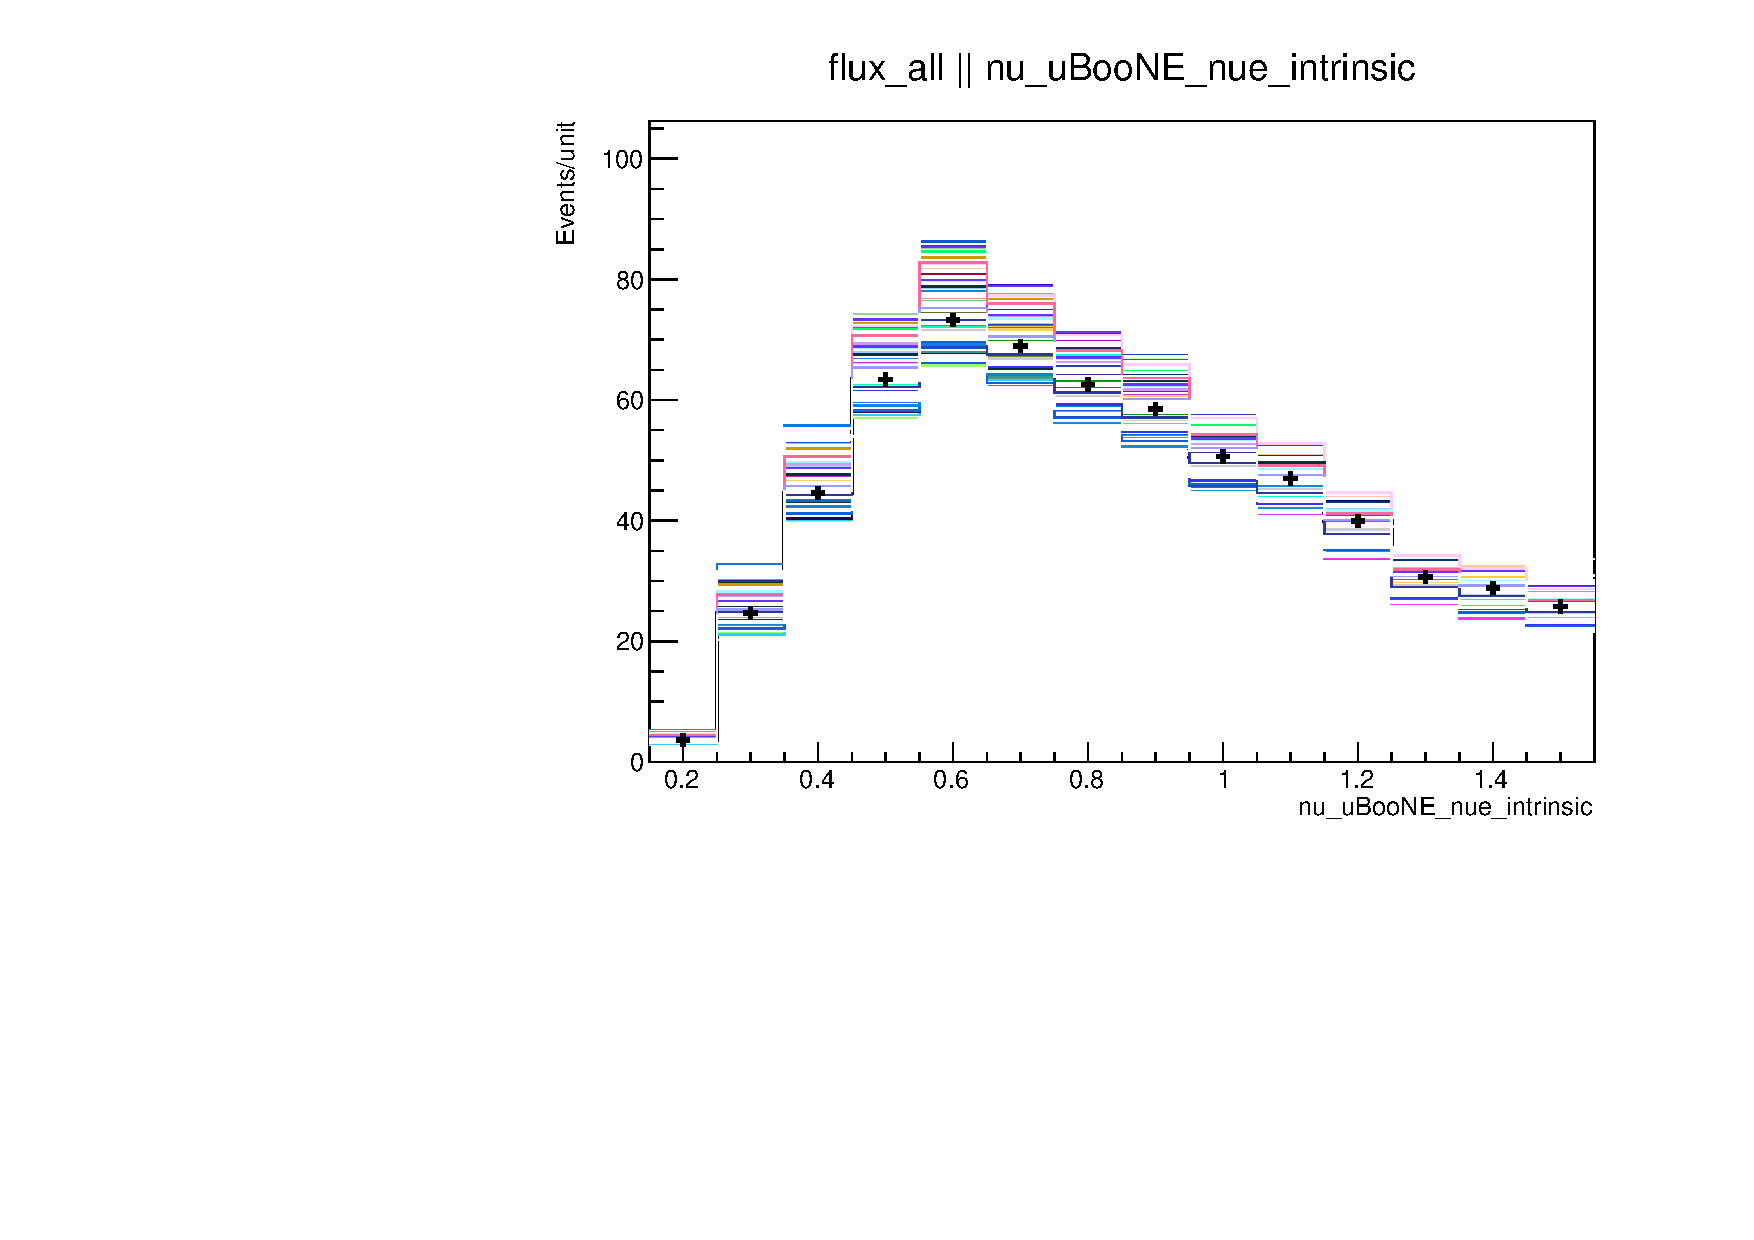
\includegraphics[width=1.00\textwidth]{Systematics/systvariations/BDT/Variation_nue_1e0p_numu_reco_e_H1_mc_collab_flux_all_nu_uBooNE_nue_intrinsic_1D.pdf}
    \caption{\npsel selection}
    \end{subfigure}
    \begin{subfigure}[b]{0.45\textwidth}
    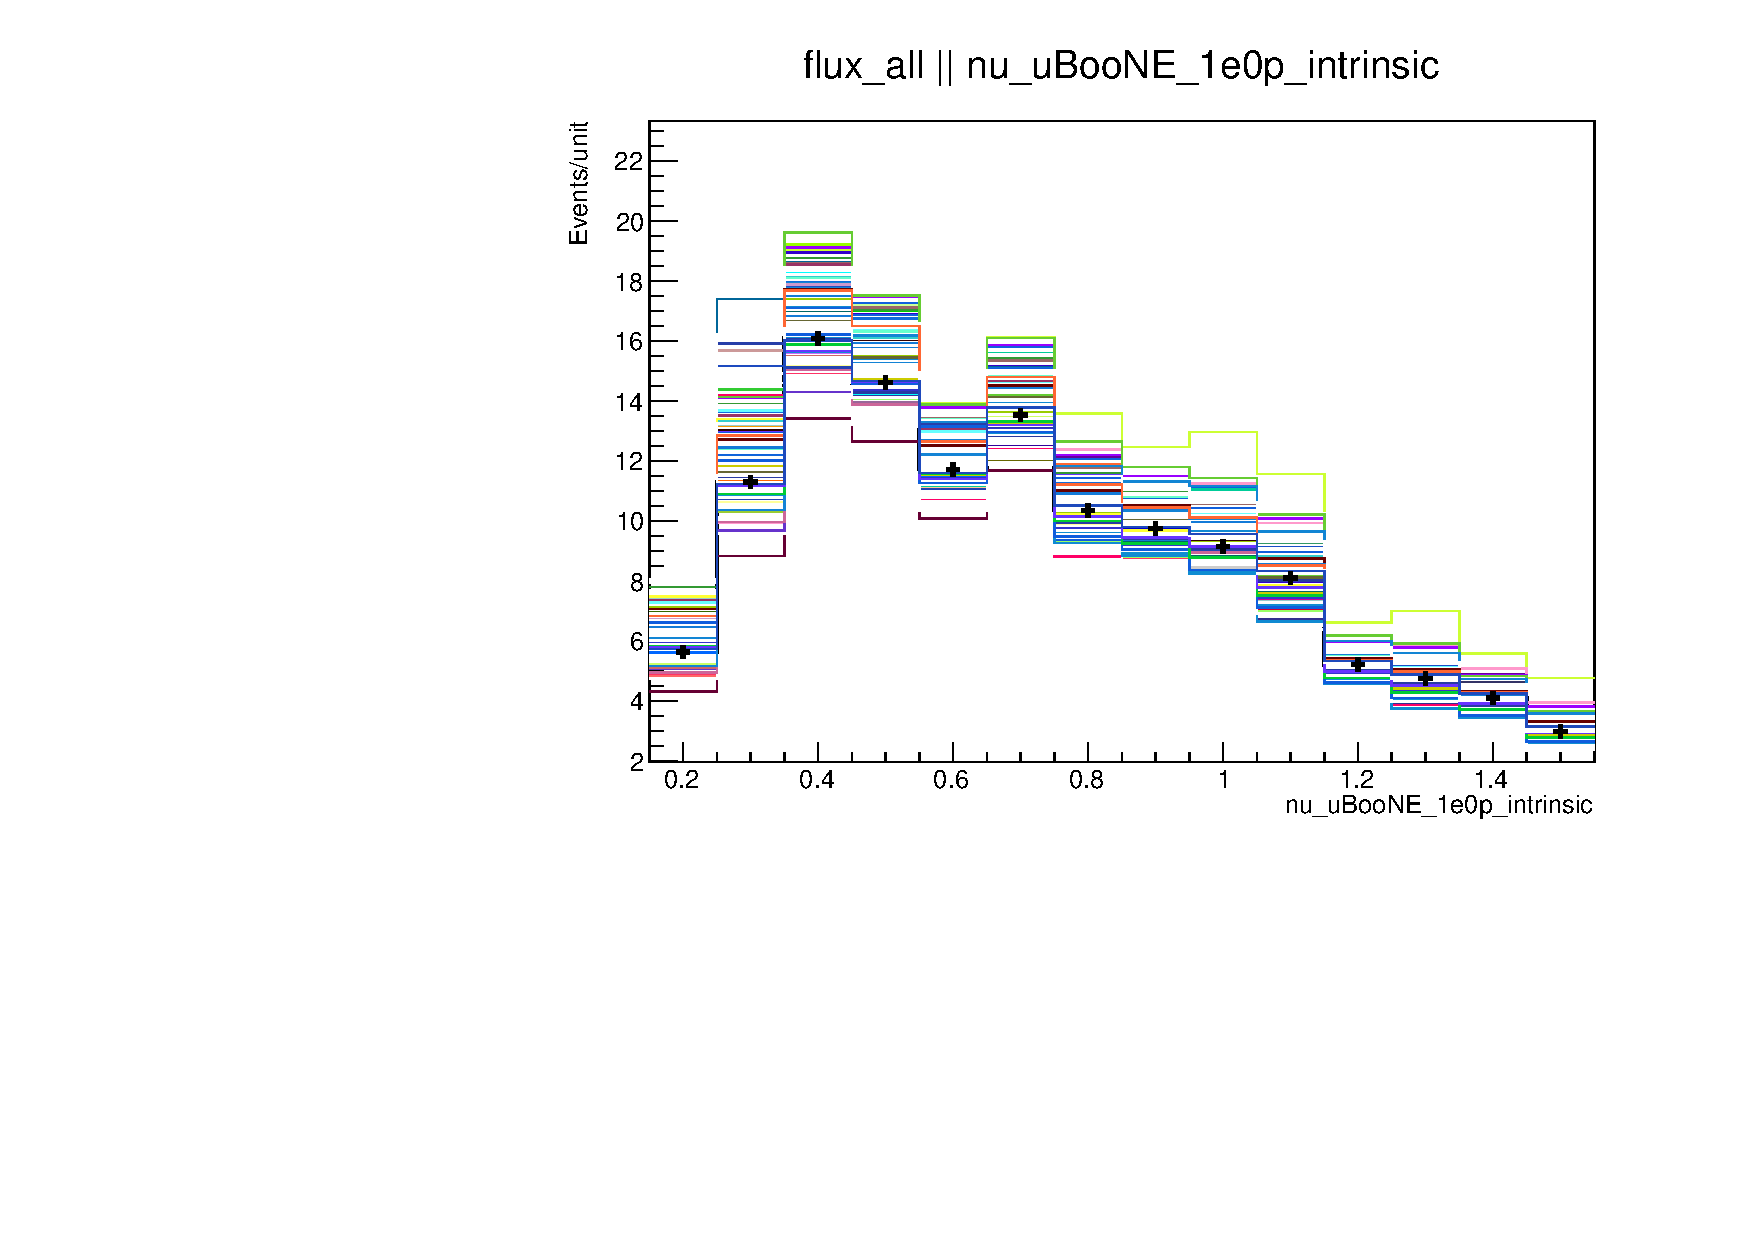
\includegraphics[width=1.00\textwidth]{Systematics/systvariations/BDT/Variation_nue_1e0p_numu_reco_e_H1_mc_collab_flux_all_nu_uBooNE_1e0p_intrinsic_1D.pdf}
    \caption{\zpsel selection}
    \end{subfigure}
\caption{\label{fig:fluxsystvars} The effects of \textit{flux\_all} variations on the intrinsic \nue sub-channel of the \npsel and \zpsel selections. The black crosses show the central value and each multicolored line shows a separate universe's reweighing of the central value. The magnitude of the  uncertainty in each bin corresponds to the average difference between each shifted universe and the central value in that bin.}
\end{figure}

\subsection{Neutrino Interaction Modeling Uncertainties }
\label{sec:systematics:xsec}

We use the \texttt{GENIE} event reweighting framework with the standard reweighting parameters, also known as ``knobs'', to model neutrino cross section and FSI uncertainties. Document~\cite{bib:geniesupportnote} describes the GENIE cross-section model, recommended central-value tune, and the recommended uncertainties for MCC9 analyses. 

The updated Genie central value tune is guided on fits to the T2K data which increase the MA CCQE and scale up the MEC normalization. These provide overall good data-MC agreement in the \numu CC channel as preliminarily shown in sec.~\ref{sec:numuselection}.

A total of 53 sources of uncertainty are considered. The majority of them, 44, are varied with a multisim approach around the updated Genie central value tune. Their variations are simultaneous to take into account their correlations, and are given the name \textit{Genie\_All}. They are listed in Table~\ref{tab:AllGenie}. The variations of the remaining nine sources cover the full range of the parameter values: they are varied from 0 to 1, turning on or off a specific modeling effect. Table~\ref{tab:geniesyst} lists the uncertainties that are used in the analysis and the number of universes investigated. %The genie systematic uncertainty is currently also calculated only for the background-only hypothesis and we do not assign any genie systematics to the unfolded LEE signal model.

The fractional covariance matrix and correlation matrix for the \npsel, \zpsel, and \numu selections are presented in Figure~\ref{fig:geniematrices} which is estimated to be ~20\% in average and up to 50\% at around 0.15 - 0.25 GeV. Meanwhile, Figure~\ref{fig:geniesystvars} displays the effects of reweighting the central value in each universe of an individual genie knob.

One neutrino interaction modeling uncertainty which is still not fully incorporated in the analysis is the uncertainty on the CCMEC interaction kinematics. The current status of the modeling of this knob is presented in \href{https://microboone-docdb.fnal.gov/cgi-bin/private/ShowDocument?docid=31787}{DocDB 31787}. The knob, in a nutshell, allows to reweigh events between the CCMEC ``empirical'' model and the Nieves model (as described in ~\cref{tab:geniesyst}). This knob impacts the kinematics of MEC interactions, but not their rate. In particular, the kinematics of the final state lepton are impacted by the variation. At the time of writing this note, we have been able to assess the preliminary impact of the updated CCMEC knob on the \npsel and \zpsel event rates, but have not folded in this uncertainty in the sensitivity calculation. Figure~\ref{fig:ccmec} shows the impact of the variation on these selections, as well as on the constraint \numu selection. We see that the impact of this knob is at most 10\%, and in the \npsel the variation is smaller at low energies. These comparisons are preliminary as the validation of the knob implementation itself is underway. Motivation for how this variation impacts the selection performance may be attributed to shower energy and shower angle dependency in the final selection efficiencies. Finally, we note the interesting anti-correlation in the impact of this variation between the \npsel and \zpsel selections.

\begin{figure}[H] 
    \begin{center}
    \begin{subfigure}[b]{0.3\textwidth}
    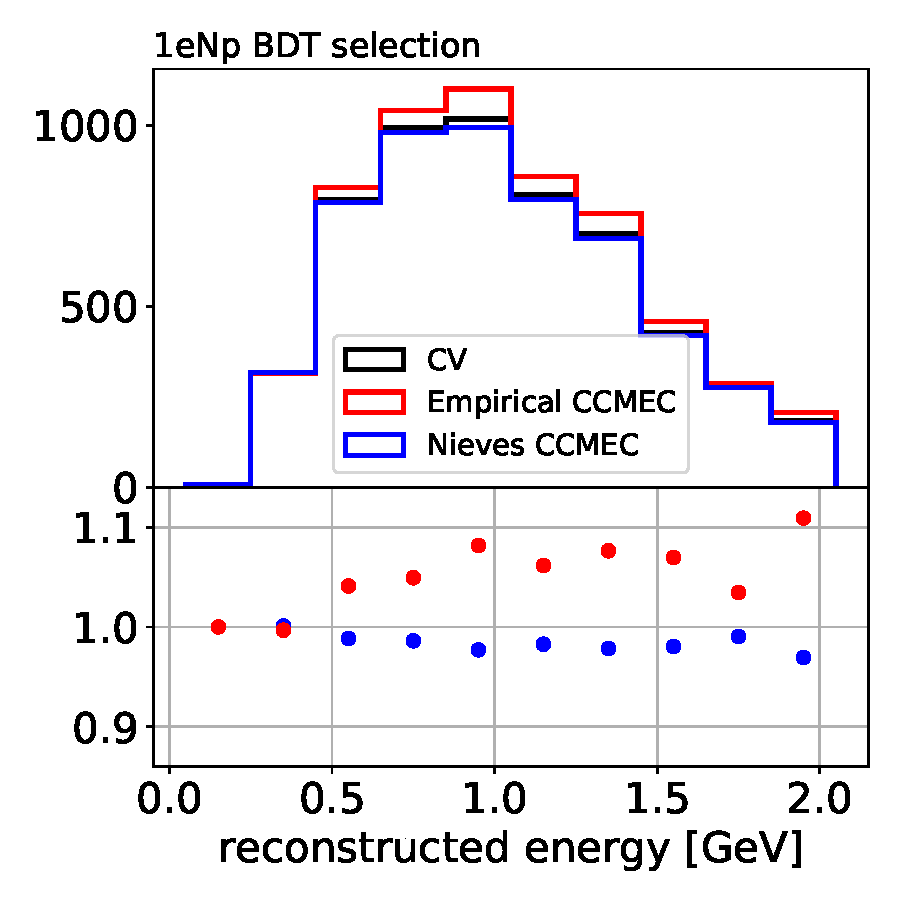
\includegraphics[width=1.00\textwidth]{Systematics/systvariations/1eNp_CCMEC.pdf}
    \end{subfigure}
    \begin{subfigure}[b]{0.3\textwidth}
    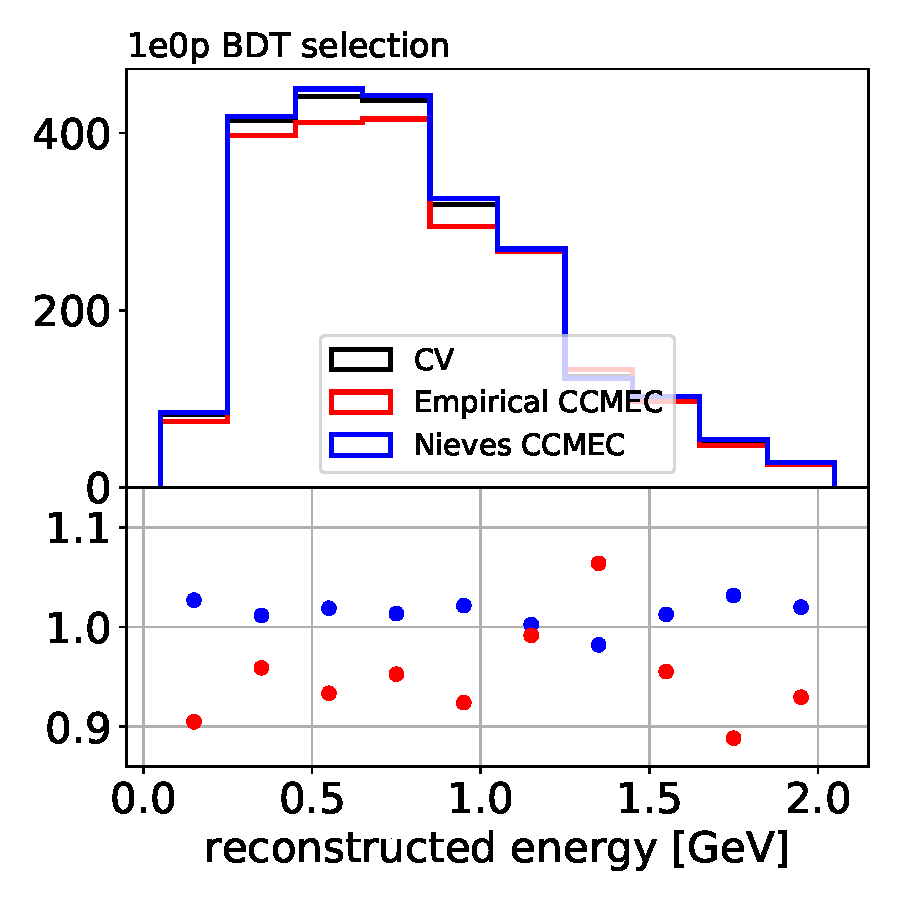
\includegraphics[width=1.00\textwidth]{Systematics/systvariations/1e0p_CCMEC.pdf}
    \end{subfigure}
    \begin{subfigure}[b]{0.3\textwidth}
    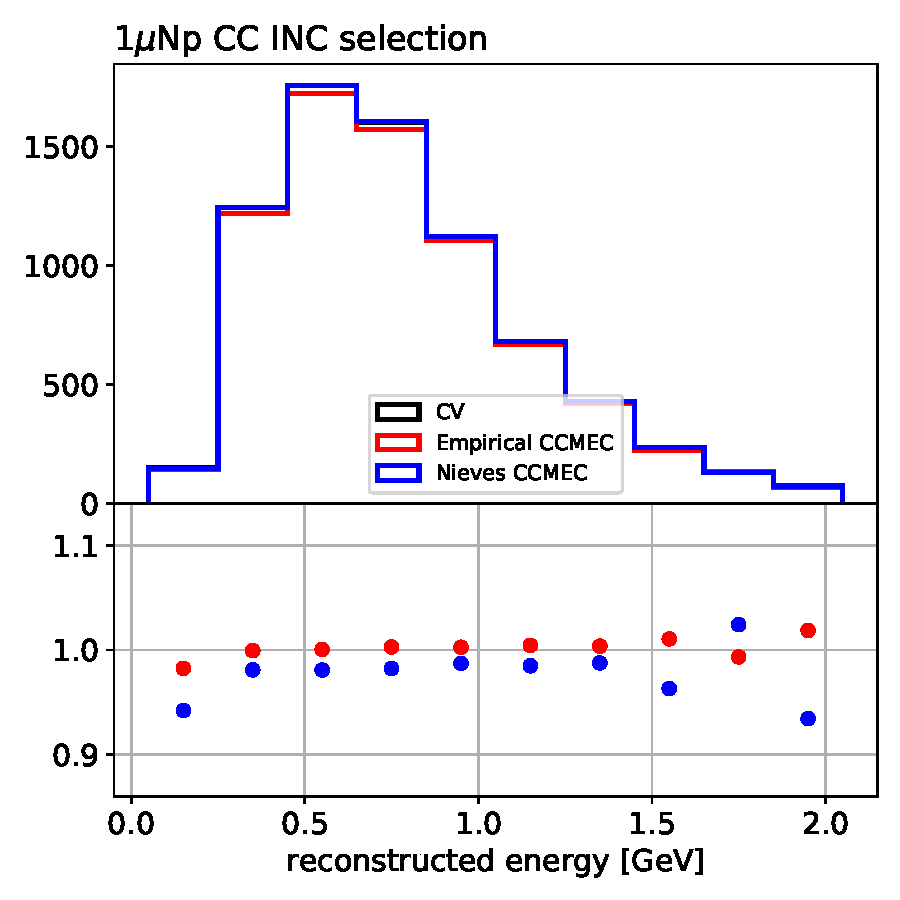
\includegraphics[width=1.00\textwidth]{Systematics/systvariations/numuCCINC_CCMEC.pdf}
    \end{subfigure}
\caption{\label{fig:ccmec} The impact of the CCMEC shape variation on selected \npsel, \zpsel, and $\nu_{\mu}$ CC INC events. }
\end{center}
\end{figure}

 %\textit{We observed a few number of large weights in the XSecShape\_CCMEC\_Genie knob which causes abnormally large excursions in the first three bins for the box cut selection as shown in Figure~\ref{fig:geniesystvars}. We didn't see the similar effect in the first bin of the \npsel BDT selection as the event with the large XSecShape\_CCMEC\_Genie weight does not pass the BDT selection. Due to these large weights, the XSecShape\_CCMEC\_Genie is currently not included in the Genie systematics calculation as well as in the sensitivity analysis because we still don't understand the source of these large weights. However, when the XSecShape\_CCMEC\_Genie knob is  included, we found that we are able to constrain it leading to similar post-constraint final sensitivities as quoted in table~\ref{tab:sensitivity}}.


\begin{comment}
\textit{A few technical complications in the treatment of the updated GENIE CV tune weights in SBNFit are still being resolved. These complications include the the need for a different procedure to account for the different treatment of event weights in systematic variations vs CV samples. Because the technical work to address these has not been fully completed and validated, the impact of cross-section and flux systematic uncertainties will be revisited between now and the February collaboration meeting.}
\textit{Note on the cross section systematics: The genie systematics is currently still under investigation. 
As mentioned above, the cross sections variations are thrown around the tuned genie central value and therefore already have the tuned central value weight folded in. 
Meanwhile, the default central value has to be multiplied with the genie central value tune weight to update it to the new cv value. 
We have to properly account for the Genie tuned central value that is already folded in into the Genie cross section weights so that the shift between the value in each universe of a variation and 
the central value in a bin is calculated correctly for systematics.}
\end{comment}
%The framework that we are using has limitations on the handling of the different weights that need to be applied to the central value and the universes. As we can only provide one weight to the framework, and we have to correct primarily for the central value, the cross section variations are currently double counting the genie tune weight, and therefore the average distributions of the universes in each genie reweighting parameters do not centered at the central value as shown in Figure~\ref{fig:geniesystvars}. This excursion from the central value resulted in the overestimation of the cross section uncertainty where the uncertainties average around 15\%, and up to 800\% in the lowest neutrino energy bin. 
%The work to fix the handling of the tuning when constructing the covariance matrix is on-going and we will update these set of plots when the fix is committed.}

\newpage

\begin{table}[H]
\centering
 \begin{tabular}{| c | c |} 
    \hline
\hline
Genie uncertainties & Description\\
\hline
%There are 49 uncertainties in this table.
MaCCQE & CCQE axial mass\\
NormCCMEC & Energy-independent normalization for CCMEC\\
MaNCEL & Axial mass for NCEL\\
EtaNCEL & Empirical parameter used to account for sea quark contribution to NCEL form factor\\
NormNCMEC & Energy-independent normalization for NCMEC\\
FracPN\_CCMEC & Varies fraction of initial nucleon pairs that are pn\\
FracDelta\_CCMEC & Varies relative contribution of $\Delta$ diagrams to total MEC cross section\\
NormCCRES & Energy-independent normalization for CCRES\\
MaCCRESshape & Shape-only CCRES axial mass\\
MvCCRESshape & Shape-only CCRES vector mass\\
NormNCRES & Energy-independent normalization for NCRES\\
MaNCRESshape & Shape-only NCRES axial mass\\
MvNCRESshape & Shape-only NCRES vector mass\\
MaCOHpi & Axial mass for COH $\pi$ production\\
R0COHpi & Nuclear radius parameter for COH $\pi$ production\\
NonRESBGvpCC1pi & Non-resonant background normalization for $\nu$p CC1$\pi$\\
NonRESBGvpCC2pi & Non-resonant background normalization for $\nu$p CC2$\pi$\\
NonRESBGvpNC1pi & Non-resonant background normalization for $\nu$p NC1$\pi$\\
NonRESBGvpNC2pi & Non-resonant background normalization for $\nu$p NC2$\pi$\\
NonRESBGvnCC1pi & Non-resonant background normalization for $\nu$n CC1$\pi$\\
NonRESBGvnCC2pi & Non-resonant background normalization for $\nu$n CC2$\pi$\\
NonRESBGvnNC1pi & Non-resonant background normalization for $\nu$n NC1$\pi$\\
NonRESBGvnNC2pi & Non-resonant background normalization for $\nu$n NC2$\pi$\\
NonRESBGvbarpCC1pi & Non-resonant background normalization for $\bar\nu$p CC1$\pi$\\
NonRESBGvbarpCC2pi & Non-resonant background normalization for $\bar\nu$p CC2$\pi$\\
NonRESBGvbarpNC1pi & Non-resonant background normalization for $\bar\nu$p NC1$\pi$\\
NonRESBGvbarpNC2pi & Non-resonant background normalization for $\bar\nu$p NC2$\pi$\\
NonRESBGvbarnCC1pi & Non-resonant background normalization for $\bar\nu$n CC1$\pi$\\
NonRESBGvbarnCC2pi & Non-resonant background normalization for $\bar\nu$n CC2$\pi$\\
NonRESBGvbarnNC1pi & Non-resonant background normalization for $\bar\nu$n NC1$\pi$\\
NonRESBGvbarnNC2pi & Non-resonant background normalization for $\bar\nu$n NC2$\pi$\\
AhtBY & A\_HT higher-twist parameter in the Bodek-Yang model scaling variable xi\_w\\
BhtBY & BHT higher-twist parameter in the Bodek-Yang model scaling variable xi\_w\\
CV1uBY & CV1u valence GRV98 PDF correction parameter in the Bodek-Yang model\\
CV2uBY & CV2u valence GRV98 PDF correction parameter in the Bodek-Yang model\\
AGKYxF1pi & Hadronization parameter, applicable to true DIS interactions only\\
AGKYpT1pi & Hadronization parameter, applicable to true DIS interactions only\\
MFP\_pi & $\pi$ mean free path\\
MFP\_N & Nucleon mean free path\\
FrCEx\_pi & Fractional cross section for $\pi$ charge exchange\\
FrInel\_pi & Fractional cross section for $\pi$ inelastic scattering\\
FrAbs\_pi & Fractional cross section for $\pi$ absorption\\
FrCEx\_N & Fractional cross section for nucleon charge exchange\\
FrInel\_N & Fractional cross section for nucleon inelastic scattering\\
FrAbs\_N & Fractional cross section for nucleon absorption\\
RDecBR1gamma & Normalization for $\Delta\to\gamma$ decays\\
RDecBR1eta & Normalization for $\Delta\to\eta$ decays\\
FrPiProd\_pi & Fractional cross section for $\pi^-$ induced $\pi$ production\\
FrPiProd\_N & Fractional cross section for nucleon-induced $\pi$ production\\
\hline
\end{tabular}
\caption{Uncertainties included in All\_Genie. The descriptions are taken from Ref.~\cite{bib:geniesupportnote}.}
\label{tab:AllGenie}
\end{table}

\begin{table}[H]
\centering
 \begin{tabular}{| c | m{8cm} | c |} 
    \hline
\hline
Genie knobs & Description & Universes \\
\hline
All\_UBGenie      & 44 GENIE knobs are varied randomly and simultaneously according to Gaussian distributions, with 1$\sigma$ uncertainties & 500\\
RPA\_CCQE\_UBGenie      & Strength of the RPA correction & 2\\
XSecShape\_CCMEC\_Genie     &  Changes the CCMEC cross section shape from the Nieves prediction (parameter value = 0) to the shape predicted by GENIE’s Empirical MEC model (parameter value = 1) & 2\\ 
AxFFCCQEshape\_UBGenie   &  Parameterization of the nucleon axial form factor & 2\\
VecFFCCQEshape\_UBGenie      &  Parametrization of the vector form factor model & 2\\  
DecayAngMEC\_UBGenie       & Changes angular distribution of nucleon cluster  & 2\\ 
ThetaDelta2NRad\_UBGenie   &  Interpolates angular distribution for $\Delta\to N+\gamma$ between isotropic (0) and $\propto \cos^2 \theta$  (1) & 2\\ 
Theta\_Delta2Npi\_Genie       &  Interpolates angular distribution for $\Delta\to N+\pi$ between Rein-Sehgal model (0) and isotropic (1) & 2\\ 
NormCCCOH\_UBGenie       &  Scaling factor for CC COH $\pi$ production & 2\\ 
NormNCCOH\_UBGenie      &  Scaling factor for NC COH $\pi$ production  & 2\\ 
\hline
\end{tabular}
\caption{List of genie systematic variations used in the Pandora eLEE analysis as described in Ref.~\cite{bib:geniesupportnote}.}
\label{tab:geniesyst}
\end{table}

\begin{figure}[H] 
    \begin{center}
    \begin{subfigure}[b]{0.48\textwidth}
    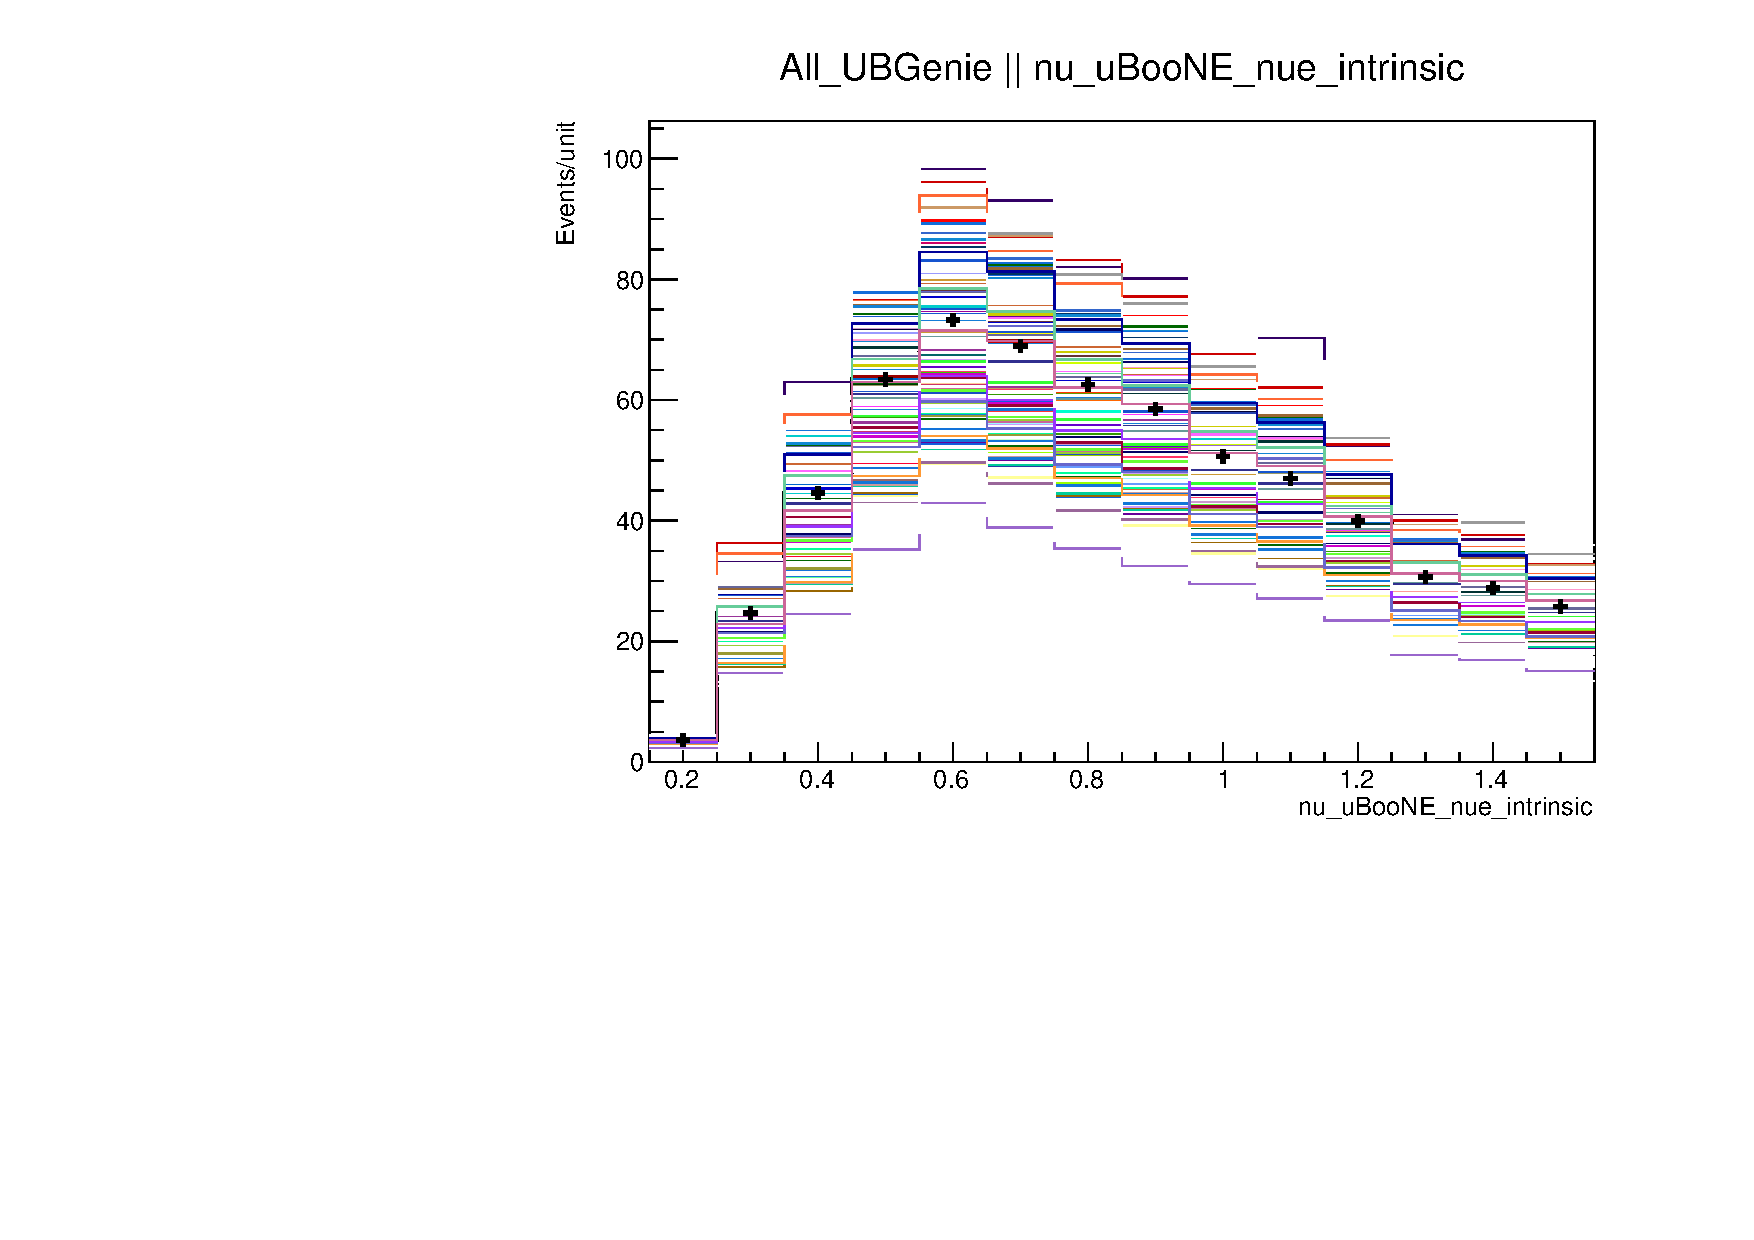
\includegraphics[width=1.00\textwidth]{Systematics/systvariations/BDT/Variation_nue_1e0p_numu_reco_e_H1_mc_collab_All_UBGenie_nu_uBooNE_nue_intrinsic_1D.pdf}
    \end{subfigure}
    \begin{subfigure}[b]{0.48\textwidth}
    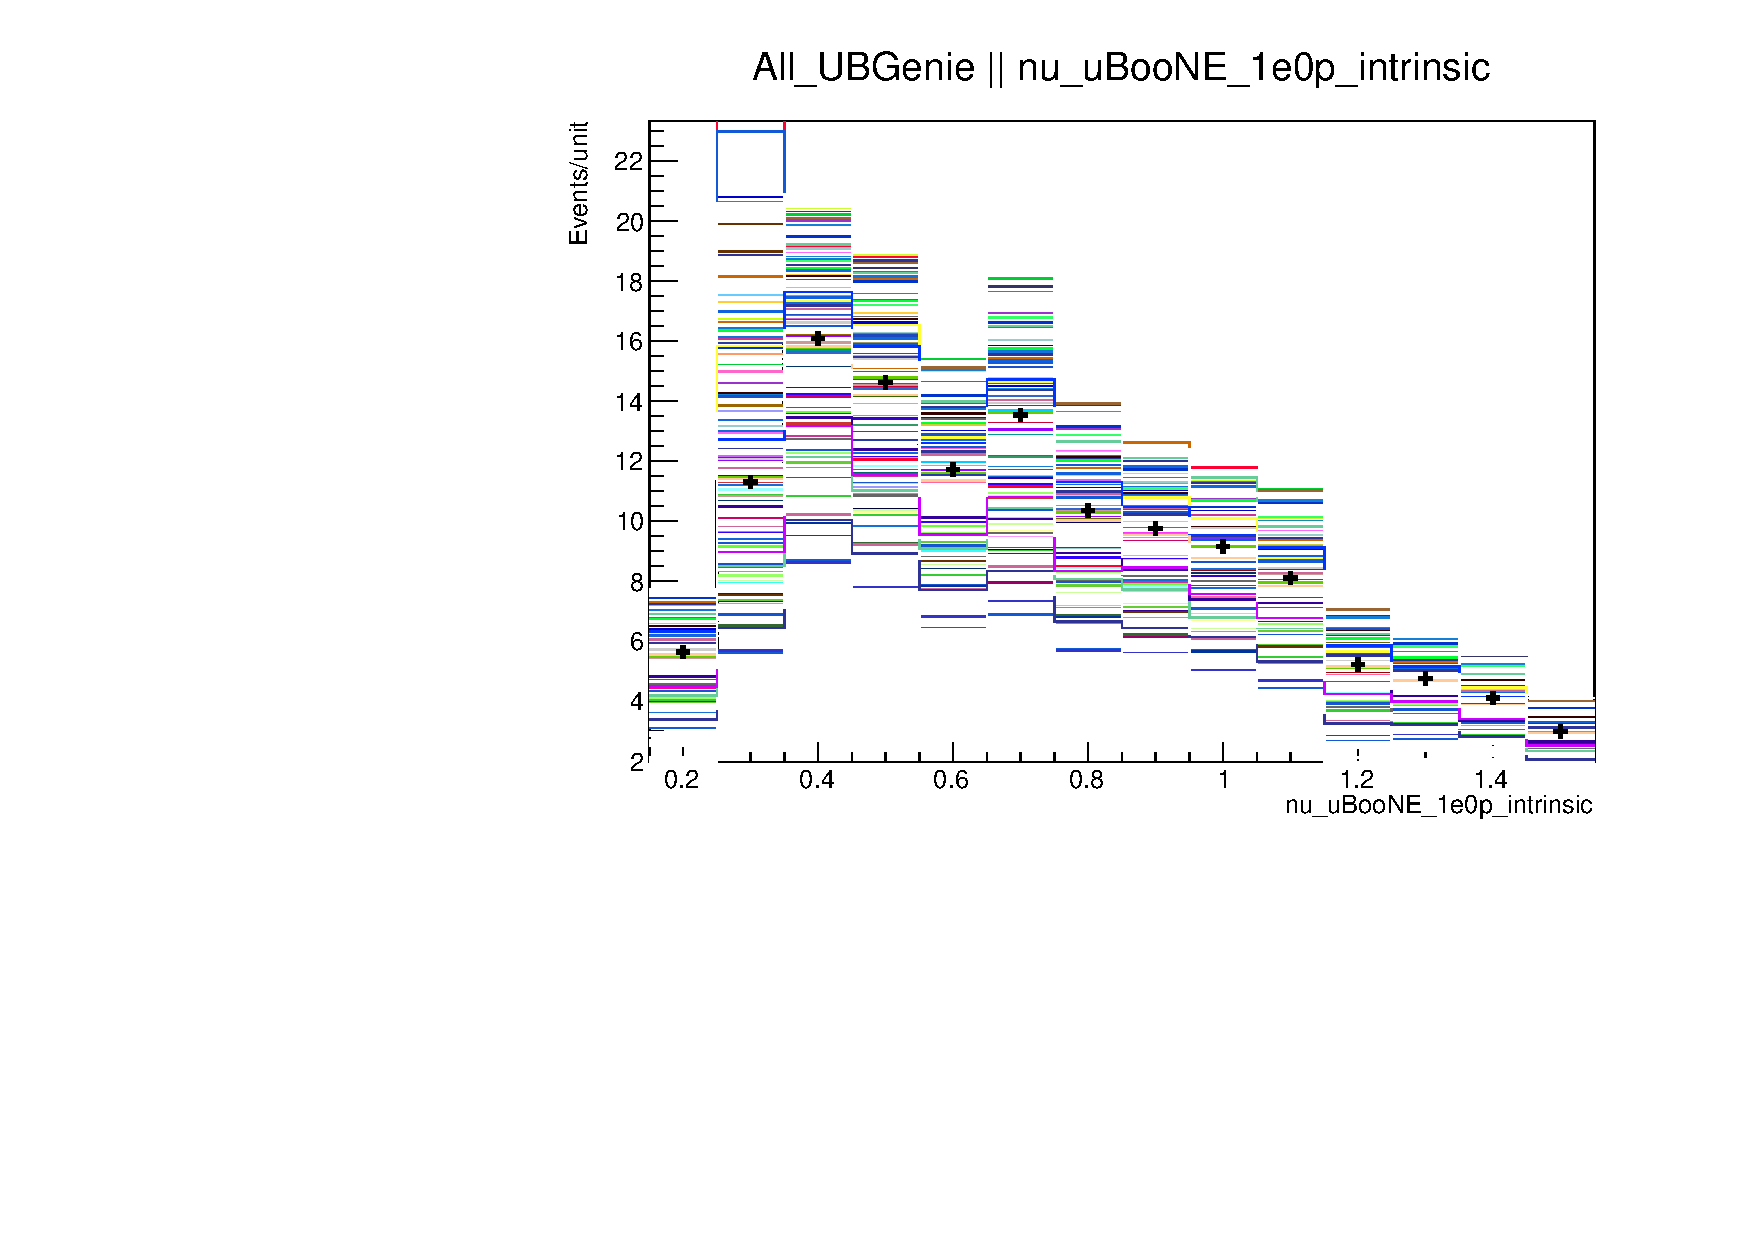
\includegraphics[width=1.00\textwidth]{Systematics/systvariations/BDT/Variation_nue_1e0p_numu_reco_e_H1_mc_collab_All_UBGenie_nu_uBooNE_1e0p_intrinsic_1D.pdf}
    \end{subfigure}
\caption{\label{fig:geniesystvars} The effects of \textit{All\_UBGenie} knobs variations on the intrinsic \nue sub-channel of the \npsel and \zpsel selection. The black crosses show the central value and each multicolored line shows a separate universe's reweighing of the central value. The magnitude of the  uncertainty in each bin corresponds to the average difference between each shifted universe and the central value in that bin.} %Note that due to the large deviation seen in the XSecShape\_CCMEC\_Genie universe with respect to the central value, we are currently excluding this knob from the systematics and sensitivity analysis.}
\end{center}
\end{figure}

\begin{figure}[ht] 
\begin{center}
    \begin{subfigure}[b]{0.48\textwidth}
    \centering
    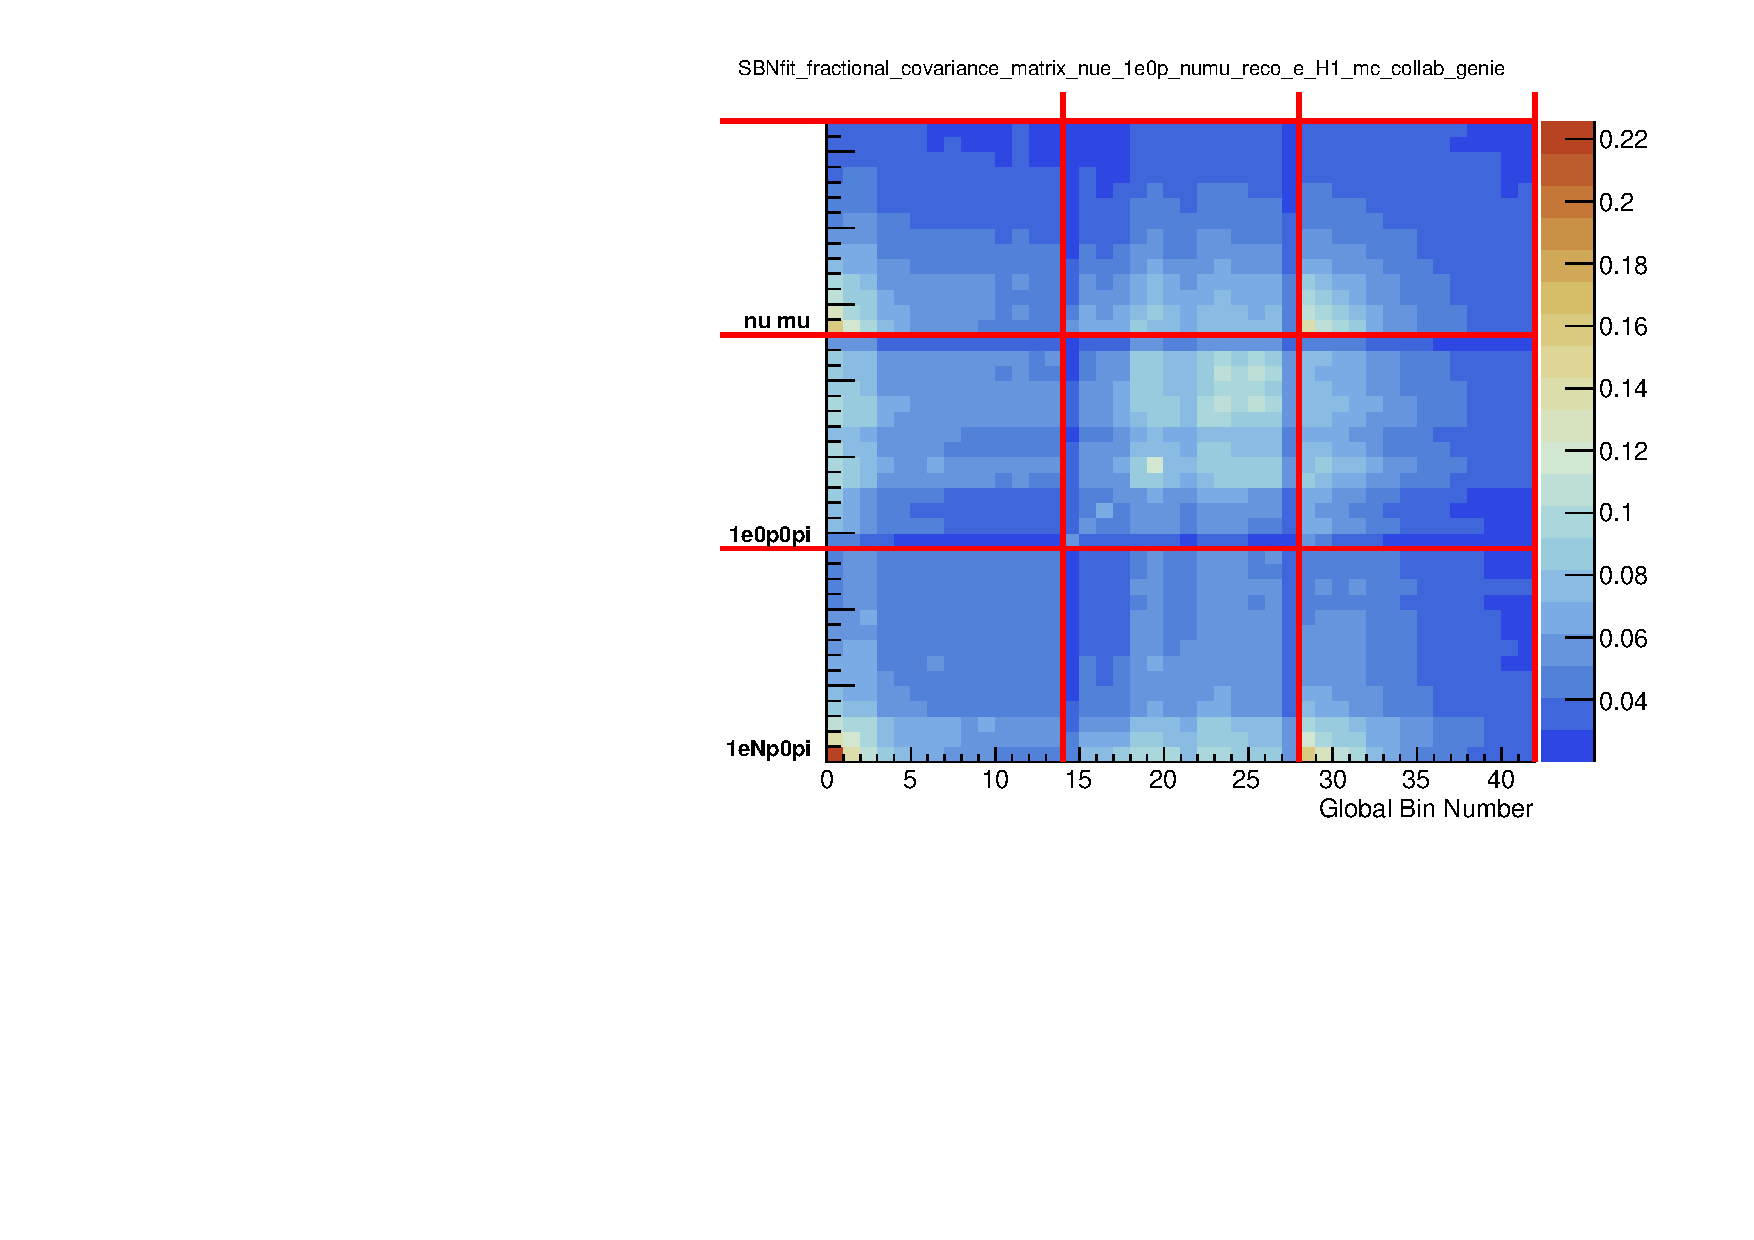
\includegraphics[width=1.00\textwidth]{Systematics/CovarianceMatrices/SBNfit_fractional_covariance_matrix_nue_1e0p_numu_reco_e_H1_mc_collab_genie_collapsed.pdf}
    \caption{genie fractional covariance matrix}
    \end{subfigure}
    \begin{subfigure}[b]{0.48\textwidth}
    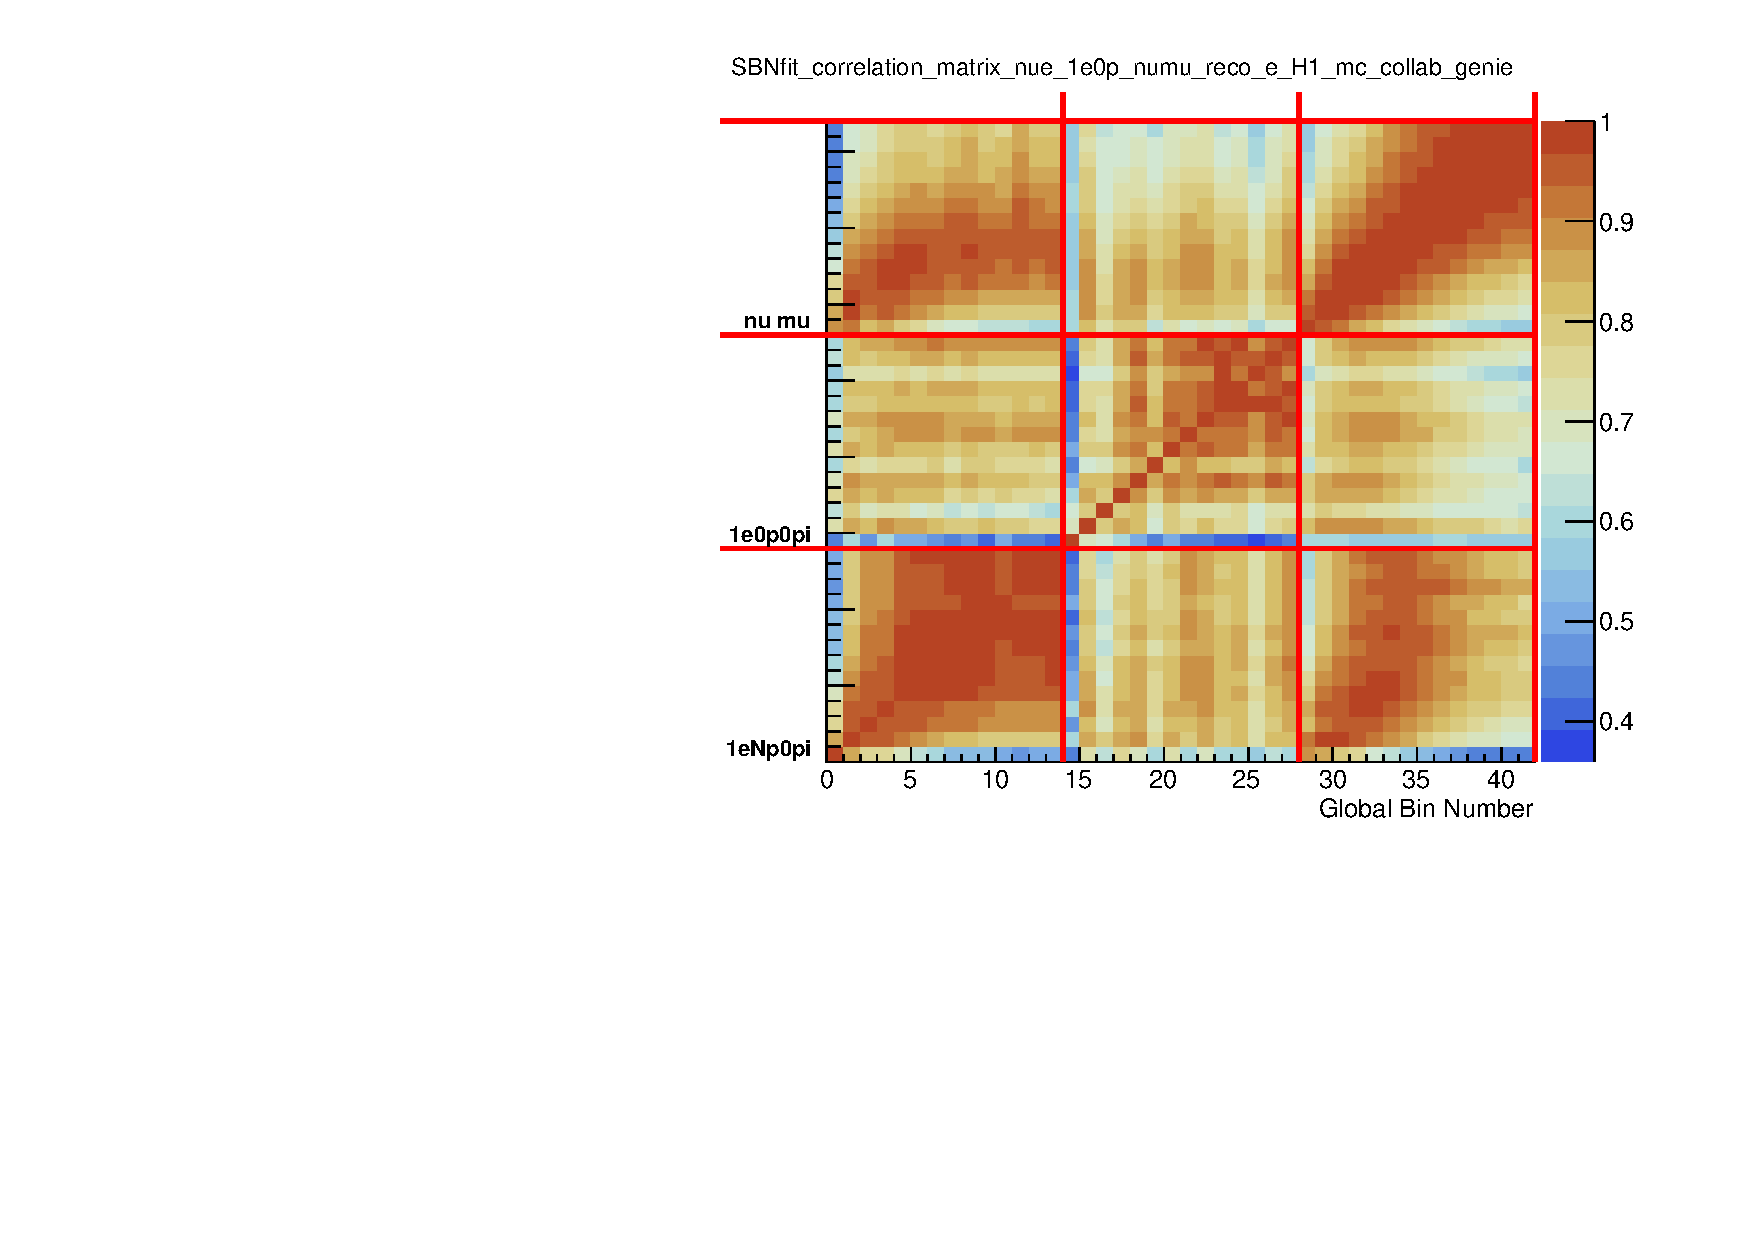
\includegraphics[width=1.00\textwidth]{Systematics/CovarianceMatrices/SBNfit_correlation_matrix_nue_1e0p_numu_reco_e_H1_mc_collab_genie_collapsed.pdf}
    \caption{genie correlation matrix}
    \end{subfigure}
\caption{\label{fig:geniematrices} Cross Section model (GENIE) only fractional covariance matrix for the 1eNp0$\pi$ selection. The global bin number starts from 0.15 GeV up to 1.55 GeV, in steps of 0.1 GeV. The \textit{XSecShape\_CCMEC\_Genie} knob is not included in these fractional matrices.}
\end{center}
\end{figure}

\subsection{Hadronic Reinteraction Uncertainties }
\label{sec:systematics:reint}
An additional type of systematic uncertainty that can be included is that related to hadrons interacting strongly with argon nuclei~\cite{bib:reintslides}. These hadronic rescatterings can induce a large momentum transfer in the hadron and thus have an impact in the reconstruction and the selection of events. Additionally, they can led to a re-classification of the event based on the final-state particles produced in the event. These uncertainties can be thought of as GEANT4 uncertainties in the cross section of a hadron's interaction with argon nuclei. The hadronic reinteraction uncertainties listed in Table~\ref{tab:g4syst} was made available for MCC9 (see DocDB 27561~\cite{bib:g4uncertainties}) and has been incorporated into the analysis. The impact on the \nue intrinsic selection is expected to be small, and the systematics have a larger impact on the background events such as the charged-current $\pi^0$ and neutral current with no $\pi$ in the final states. The effects of the larger systematics on the background events can be seen on ~\cref{fig:g4matrices}.

\begin{table}[H]
\centering
 \begin{tabular}{| c | m{6cm} | c |} 
    \hline
\hline
Reinteraction knobs & Description & Universes \\
\hline
reinteractions\_proton        &  Proton hadronic reinteractions  & ---\\ 
reinteractions\_piplus   &  $\pi^+$ hadronic reinteractions & ---\\ 
reinteractions\_piminus        & $\pi^-$ hadronic reinteractions  & ---\\
\hline
reint\_all                    &  all 3 reinteraction knobs randomly and simultaneously according to Gaussian distributions, with 1$\sigma$ uncertainties  & 1000 \\
\hline
\end{tabular}
\caption{List of hadronic reinteraction systematic variations, the reint\_all knob is used in the analysis}
\label{tab:g4syst}
\end{table}

\begin{figure}[ht] 
\begin{center}
    \begin{subfigure}[b]{0.48\textwidth}
    \centering
    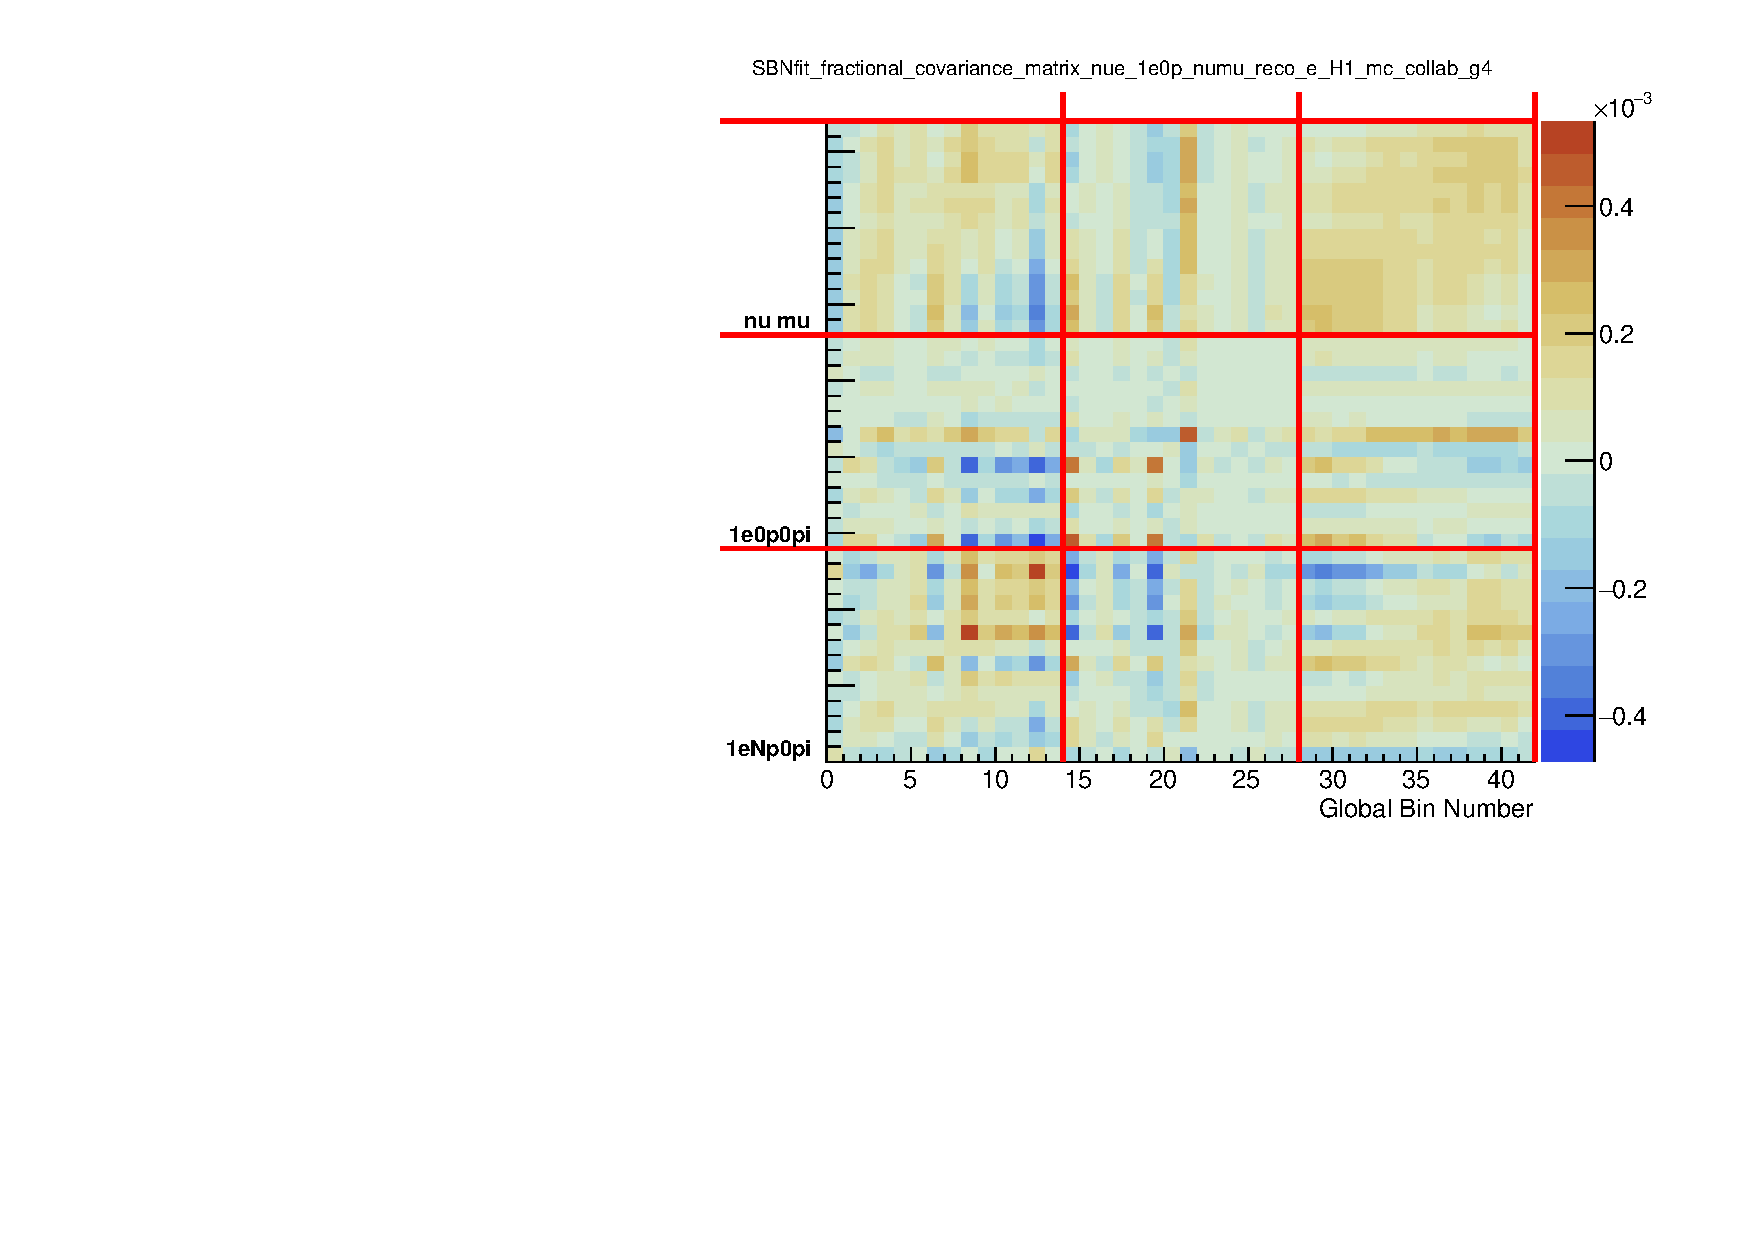
\includegraphics[width=1.00\textwidth]{Systematics/CovarianceMatrices/SBNfit_fractional_covariance_matrix_nue_1e0p_numu_reco_e_H1_mc_collab_g4_collapsed.pdf}
    \caption{g4 fractional covariance matrix}
    \end{subfigure}
    \begin{subfigure}[b]{0.48\textwidth}
    \centering
    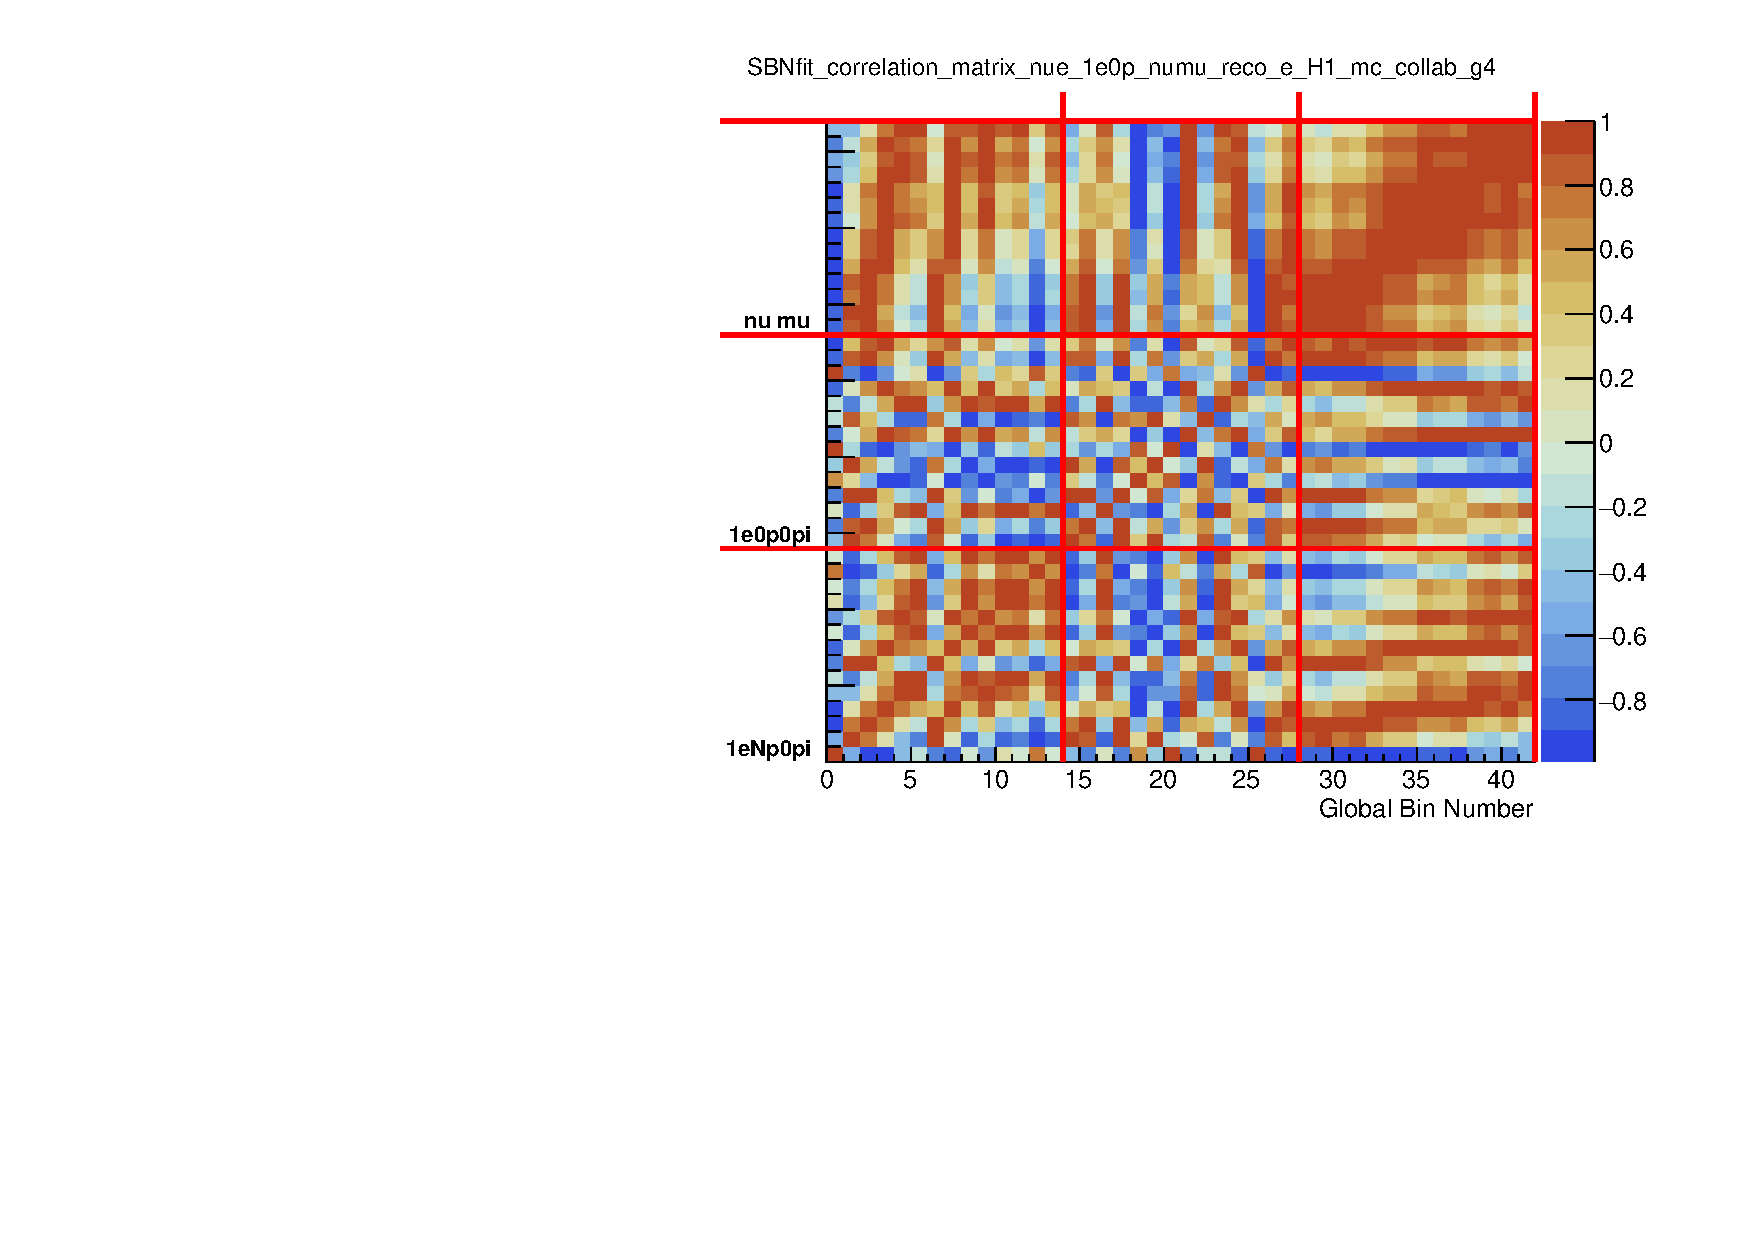
\includegraphics[width=1.00\textwidth]{Systematics/CovarianceMatrices/SBNfit_correlation_matrix_nue_1e0p_numu_reco_e_H1_mc_collab_g4_collapsed.pdf}
    \caption{g4 correlation matrix}
    \end{subfigure}
\caption{\label{fig:g4matrices} Geant4 physics models fractional covariance matrix and correlation matrix for the \npsel and \zpsel selection. The global bin number starts from 0.15 GeV up to 1.55 GeV, in steps of 0.1 GeV.}
\end{center}
\end{figure}

\subsection{Summary of the Unconstrained Systematics for the \npsel, \zpsel, and \numu selection}
\label{subsec:syst:syst_table}

This section aims to summarize the null-hypothesis (background only) cumulative fractional errors on each reconstructed energy bin of the \npsel, \zpsel, and \numu selection in Tables~\ref{tab:1eNp0pi_bdt_errors}, \ref{tab:1e0p0pi_bdtloose_errors}, \ref{tab:1e0p0pi_bdt_errors}, and \ref{tab:numu_boxcut_errors}. 
%We tend to see smaller uncertainties in the lower energy bin for the BDT selection compared to the box cut selection for the \npsel and \zpsel selection due to its higher efficiency in the low energy bins. Note that we do observe larger flux only systematics for the \npsel BDT selection in the first bin. This larger uncertainties is due to the higher efficiency in the first bin causing less events to smear down from the bin and therefore reflects a more accurate flux systematics estimation around that energy region. The flux uncertainties in this region is estimated to be ~40\% \cite{bib:fluxtechnote}.

\begin{table}[H]
\centering
\begin{tabular}{| c | c | c | c | c | c |}
\hline
Energy [GeV] & Flux Only & Genie Only  & G4 Only & Flux + Genie + G4 & Flux + Genie + G4 + Det. Syst. \\
\hline
0.15 - 0.25 & 17.33 & 47.51 & 1.09 & 50.59 & 52.38 \\
0.25 - 0.35 & 7.41 & 33.63 & 0.73 & 34.45 & 35.42 \\
0.35 - 0.45 & 6.97 & 31.51 & 1.12 & 32.29 & 33.23 \\
0.45 - 0.55 & 5.95 & 23.72 & 1.22 & 24.48 & 24.98 \\
0.55 - 0.65 & 6.06 & 22.81 & 0.62 & 23.61 & 24.28 \\
0.65 - 0.75 & 5.84 & 22.32 & 0.97 & 23.10 & 24.02 \\
0.75 - 0.85 & 5.33 & 22.60 & 1.52 & 23.27 & 24.16 \\
0.85 - 0.95 & 5.59 & 22.15 & 0.99 & 22.87 & 24.22 \\
0.95 - 1.05 & 5.40 & 21.25 & 2.23 & 22.04 & 23.84 \\
1.05 - 1.15 & 4.94 & 21.64 & 1.08 & 22.22 & 24.36 \\
1.15 - 1.25 & 5.39 & 20.74 & 1.44 & 21.48 & 32.04 \\
1.25 - 1.35 & 5.49 & 21.53 & 1.25 & 22.25 & 23.69 \\
1.35 - 1.45 & 6.17 & 20.43 & 2.31 & 21.47 & 25.33 \\
1.45 - 1.55 & 6.00 & 20.49 & 1.23 & 21.38 & 27.72 \\
\hline
\end{tabular}
\caption{Summary of the cumulative fractional errors on the flux, genie, g4, and detector systematics for the 1eNp0$\pi$ loose BDT selection}
\label{tab:1eNp0pi_bdt_errors}
\end{table}


\begin{table}[H]
\centering
\begin{tabular}{| c | c | c | c | c | c |}
\hline
Energy [GeV] & Flux Only & Genie Only  & G4 Only & Flux + Genie + G4 & Flux + Genie + G4 + Det. Syst. \\
\hline
0.15 - 0.25 & 6.82 & 24.00 & 2.17 & 25.05 & 27.66 \\
0.25 - 0.35 & 6.02 & 22.66 & 0.52 & 23.45 & 24.74 \\
0.35 - 0.45 & 6.50 & 24.86 & 0.48 & 25.70 & 26.79 \\
0.45 - 0.55 & 6.86 & 23.52 & 1.05 & 24.53 & 26.14 \\
0.55 - 0.65 & 5.70 & 29.19 & 0.36 & 29.74 & 33.27 \\
0.65 - 0.75 & 5.38 & 34.33 & 2.00 & 34.81 & 38.66 \\
0.75 - 0.85 & 7.58 & 28.37 & 0.68 & 29.37 & 33.13 \\
0.85 - 0.95 & 5.73 & 26.43 & 2.19 & 27.13 & 33.66 \\
0.95 - 1.05 & 7.51 & 30.32 & 0.43 & 31.24 & 45.36 \\
1.05 - 1.15 & 7.49 & 32.45 & 0.24 & 33.30 & 46.80 \\
1.15 - 1.25 & 5.78 & 30.74 & 0.46 & 31.29 & 35.70 \\
1.25 - 1.35 & 7.89 & 32.37 & 0.35 & 33.32 & 37.49 \\
1.35 - 1.45 & 7.34 & 29.78 & 0.54 & 30.68 & 35.17 \\
1.45 - 1.55 & 6.92 & 19.22 & 0.50 & 20.43 & 24.61 \\
\hline
\end{tabular}
\caption{Summary of the cumulative fractional errors on the flux, genie, g4, and detector systematics for the 1e0p0$\pi$ loose BDT selection}
\label{tab:1e0p0pi_bdtloose_errors}
\end{table}

\begin{table}[H]
\centering
\begin{tabular}{| c | c | c | c | c | c |}
\hline
Energy [GeV] & Flux Only & Genie Only  & G4 Only & Flux + Genie + G4 & Flux + Genie + G4 + Det. Syst. \\
\hline
0.15 - 0.25 & 9.40 & 27.01 & 1.09 & 28.62 & 29.33 \\
0.25 - 0.35 & 7.01 & 24.41 & 1.28 & 25.43 & 26.42 \\
0.35 - 0.45 & 6.27 & 22.19 & 1.14 & 23.09 & 23.65 \\
0.45 - 0.55 & 5.69 & 22.75 & 1.29 & 23.48 & 23.88 \\
0.55 - 0.65 & 5.29 & 20.63 & 1.24 & 21.34 & 22.08 \\
0.65 - 0.75 & 5.33 & 19.76 & 1.24 & 20.51 & 22.15 \\
0.75 - 0.85 & 5.70 & 19.05 & 1.13 & 19.92 & 21.26 \\
0.85 - 0.95 & 5.82 & 18.37 & 1.03 & 19.30 & 20.38 \\
0.95 - 1.05 & 6.97 & 18.23 & 1.34 & 19.56 & 22.15 \\
1.05 - 1.15 & 7.93 & 17.41 & 1.26 & 19.17 & 22.39 \\
1.15 - 1.25 & 8.99 & 17.00 & 1.45 & 19.28 & 23.48 \\
1.25 - 1.35 & 9.90 & 16.96 & 1.38 & 19.69 & 24.69 \\
1.35 - 1.45 & 11.21 & 16.47 & 1.44 & 19.98 & 26.47 \\
1.45 - 1.55 & 11.91 & 17.01 & 0.92 & 20.79 & 32.45 \\
\hline
\end{tabular}
\caption{Summary of the cumulative fractional errors on the flux, genie, g4, and detector systematics for the $\nu_\mu$ constrain selection}
\label{tab:numu_boxcut_errors}
\end{table}